\documentclass[11pt, a4paper, english, twoside, notitlepage, openright]{report}

\usepackage[a4paper, total={15cm, 22cm}]{geometry}
\usepackage{iipr}
\fancyhead[RO, LE]{ }
\fancyhead[LO]{\nouppercase \leftmark}	% Heading on odd pages: Chapter name on the left
\fancyhead[RE]{\nouppercase \rightmark} % Heading on even pages: Section on the right
\fancyfoot[LE,RO]{\thepage} % Roman numbering, foot left on even, foot right on odd pages
\fancyfoot[CE]{Double Degree in Mathematics and Computer Science} %Foot: Center, even pages
\fancyfoot[CO]{Complutense University of Madrid (UCM)} %Foot: Center, odd pages
\renewcommand{\footrulewidth}{0.4pt} % Rule on top of foot
\renewcommand{\headrulewidth}{0.4pt} % Rule below headings
\pagestyle{fancy}


\usepackage{amsmath}
\begin{document}

\pagenumbering{roman}
\begin{titlepage}

\title{\Huge{\textsc{Complexity Analysis of\\
Polynomial Algorithms}} \\
\vspace{0.5cm}
\Large{\textsc{Final Degree Project}}\\
\vspace{1.5cm}
\protect
\includegraphics[scale=0.9]{escudo_ucm.pdf}
\vspace{1.5cm}}
\author{\textbf{Ignacio Iker Prado Rujas} \\
Complutense University of Madrid (UCM) \\
Double Degree in Mathematics and Computer Science}
\date{\today}
\maketitle
\thispagestyle{empty}

\begin{center}
\textbf{Tutors:} \\
\textbf{Juan R. Delgado, Jos\'e F. Fernando \textit{\&} Jos\'e M. Gamboa} \\
\vspace{0.1cm}
Algebra Department, Mathematics Faculty
\end{center}

\end{titlepage}

\mbox{}
\thispagestyle{empty}
\newpage	
\thispagestyle{empty}
\begin{abstract} This work is about different proofs of the same fact and a computational comparison between them, looking for the most efficient one.

Let $R$ be a real closed field and $n\geq 2$. Then: 
	
(1) For every finite subset $F$ of $R^n$, the semialgebraic set $R^n\setminus F$ is a polynomial image of $R^n$. 
	
(2) Given linearly independent linear forms $h_1,\dots,h_r$ of $R^n$, the semialgebraic set $\{h_1>0,\dots,h_r>0\}\subset R^n$ is a polynomial image of $R^n$.
	
The key result here is that $\Qu:=\{x>0,y>0\}\subset R^2$ is a polynomial image of $R^2$. This assert is proved in three different ways: a first approach using some basic results in real algebraic geometry (such as Sturm's theorem and the Curve Selection Lemma) and the aid of a computer; a second and shorter one, using the composition of three rather simple polynomial maps; and a third one that applies arguments of algebraic topology, without the aid of computer computations.

(...)

\vspace{0.2cm}
\textit{Keywords.} Polynomial map, polynomial image, semialgebraic set, open quadrant, complexity.


\vspace{0.3cm}
\begin{center}
\textbf{Resumen}
\end{center}

Este trabajo contiene distintas pruebas del mismo hecho y pretende hacer una comparaci\'on computacional entre ellas, tratando de encontrar la m\'as eficiente.

Sean $R$ un cuerpo real cerrado y $n\geq 2$. Entonces: 
	
(1) Para cada subconjunto finito $F$ de $R^n$, el conjunto semialgebraico $R^n\setminus F$ es imagen polin\'omica de $R^n$. 
	
(2) Dadas formas linealmente independientes $h_1,\dots,h_r$ de $R^n$, el conjunto semialgebraico $\{h_1>0,\dots,h_r>0\}\subset R^n$ es imagen polin\'omica de $R^n$.
	
El resultado clave aqu\'i es que $\Qu:=\{x>0,y>0\}\subset R^2$ es imagen polin\'omica de $R^2$. Esta afirmaci\'on es probada de tres maneras diferentes: una primera usando algunos resultados b\'asicos de geometr\'ia algebraica real (como son el teorema de Sturm y el Lema de Selecci\'on de Curvas) y la ayuda de un ordenador; una segunda forma m\'as breve, empleando la composici\'on de tres aplicaciones polinomiales bastante sencillas; y una tercera y \'ultima en la que se utilizan  argumentos de topolog\'ia algebraica, que evitan efectuar c\'alculos en un ordenador. 

(...)

\vspace{0.2cm}
\textit{Palabras clave.} Aplicaci\'on polinomial, imagen polinomial, conjunto semialgebraico, quadrante abierto, complejidad.


\end{abstract}

\tableofcontents
\thispagestyle{empty}

\begin{chapter}{Introduction to polynomial images of $R^n$}
\pagenumbering{arabic}    % Numbering from 1

\begin{section}{Statement of the problem and main results}
\begin{definition}\label{polyMap} Given a \hyperref[realCField]{real closed field} $R$ and positive integers $m,n$ it is said that $f:=(f_1,\dots,f_n):R^m\to R^n$ is a \em polynomial map \em if $f_i\in R[{\tt x}_1,\dots,{\tt x}_m]$ for $i=1,\dots,n$. 
\end{definition}

An important example of real closed field (and the only one with the Archimedean property) if the field $\R$ of real numbers. There are several concepts, like the one of real closed field, that appear in the Introduction but that we do not recall until Appendix \ref{AA} in order to lighten the presentation and soften the reading.
	
A very famous theorem by Tarski and Seidenberg states the following:
\begin{theorem}[\em Tarski-Seidenberg\em]\label{tarskiSeidenberg} \em The image of every polynomial map $f: R^m \longrightarrow R^n$ is a \hyperref[semialgSet]{semialgebraic subset} of $R^n$. \em
\end{theorem}

In this work we study a sort of converse of this statement. In the 1990 \emph{Oberwolfach Reelle algebraische Geometrie} week, J.M. Gamboa \cite{g} proposed the following
\begin{problem}
Characterize the semialgebraic subsets of $R^n$ that are polynomial images of some $R^m$.
\end{problem}
Particularly interesting seems to be the study of those open semialgebraic subsets of $R^n$ that are polynomial images of $R^n$, because this is related with the real jacobian conjecture.
	
\begin{notation} We need to mention to which topology we refer to when we talk about closures, boundaries, etc. More specifically, the \em exterior boundary \em of a subset $S\subset R^n$ is $\delta S:=\overline{S}\setminus S$, with $\overline{S}$ being the \em closure \em of $S$ in the usual topology of $R^n$. In addition we will denote by $\overline{S}^{\text{zar}}$ the closure of $S$ with respect to the \hyperref[zariski]{Zariski topology} of $R^n$. We will say that a semialgebraic subset $A\subset R^n$ is \em Zariski-irreducible \em if its Zariski closure $\overline{A}^{\text{zar}}$ is an irreducible algebraic set.
\end{notation}
	
\begin{subsection}{Necessary conditions and examples} To begin working on this idea, we provide some necessary conditions for a set $S\subset R^n$ to be a polynomial image of $R^m$. 
	
If $m=n=1$, that is, for a polynomial function $f:R\to R$, its image $f(R)$ is either a \em singleton, \em that is, a set with a unique point if the function $f$ is constant, or an unbounded closed interval. For example if $f({\tt x})={\tt x}^2$ we have $f(R)=[0,+\infty)$, and $f(R)=R$ if $f$ is a polynomial of odd degree.
	
In the general case, by \hyperref[tarskiSeidenberg]{Tarski-Seidenberg}, $S$ must be a semialgebraic set and, as $R^n$ is semialgebraically connected, $S$ is semialgebraically connected too. In addition, by the identity principle for polynomials, $S$ is Zariski-irreducible and \hyperref[pureDim]{pure dimensional}.
	
	% Añadir el teorema de Shiota y la definición de Nash map? NO
	
But to be a polynomial image of some $R^m$ is a restrictive condition, and there are more constrains than those quoted above. 
	
\begin{definition} A polynomial map $f:R^m\to R^n$ is said to be \em semialgebraically proper at a point $p\in R^n$ \em if there exists an open neighbourhood $K$ of $p$ such that the restriction $f|_{f^{-1}(K)}:f^{-1}(K)\to K$ is a \hyperref[properMap]{semialgebraically proper map}.
\end{definition}
	
\begin{definition} A \em parametric semiline \em of $R^n$ is the image of $R$ under a non-constant polynomial map $R\to R^n$.
\end{definition}
	
It is clear that every parametric semiline is semialgebraically closed, since every polynomial map from $R$ to $R^n$ is semialgebraically proper. Let $\S_f$ denote the set of points $p\in R^n$ at which $f$ is \textbf{not} semialgebraically proper.
	
\begin{theorem}[\em Jelonek\em]\label{jelonek}\em Let $f:R^2\to R^2$ be a \hyperref[dominant]{dominant} polynomial map. Then $\S_f$ is a finite union of parametric semilines.\em
\end{theorem}
	
With these ideas in mind, we present in the following proposition some obstructions for a semialgebraic set to be a polynomial image of $R^n$. 
\begin{proposition}\label{propIntro} Let $f: R^m\to R^n$ be a polynomial map and $S:=f(R^m)$.
\begin{enumerate}[\em(1)\em]
\item $\delta S \subset\S_f$.
\begin{Proof} Suppose $p\in\delta S\setminus \S_f$. Since $p\notin\S_f$, there exists an open neighbourhood $K$ of $p$ such that the restriction $f|_{f^{-1}(K)}:f^{-1}(K)\to K$ of $f$ is proper. Thus its image $K\cap S$ is a closed subset of $K$. Hence, $p\in K\cap\overline{S}=K\cap(\overline{K\cap S})=K\cap S$, which yields in a contradiction.
\end{Proof}
\item Let $m=n=2$ and $\Gamma$ be a $1$-dimensional irreducible component of $\overline{\delta S}^{\text{zar}}$. Then $\Gamma$ is the Zariski closure of a parametric semiline of $R^2$.
\begin{Proof} As $f$ is a dominant map, $\S_f$ is, by Theorem \ref{jelonek}, a finite union of parametric semilines, say $M_1,\dots, M_s$ in $R^2$. Using (1) we get: $\Gamma\subset\overline{\delta S}^{\text{zar}}\subset \overline{\S_f}^{\text{zar}}=\bigcup_{i=1}^s\overline{M_i}^{\text{zar}}$. Lastly, using that both $\Gamma$ and the $\overline{M_i}^{\text{zar}}$'s are irreducible, $\Gamma=\overline{M_i}^{\text{zar}}$ for some index $i=1,\dots,s$.
\end{Proof}
\item Let $p:R^n\to R$ be a polynomial map which is non-constant on $S$. Then $p(S)$ is unbounded.
\begin{Proof} For each $a \in R^m$ let $\varphi_a:R\to R$ defined as $\varphi_a(t):=p(f(ta))$. Then $p(S)$ would contain the image $\varphi_a(R)$ for all $a\in R^m$. Suppose now that $\varphi_a(R)$ is bounded. Then $\varphi_a(R)$ would be a point $r_a$, and given two points $a,b\in R^m$ we would have
$$ 
\varphi_a(1)=p(f(a))=r_a=\varphi_a(0)=\varphi_b(0)=r_b=p(f(b))=\varphi_b(1).
$$ 
Then $p$ would be constant on $S$, which is a contradiction.
\end{Proof}
\end{enumerate}
\end{proposition}	
\begin{corollary} Because of statement \em (3) \em in Proposition \em \ref{propIntro}, \em all linear projections of a polynomial image $S=f(R^m)$ are either a point or unbounded. Thus, $S$ is also unbounded or a point.
\end{corollary}
	
\begin{examples}\label{introExample}
\
\begin{enumerate}[(i)]
\item The exterior of the closed unit disc $S:=\set{u^2+v^2>1}\subset R^2$ \textbf{is not} a polynomial image of $R^2$. This is so because the only irreducible component of $\overline{\delta S}^{\text{zar}}$ is the circle $\set{u^2+v^2=1}\subset R^2$ and this set is not a parametric semiline because it is bounded.
			
\item Let $S_1:=\set{uv<1}\subset R^2$ and $S_2:=\set{uv>1,u>0}\subset R^2$ (see Figure \ref{fig:introExampleii}). They both \textbf{are not} polynomial images of $R^2$ since the Zariski closure of their exterior boundaries $\overline{\delta S_1}^{\text{zar}}=\overline{\delta S_2}^{\text{zar}}$ is the hyperbola $\{uv=1\}\subset R^2$, which is not a parametric semiline.
\begin{figure}[h]\hspace{0.1cm}
\begin{subfigure}{.49\linewidth}\centering
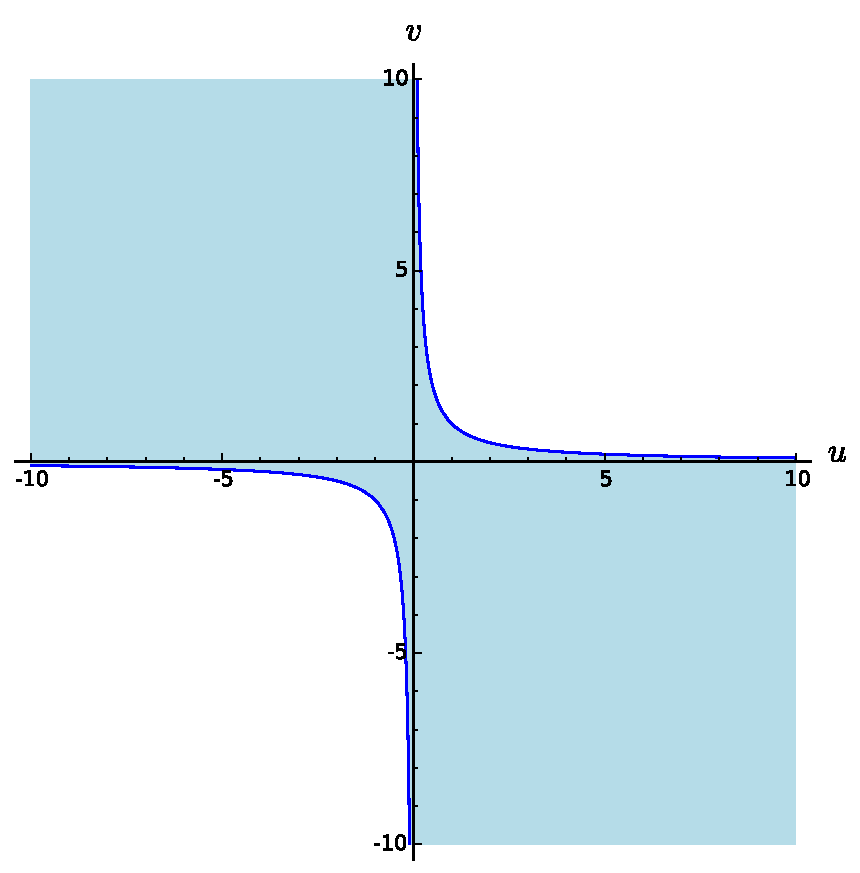
\includegraphics[width=1\textwidth]{plots/ch1_01_S_1.pdf}
\caption{$S_1:=\set{uv<1}$.\label{fig:S_1}}
\end{subfigure}
\begin{subfigure}{.49\linewidth}\centering
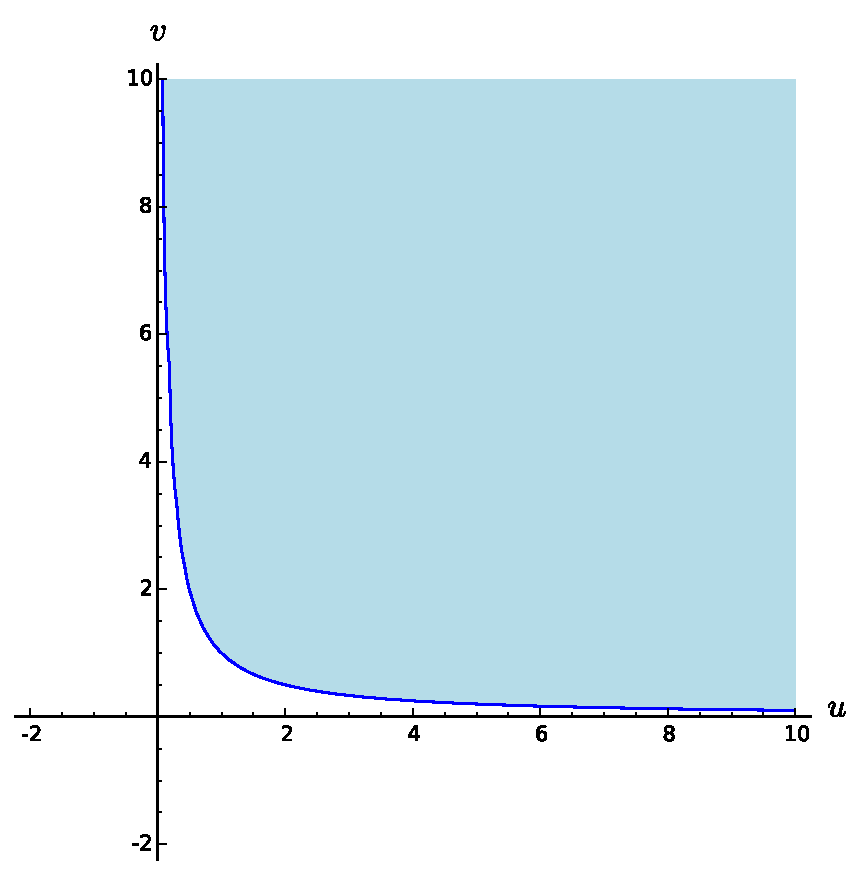
\includegraphics[width=1\textwidth]{plots/ch1_02_S_2.pdf}
\caption{$S_2:=\set{uv>1,u>0}$.\label{fig:S_2}}
\end{subfigure}\\[1ex]
\caption{Plots of the regions defined in Example \ref{introExample} (ii).\label{fig:introExampleii}}
\end{figure}
\item Let $S:=R^2\setminus\set{(0,0)}$ be the punctured plane. Then $S$ is the image of the polynomial map $(x,y) \mapsto (xy-1,(xy-1)x^2-y)$.
\item The open upper half-plane $\H:=\set{v>0}\subset R^2$ is the image of the polynomial map 
$$
R^2\to R^2,\, (x,y)\mapsto (y(xy-1),(xy-1)^2+x^2),
$$
This implies that every open half-plane is a polynomial image of $R^2$. This is probably the simplest polynomial map whose image is $\H$.
\end{enumerate}
\end{examples}
\end{subsection}
	
\begin{subsection}{Statement of the main results}
	
The main results of this chapter are generalizations of items (iii) and (iv) from Examples \ref{introExample}.
%\vspace{0.35cm}
\begin{theorem}\label{finSetTh}\em Let $n\ge2$. For every finite set $F\subset R^n$, the semialgebraic set $R^n\setminus F$ is a polynomial image of $R^n$.\em
\end{theorem}
%\vspace{0.35cm}
\begin{theorem}\label{openQuadGen}\em Let $n\ge 2$. Given independent linear forms $h_1,\dots,h_r$ of $R^n$, the open semialgebraic set $\set{h_1>0,\dots,h_r>0}$ is a polynomial image of $R^n$.\em
\end{theorem}
	
Before the paper \cite{fg} was published, the exterior boundary of all open sets that were known to be polynomial images of $R^2$ was Zariski-irreducible, and all of them were deformations of $\H$. J.M. Gamboa outlined the problem of finding if the open quadrant $\Qu:=\set{x>0,y>0}\subset R^2$ is a polynomial image of $R^2$ or not, since its exterior boundary is Zariski-reducible. The solution of this problem is a key particular case of the content of Theorem \ref{openQuadGen}. Before that, the closest known approach to look for a solution of this problem was the transformation
$$
\psi:R^2 \to R^2,\, (x,y)\mapsto(x^4y^2,x^2y^4)
$$	
whose image is $\Qu\cup\set{(0,0)}$. The answer to the first intriguing problem in this field was given in the following theorem:
\begin{theorem}\label{openQuad}\em The first open quadrant $\Qu$ is a polynomial image of $R^2$.\em
\end{theorem}
	
\begin{remark} The first proof of Theorem \ref{openQuad} consists of two parts:
\begin{itemize}
\item Choosing a ``good'' candidate to be a polynomial map whose image is close enough to $\Qu$, and giving the reasons behind this choice (see section \ref{quadReasons}). 
	
\item Checking that the image of the map is $\Qu$ indeed. After some arguments, this can be reduced to prove the non-existence of real roots of certain polynomials in one variable on certain intervals, and to compare some rational functions on those intervals. In order to do this, we use symbolic computations with tools like Sage and Maple. Because of the high degree of the involved polynomials, the actual checking of the non-existence of roots is done with a Maple package that performs \hyperref[sturm]{Sturm algorithm} and a Python programme that implements \hyperref[laguerre] {Laguerre's method}.
\end{itemize}
\end{remark}

Let us see how Theorem \ref{openQuadGen} follows from Theorem \ref{openQuad}.
		
\vspace{1mm}		
		
[Proof of Theorem \ref{openQuadGen}] After a linear change of coordinates we can suppose that $h_1:={\tt x}_1,\dots,h_r:={\tt x}_r$, so we only have to prove that for every pair of positive integers $r\leq n$ the semialgebraic set $\{x_1>0,\dots,x_r>0\}\subset R^n$ is a polynomial image of $R^n$. This is reduced to prove the following two steps:
\begin{itemize}
\item $\H:=\{x_1>0\}\subset R^2$ and $\Qu:=\{x_1>0,\,x_2>0\}\subset R^2$ are polynomial images of $R^2$, which is true, respectively, by Example \ref{introExample} (iv) and Theorem \ref{openQuad}.
\item This implies that $\mathscr{O}:=\{x_1>0,\, x_2>0,\, x_3>0\}\subset R^3$ is a polynomial image of $R^3$. Indeed, let $f,g:R^2 \rightarrow R^2$ be polynomial maps whose respective images are $\H$ and $\Qu$. Let us define:
\begin{align*}
(f,\text{id}_R): R^3=R^2\times R&\longrightarrow R^3= R^2\times R\\
(x_1,x_2,x_3) &\longmapsto (f_1(x_1, x_2),\, f_2(x_1, x_2),\, x_3)\\
(\text{id}_R,g): R^3=R\times R^2&\longrightarrow R^3= R\times R^2\\
(x_1,x_2,x_3) &\longmapsto (x_1,\, g_1(x_2, x_3),\, g_2(x_2, x_3)).
\end{align*}
Then, $\mathscr{O}$ is the image of the polynomial map 
\begin{align*}
H:=(\text{id}_R,g)\circ(f,\text{id}_R):R^3&\longrightarrow R^3\\
(x_1,x_2,x_3) &\longmapsto (f_1(x_1, x_2),\, g_1(f_2(x_1, x_2), x_3),\, g_2(f_2(x_1, x_2), x_3)).
\end{align*}
\end{itemize} 
Once the case $n=3$ is solved the case of arbitrary $n$ follows straightforwardly, by taking $g \times \overset{k}{\cdots} \times g: R^n \longrightarrow R^n$ when $n=2k$ and $H \times g \times \overset{k-1}{\cdots} \times g: R^n \longrightarrow R^n$ when $n=2k-1$. \qed

\vspace{1mm}
		
The original proofs of Theorems \ref{finSetTh} and \ref{openQuad} are written for $R:=\R$. As for both theorems explicit polynomial maps are given, the results can be extended to arbitrary real closed field $R$ by the \hyperref[TP]{Transfer Principle}.
\end{subsection}
\end{section}

\begin{section}{Complementary set of a finite set}
	
We proceed to prove Theorem \ref{finSetTh}:
	
\vspace{1mm}
	
[Proof of Theorem \ref{finSetTh}] Let $F:=\{p_1,\dots,p_k\}$. Let us see that it suffices to prove the result for points of the form $p_j:=(a_j,\vec{0})\in\R\times\R^{n-1}$. After a linear change of coordinates we can assume that the first coordinates of the given points are pairwise distinct. 

In other words, we denote $p_j:=(a_{1j},\dots,a_{nj})$ and we may suppose that $a_{1j}\neq a_{1\ell}$ when $j\neq\ell$. Then, there exists a polynomial $P_1\in\R[{\tt t}]$ such that $P_1(a_{1j})=a_{nj}$, with $j = 1,\dots, n$, and denoting $x':=(x_1,\dots,x_{n-1})$, we  define the polynomial map 
$$
h_1:\R^n\to\R^n,\, (x',x_n)\mapsto (x',x_n+P_1(x_1)).
$$
Indeed $h_1$ is bijective. Note first that every point of $\R^n$ has a preimage in $\R^n$, namely if $x:=(x_1, \dots,x_n)$, then $z:=(x',x_n-P_1(x_1))$ satisfies $h_1(z)=x$ and $h_1$ is onto. As for being injective, let $x,y\in\R^n$ such that 
$$
h_1(x)=(x_1,\dots,x_n+ P_1(x_1))=(y_1,\dots,y_n+ P_1(y_1))=h_1(y).
$$ 
Then $x_i=y_i$ for $i=1,\dots,n-1$. Also $x_n+P_1(x_1)=y_n+P_1(y_1)$ and $P_1(x_1)=P_1(y_1)$ because $x_1= y_1$. Therefore $x_n=y_n$ and $x=y$.
		
Now, for $p_j':=(a_{1j},\dots,a_{(n-1)j},0)$ we have $h_1(p_j')=p_j$. Analogously, there exists $P_2\in\R[{\tt t}]$ such that $P_2(a_{1j}) = a_{(n-1)j}$, and define the polynomial bijection
$$
h_2:\R^n\longrightarrow \R^n,\,(x'',x_{n-1},x_n)\mapsto (x'',x_{n-1}+P_2(x_1),x_n),
$$
where $x'':=(x_1,\dots,x_{n-2})$. Then $h_2(p_j'')=p_j'$ for $p_j''= (a_{1j},\dots,a_{(n-2)j},0,0)$. In this way the polynomial bijection $h_1\circ h_2:\R^n\to\R^n$ satisfies
$$
(h_1\circ h_2)(p_j'')=h_1(h_2(p_j''))=h_1(p_j')=p_j,
$$
and we can inductively construct a polynomial bijection $h:\R^n\rightarrow\R^n$ such that $h(q_j)=p_j$ for $q_j:=(a_{1j},\vec{0})\in\R\times\R^{n-1}$. Now let $G:=\{q_1,\dots,q_k\}$ and suppose that there exists a polynomial map $g:\R^n\rightarrow\R^n$ such that $g(\R^n)=\R^n\setminus G$. Then $(h\circ g)(\R^n) = \R^n \setminus F$, which concludes the first part of the proof. Thus in what follows we suppose that $p_j:=(a_j,\vec{0})$.
		
We claim that the image of the polynomial map $f:=(f_1,\dots,f_n)$ defined as:
$$
f({\tt x}):=\left({\tt x}_1{\tt x}_2-r+a_1,\ {\tt x}_1^{4}\rho({\tt x})+{\tt x}_1^{2}\sigma({\tt x})+{\tt x}_2,\ {\tt x}_3,\dots,\ {\tt x}_n\right)\quad\text{for ${\tt x}:=({\tt x}_1,\ldots,{\tt x}_n)\in\R^n$}
$$
is $\R^n\setminus F$, where $r$ is an integer such that $r\neq a_1-a_j$ for $j=1,\dots,k$,  
$$
\sigma({\tt x}):=\sum_{j=3}^n{\tt x}_j^2 \, \, \text{ and } \, \, \rho({\tt x}):=\prod_{j=1}^k({\tt x}_1{\tt x}_2-r+a_1-a_j).
$$
First, suppose that there exists $b:=(b_{1},\dots,b_{n})\in R^n$ with $f(b)=p_\ell$ for some $\ell=1,\dots,k$. Then $f_1(b)=b_1b_2-r+a_1=a_\ell$. Thus the $\ell^{th}$-factor of the polynomial $\rho$ evaluated at $x:=b$ is
$$
b_1b_2-r+a_1-a_\ell=a_\ell-a_\ell=0,
$$		 
and $\rho(b)=0$. In addition, the equality $f(b)=p_\ell=(a_{_\ell},\vec{0})$ implies that $f_i(b)=0$ for $i=2,\dots,n$. In particular, as $f_i\equiv\text{id}$ for $i=3,\dots,n$ we get $b_i=0$ for $i=3,\dots,n$. Consequently $\sigma(b)=0$. Since $\sigma(b)=\rho(b)=0$ we get $b_2=f_2(b)= 0$, so $b_2=0$ and $a_{\ell}=f_1(b)=a_1-r$, that is, $r=a_1-a_\ell$, which is a contradiction. So $\text{im}(f)\subset \R^n\setminus F$.
Conversely, let $u:=(u_1,\dots,u_n)\in\R^n\setminus F$. We must prove that the system of polynomial equations:
\[ \begin{cases} 
f_1({\tt x})={\tt x}_1{\tt x}_2-r+a_1=u_1 \\
f_2({\tt x})={\tt x}_1^4\rho({\tt x})+{\tt x}_1^2\sigma({\tt x})+{\tt x}_2=u_2 \\
f_j({\tt x})={\tt x}_j=u_j,\quad j\geq 3
\end{cases}  \]
has a solution.
\begin{enumerate}[(i)]
\item If $u_1=a_1-r$ then $f(0,u_2,\dots,u_n)=u$.
\item If $u_1\neq a_1-r$ we use the first equation to substitute 
\end{enumerate}
$$
{\tt x}_2=\frac{u_1-a_1+r}{{\tt x}_1} \quad \text{ and } \quad {\tt x}_j=u_j \quad \text{ for } j\geq 3.
$$ 
Next, we expand $f_2({\tt x})$:
$$
{\tt x}_1^4\rho({\tt x})+x_1^2\sigma({\tt x})-u_2=-{\tt x}_2=-\frac{u_1-a_1+r}{{\tt x}_1},
$$ 
and multiplying by ${\tt x}_1$ we get 
\begin{equation}\label{quintica}
{\tt x}_1^5\rho({\tt x})+{\tt x}_1^3\sigma({\tt x})-u_2{\tt x}_1+(u_1-a_1+r)=0.
\end{equation}
Then, $\rho({\tt x})=\prod_{j=1}^k(u_1-a_j) \text{ and } \sigma({\tt x})=\sigma(u)$. Now it is clear that each solution $x_1$ of equation \eqref{quintica} must be a nonzero root of the polynomial:
$$
Q({\tt t})=\Big(\prod_{j=1}^k(u_1-a_j)\Big){\tt t}^{5}+\sigma(u){\tt t}^{3}-u_2{\tt t}+(r-a_1+u_1),
$$
which has odd degree, and so it has a real root, unless 
$$
\prod_{j=1}^k(u_1-a_j)=\sigma(u)=u_2=0.
$$ 
If this were the case, then $u_1=a_j$ for some $j= 1,\dots,k$ and $u_2=u_3=\cdots=u_k=0$. This is not possible because $u\not\in F$. Thus, $Q({\tt t})$ has a real root, say $b_1$, and in fact $b_1\neq0$ because $Q(0)=r-a_1+u_1\neq 0$.
Finally, 
$$
f\left(b_1,\ \frac{u_1-a_1+r}{b_1},\ u_3,\ \dots,\ u_n\right)=u,
$$
as required.

\qed
\end{section}
\end{chapter}

\begin{chapter}{The open quadrant $\Qu$ problem: First proof}
\begin{section}{How to find a ``potential'' map to solve the problem}\label{quadReasons}
		
It is worthwhile mentioning that though the open interval $I:=(0,+\infty)$ is the image of $\R^2$ under the polynomial map $h:\R^2\to\R,\, (x,y)\mapsto (xy-1)^2+x^2$, see Figure \ref{fig:h(x,y)}, the interval $I$ is not a polynomial image of $\R$ because polynomial images of the real line are closed subsets of $\R$.
\begin{figure}[h]
\begin{center}
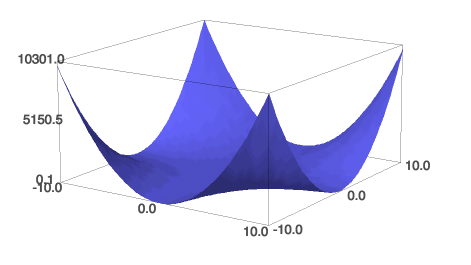
\includegraphics[width=0.8\textwidth]{plots/ch1_03_f(x,y).png}
\caption{$h({\tt x},{\tt y})=({\tt x}{\tt y}-1)^2+{\tt x}^2$.\label{fig:h(x,y)}}
\end{center}
\end{figure}
		
However, although $h(\R^2)=I$, the polynomial $h$ does not help to obtain $\Qu$ at all:
\begin{remark}
There is no polynomial map $f:=(P_1, P_2):\R^2\to\R^2$ satisfying $f(\R^2)=\Qu$ and $P_1({\tt x},{\tt y})=({\tt x}{\tt y}-1)^2+{\tt x}^2$.
\end{remark}
The proof of this remark relies on a suitable use of the Curve Selection Lemma (\cite[VIII.2.6]{abr}) to approach a point $(\lambda^2,0)\in\overline{\Qu}$ with $\lambda>0$, to get a contradiction.
		
\vspace{1mm}

On the topic of finding a polynomial map $\Phi:\R^2\to\R^2$ that satisfies $\Phi(\R^2)=\Qu$, ``a major difficulty" is the following:
\begin{center}
\begin{tabular}{rr}
$\qquad \qquad\quad$ \fbox{\textit{The closure of its image must contain the positive half-axes.}} & $\quad \quad$ ($\clubsuit$)
\end{tabular}
\end{center}
\begin{remark} Using Theorem \ref{finSetTh}, we just need to find a polynomial map $$\P=(\F,\G):\R^2\to\R^2$$ such that $\P(\R^2)$ is the disjoint union of $\Qu$ and a set with finite preimage, say $\P(\R^2)=\Qu\ \sqcup F$ with $\P^{-1}(F)$ a finite set. Suppose for a while this is proved. Then, by Theorem \ref{finSetTh}, there exists a polynomial map $\varphi:\R^2\to\R^2$ such that $\varphi(\R^2)=\R^2\setminus\P^{-1}(F)$ and the polynomial map $\Phi:=\P\circ\varphi$ satisfies
$$
\Phi(\R^2)=\P(\varphi(\R^2))=\P(\R^2\setminus\P^{-1}(F))=\P(\R^2)\setminus F=(\Qu\ \sqcup F)\setminus F=\Qu.
$$ 
\end{remark}
We are going to define a map $\P:=(\F,\G)$ that accomplish this task, with the set $F$ being $F:=\set{(-1,0),(0,-1)}$. If we were able to find such map $\P$, then condition ($\clubsuit$) will immediately be satisfied. 
		
\vspace{1mm}

Suppose for a while that such a map $\P$ exists. Then, for every $\lambda,\mu\ge 0$ there will exist \hyperref[curveGerms]{Nash half-branch curve germs} $\alpha_{\lambda}(s),\beta_{\mu}(s)$ which cannot be extended to $0$ and such that:
$$
\lim_{s\rightarrow 0} P(\alpha_{\lambda}(s))=(\lambda^2,0)\qquad \text{and} \qquad \lim_{s\rightarrow 0} P(\beta_{\mu}(s))=(0,\mu^2).
$$
We can try parameterizations of the form:
$$
\alpha_{\lambda}(s):=\left(s^{n_{\lambda}},\frac{a_{\lambda 0}+a_{\lambda 1}s+\cdots}{s^{m_{\lambda}}}\right)
\quad \text{ and } \quad
\beta_{\mu}(s):=\left(\frac{b_{\mu 0}+b_{\mu 1}s+\cdots}{s^{\ell_{\mu}}},s^{k_{\mu}}\right).
$$
Then $a_{\lambda 0},b_{\mu 0}$ must be constants (except maybe for finitely many values of $\lambda$ and $\mu$). This leads us to choose curves of the type:
$$
\alpha_{\lambda}(s):=\left(s^{n_{\lambda}},\frac{1+a_{\lambda 1}s+\cdots}{s^{m_{\lambda}}}\right)
\quad \text{ and } \quad
\beta_{\mu}(s):=\left(\frac{1+b_{\mu 1}s+\cdots}{s^{\ell_{\mu}}},s^{k_{\mu}}\right),
$$
and among them we make the simplest choice: 
$$
\alpha_{\lambda}(s):=\left(s,\frac{1+a_{\lambda }s}{s}\right)
\quad \text{ and } \quad
\beta_{\mu}(s):=\left(\frac{1+b_{\mu }s}{s},s^{3}\right).
$$
The following pair of polynomials:
\begin{equation*}
\boxed{
\begin{aligned}
\F({\tt x},{\tt y})&:=(1-{\tt x}^3{\tt y}+{\tt y}-{\tt x}{\tt y}^2)^2+({\tt x}^2{\tt y})^2&=&\ \F_1^2+\F_2^2 \\
\G({\tt x},{\tt y})&:=(1-{\tt x}{\tt y}+{\tt x}-{\tt x}^4{\tt y})^2+({\tt x}^2{\tt y})^2&=&\ \G_1^2+\G_2^2\\
\end{aligned}
}
\end{equation*}
enjoy a nice behavior along these curves, as figure \ref{fig:plotFG} show.
\begin{figure}[h]\hspace{-0.15cm}
\begin{subfigure}{.49\linewidth}\centering
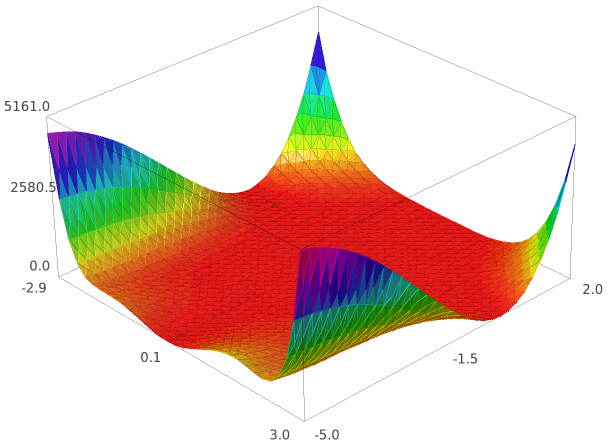
\includegraphics[width=1\textwidth]{plots/ch1_04_F.png}
\caption{$\F({\tt x},{\tt y}):=(1-{\tt x}^3{\tt y}+{\tt y}-{\tt x}{\tt y}^2)^2+({\tt x}^2{\tt y})^2$.\label{fig:F}}
\end{subfigure}
\begin{subfigure}{.50\linewidth}\centering
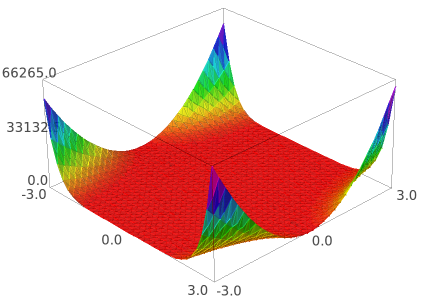
\includegraphics[width=1\textwidth]{plots/ch1_05_G.png}
\caption{$\G({\tt x},{\tt y})=(1-{\tt x}{\tt y}+{\tt x}-{\tt x}^4{\tt y})^2+({\tt x}^2{\tt y})^2$.\label{fig:G}}
\end{subfigure}\\[1ex]
\caption{Plots of the polynomials $\F,\G:\R^2\longrightarrow\R$.\label{fig:plotFG}}
\end{figure}
Next, notice that
\begin{enumerate}[(a)]
\item $\cdot$ $\F_1\circ\alpha_\lambda=1-a_{\lambda}-a_{\lambda}^{2} s-s^{2}-a_{\lambda} s^{3}\in\R[s,a_{\lambda}]$,
$\qquad\qquad\qquad \,\, \, \,   \F_1\circ\alpha_{\lambda }(0)=1-a_{\lambda. }$ \newline
$\cdot$ $\F_1\circ\beta_{\mu}=-3\,b_{\mu}s-3 \,b_{\mu}^{2} s^{2}-{\left(b_{\mu}^{3}-1\right)}s^{3}-s^{5}-b_{\mu}s^{6}\in\R[s,b_{\mu}]$,
$\, \F_1\circ\beta_{\mu}(0)=0$.
				
\item $\cdot$ $ \G_1\circ\alpha_{\lambda } = {\left(1-a_{\lambda} \right)}s-s^{3}-a_{\lambda} s^{4} \in\R[s,a_{\lambda}]$,
$\qquad\qquad\qquad\qquad\, \, \, \, \,\G_1\circ\alpha_{\lambda }(0)=0$.

$\cdot$ $\G_1\circ\beta_{\mu}=1-3\, b_{\mu}-6\,b_{\mu}^{2}s-{\left(4\,b_{\mu}^{3}+1\right)}s^{2}-{\left(b_{\mu}^{4}+ b_{\mu}\right)}s^{3}\in\R[s,b_{\mu}], \, \, \G_1\circ\beta_{\mu}(0)=1-3b_{\mu}$.
		
\item $\cdot$ $\F_2\circ\alpha_{\lambda }= s+a_{\lambda} s^{2} = \G_2\circ\alpha_{\lambda}\in\R[s,a_{\lambda }]$.
			
$\cdot$ $\F_2\circ\beta_{\mu}= s+2 \, b_{\mu} s^{2}+b_{\mu}^{2} s^{3} = \G_2\circ\beta_{\mu}\in\R[s,b_{\mu}]$.
				
$\cdot$ $\F_2\circ\alpha_{\lambda }(0)=\G_2\circ\alpha_{\lambda}(0)=\F_2\circ\beta_{\mu}(0)=\G_2\circ\beta_{\mu}(0)=0$.
\end{enumerate}
All of these map compositions were computed by Sage. Thus, we get the following properties:
		
\begin{enumerate}[(i)]
		
\item The polynomials $\F,\G$ are non-negative in $\R^2$.
		
\item $\cdot$ $\F^{-1}(0)=\F_1^{-1}(0)\cap \F_2^{-1}(0)=\{(0,-1)\}\xmapsto{\ \P\ }\set{(0,1)}$.
			
$\cdot$ $\G^{-1}(0)=\G_1^{-1}(0)\cap \G_2^{-1}(0)\ =\, \{(-1,0)\} \xmapsto{\ \P\ } \set{(1,0)}$.
		
\item $\cdot$ $\P\circ\alpha_{\lambda}=(\F\circ\alpha_{\lambda },\G\circ\alpha_{\lambda})=$
			
$\arraycolsep=2pt\def\arraystretch{1.2}
\begin{array}{l}
\left(\right.a_{\lambda}^{2}-2 \,a_{\lambda}+1+2 \,{(a_{\lambda}^{3}-a_{\lambda}^{2})}s+{(a_{\lambda}^{4}+2 \, a_{\lambda}-1)} s^{2}+ \,a_{\lambda}^{2} s^{3}+\\
\quad {(2\, a_{\lambda}^{3}+a_{\lambda}^{2}+1)}s^{4}+2 \,a_{\lambda} s^{5}+a_{\lambda}^{2} s^{6},\\		
\ {(a_{\lambda}^{2}-2 \ a_{\lambda}+2)} s^{2}+2 \, a_{\lambda} s^{3}+{(a_{\lambda}^{2}+2 \,a_{\lambda}-2)}s^{4}+\\
\quad \,2 \,{(a_{\lambda}^{2}-a_{\lambda})}s^{5}+s^{6}+2\,a_{\lambda} s^{7}+a_{\lambda}^{2}s^{8}\left.\right).
\end{array}
$
				
$\cdot$ $\P\circ\beta_{\mu}=(\F\circ\beta_{\mu},\G\circ\beta_{\mu})=
$
				
				$\arraycolsep=2pt\def\arraystretch{1.2}
\begin{array}{l}
\left(\right.{(9 \,b_{\mu}^{2}+1)}s^{2}+2 \,{(9 \,b_{\mu}^{3}+2\,b_{\mu})}s^{3}+3\,{(5\,b_{\mu}^{4}+2\,b_{\mu}^{2}-2\,b_{\mu})}s^{4}+\\
\quad 2\,{(3 \,b_{\mu}^{5}+2\,b_{\mu}^{3}-3\,b_{\mu}^{2})}s^{5}+{(b_{\mu}^{6}+b_{\mu}^{4}-2\,b_{\mu}^{3}+6\,b_{\mu}+1)} s^{6}+\\
\quad 12\,b_{\mu}^{2} s^{7}+2\,{(4\,b_{\mu}^{3}-1)}s^{8}+2\,{(b_{\mu}^{4}-b_{\mu})}s^{9}+s^{10}+2\,b_{\mu}s^{11}+b_{\mu}^{2} s^{12},\\
					\ 9 \, b_{\mu}^{2}-6 \, b_{\mu}+1+12 \, {(3 \, b_{\mu}^{3} - b_{\mu}^{2})} s+{(60\, b_{\mu}^{4} - 8 \, b_{\mu}^{3}+6 \, b_{\mu}-1)}s^{2} + \\
					\quad 2 \, {(27\,b_{\mu}^{5}-b_{\mu}^{4}+9\,b_{\mu}^{2}+b_{\mu})}s^{3}+{(28\,b_{\mu}^{6}+20\,b_{\mu}^{3}+6\,b_{\mu}^{2}+1)} s^{4}+\\
					\quad2\,{(4\,b_{\mu}^{7}+5\,b_{\mu}^{4}+2\,b_{\mu}^{3}+b_{\mu})}s^{5}+{(b_{\mu}^{8}+2\,b_{\mu}^{5}+ b_{\mu}^{4} +b_{\mu}^{2})} s^{6}\left.\right).
					\end{array}
$
\end{enumerate}
The polynomials $\F\circ\alpha_{\lambda },\ \G\circ\alpha_{\lambda}\in\R[s,a_{\lambda}]$ and $\F\circ\beta_{\mu},\ \G\circ\beta_{\mu}\in\R[s,b_{\mu}]$ were computed with Sage. As we anticipated before, by condition (ii) the set $F=\set{(-1, 0),(0,-1)}$.
\end{section}
\begin{section}{The first proof for the open quadrant problem} [Proof of Theorem \ref{openQuad}] We are going to prove that $\Qu\subset\P(\R^2)$. To do this it is enough to fix $v>0$ and to see that the image under $\F$ of the curve $\{\G=v\}$ contains the open half-line $(0,+\infty)$.
\begin{center}
\fbox{\textbf{Step 1}} \emph{Parametrization of the curve $\{\G-v=0\}$.}
\end{center}\label{step1}

We start by solving the equation $\G-v=0$, that is, 
$$
(1-{\tt x}{\tt y}+{\tt x}-{\tt x}^4{\tt y})^2+({\tt x}^2{\tt y})^2-v=0
$$ 
As it has degree $2$ with respect to $y$, we compute its roots $y^+({\tt x},v)$ and $y^-({\tt x},v)$ given by:
\begin{equation*}
\begin{aligned}
y^+({\tt x},v)&:=\frac{1+{\tt x}+{\tt x}^3+{\tt x}^4+\sqrt{\Delta({\tt x},v)}}{{\tt x}({\tt x}^2+({\tt x}^3+1)^2)}\\
y^-({\tt x},v)&:=\frac{1+{\tt x}+{\tt x}^3+{\tt x}^4-\sqrt{\Delta({\tt x},v)}}{{\tt x}({\tt x}^2+({\tt x}^3+1)^2)}\\
\end{aligned}
\end{equation*}
where $\Delta({\tt x},v)=\Delta_v({\tt x}):=v({\tt x}^2+({\tt x}^3+1)^2)-{\tt x}^2({\tt x}+1)^2,\ \text{deg}_{\tt x}(\Delta)=6$. We can see on figure \ref{fig:plotYs_1} how $y^+$ and $y^-$ look like for instance for $v:=0.8$. As we can see on figure \ref{fig:plotYs_2}, for $v:=1$ there are no singularities on $y^-$ because $\lim_{x\rightarrow0}y^-(x,1)=1$. This observation is used later, in \hyperref[step2]{Step 2}.
\begin{figure}[h]
\centering
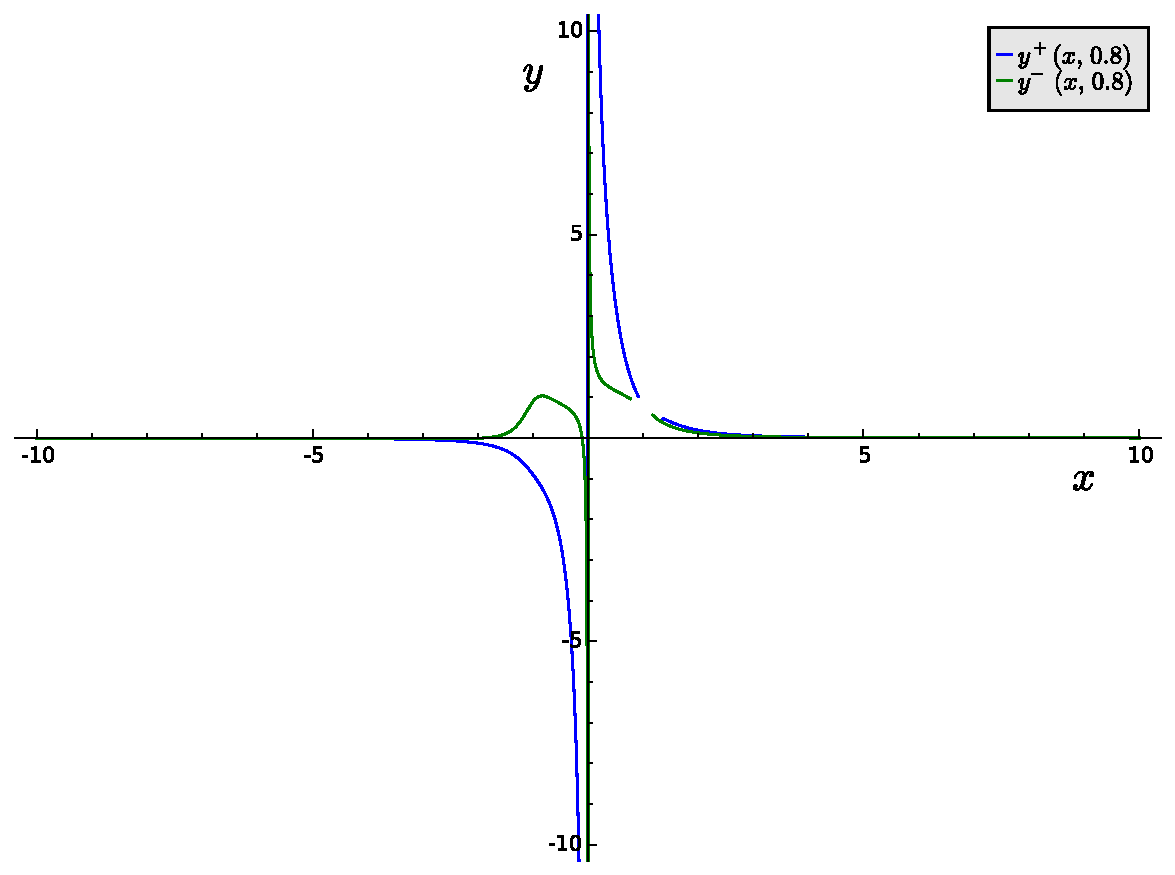
\includegraphics[width=1\textwidth]{plots/ch1_06_sols.pdf}
\caption{$y^+(x,v)$ and $y^-(x,v)$ for $v:= 0.8$.\label{fig:plotYs_1}}
\end{figure}
\begin{figure}[h]
\centering
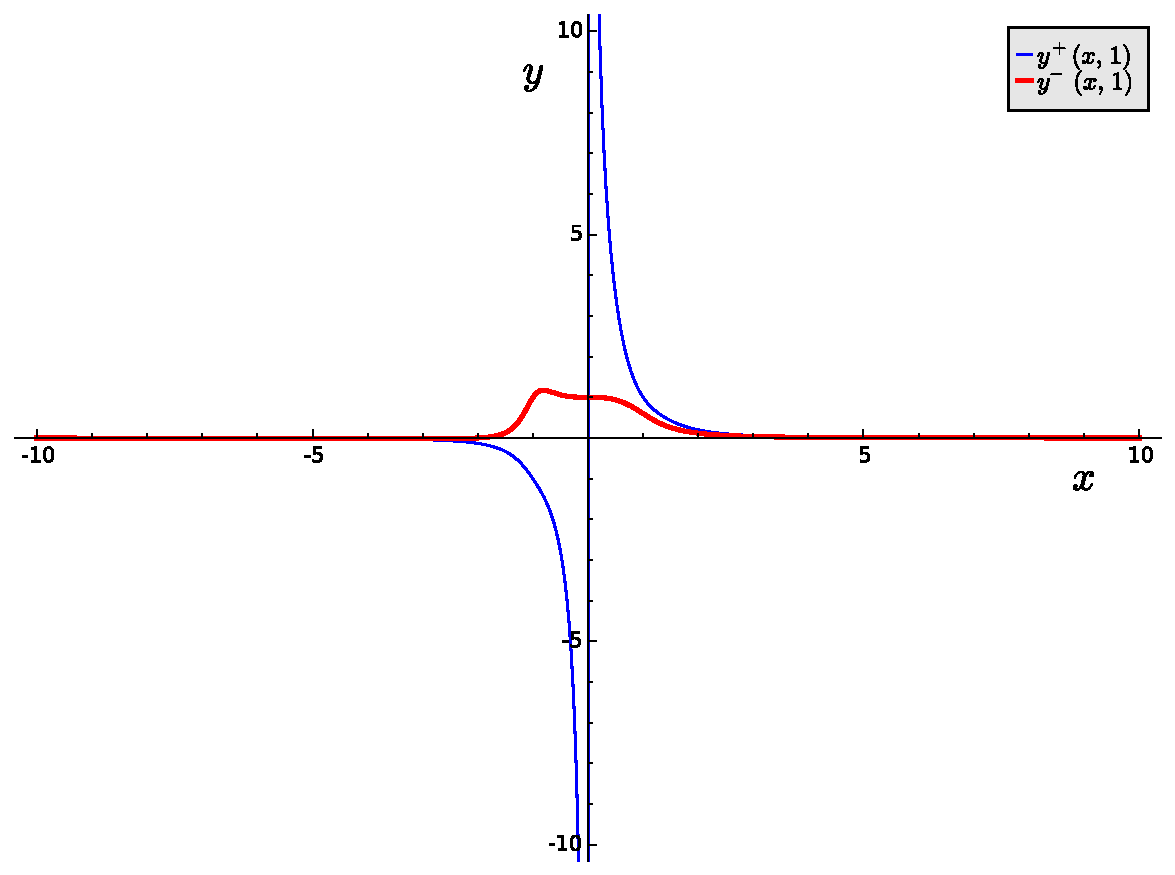
\includegraphics[width=1\textwidth]{plots/ch1_07_sols_1.pdf}
\caption{$y^+(x,v)$ and $y^-(x,v)$ for $v:=1$.\label{fig:plotYs_2}}
\end{figure}

The common domain of these two functions is the set 
$$
D_v:=\{x\in R:\, \Delta(x,v)\geq 0,\,x\neq 0\}.
$$ 
Notice that the only real root of the denominator is $x_0:=0$.\footnote{We checked with Laguerre's method, implemented with Python 2.7, that the polynomial $x^7+2x^4+x^3+x$ has 6 complex roots.} Let
$$
\gamma_v^+: D_v\to\R,\, x\mapsto\F(x,y^+(x,v))\quad\text{ and }\quad\gamma_v^-:D_v\to\R,\, x\mapsto\F(x,y^-(x,v))
$$
Note that $\F(\set{\G=v})=\text{im}(\gamma_v^+)\cup\text{im}(\gamma_v^-)$, so all reduce to prove the inclusion 
$$
(0,+\infty)\subset\text{im}(\gamma_v^+)\cup\text{im}(\gamma_v^-).
$$
\begin{center}
\fbox{\textbf{Step 2}} \emph{Main properties of $\gamma_v^+ \text{ and } \gamma_v^-$.}
\end{center}\label{step2}
In this section we are going to prove that:
$$
\text{(i)} \lim_{x\rightarrow \pm\infty}\gamma_v^+(x)=\lim_{x\rightarrow \pm\infty}\gamma_v^-(x)=0.
$$
$$\text{(ii)} \lim_{x\rightarrow 0}\gamma_v^+(x)=+\infty
,\quad \lim_{x\rightarrow 0}\gamma_v^-(x)=\left\{\begin{array}{ll}
+\infty&\text{ for $v\neq 1$}\\
 4 & \text{ for $v=1$}
\end{array} \right.
$$
Using Sage we can symbolically check how $\gamma_v^+\text{ and }\gamma_v^-$ look like, getting polynomials $A_1,A_2,B_1,B_2\in\R[x,v]$ and $C\in \R[x]$ such that:
$$\text{(a) }\gamma_v^+(x)=\dfrac{A_1(x,v)+B_1(x,v)\sqrt{\Delta(x,v)}}{C(x)}, \ \ 
\gamma_v^-(x)=\dfrac{A_2(x,v)+B_2(x,v)\sqrt{\Delta(x,v)}}{C(x)},$$
$$
\text{(b)}\ \ 
\arraycolsep=1.4pt\def\arraystretch{1.5}
\begin{array}{cclrl}
A_1(x,v)&=&\ \ A_2(x,v)\, , & \text{deg}_x(A_1)=\text{deg}_x(A_2)=24& \\
B_1(x,v)&=&-B_2(x,v)\, , &\text{deg}_x(B_1)=\text{deg}_x(B_2)=21& \\
C(x)&=&x^2(x^2+(x^3+1)^2)^4\, , & \text{deg}_x(C)=26&.
\end{array}
$$
We proceed to study $\gamma_v^+$ and $\gamma_v^-$ at the origin. Since $\Delta$ has even degree and positive leading coefficient with respect to $x$, it is positive for $\abs{x}$ large enough, so (i) holds.
			
Now, for $x=0$, we get $\Delta(0,v)=v>0$, thus $0\in\overline{D_v}$. Also:
\begin{itemize}
\item $A_1(0,v)+B_1(0,v) \sqrt{\Delta(0,v)}= v(1+\sqrt{v})^2>0$.
				\item $A_2(0,v)+B_2(0,v)\sqrt{\Delta(0,v)}=v(1-\sqrt{v})^2\geq 0$, and equality holds if and only if $v=1$.
\end{itemize}
			
\begin{figure}[h]
\centering
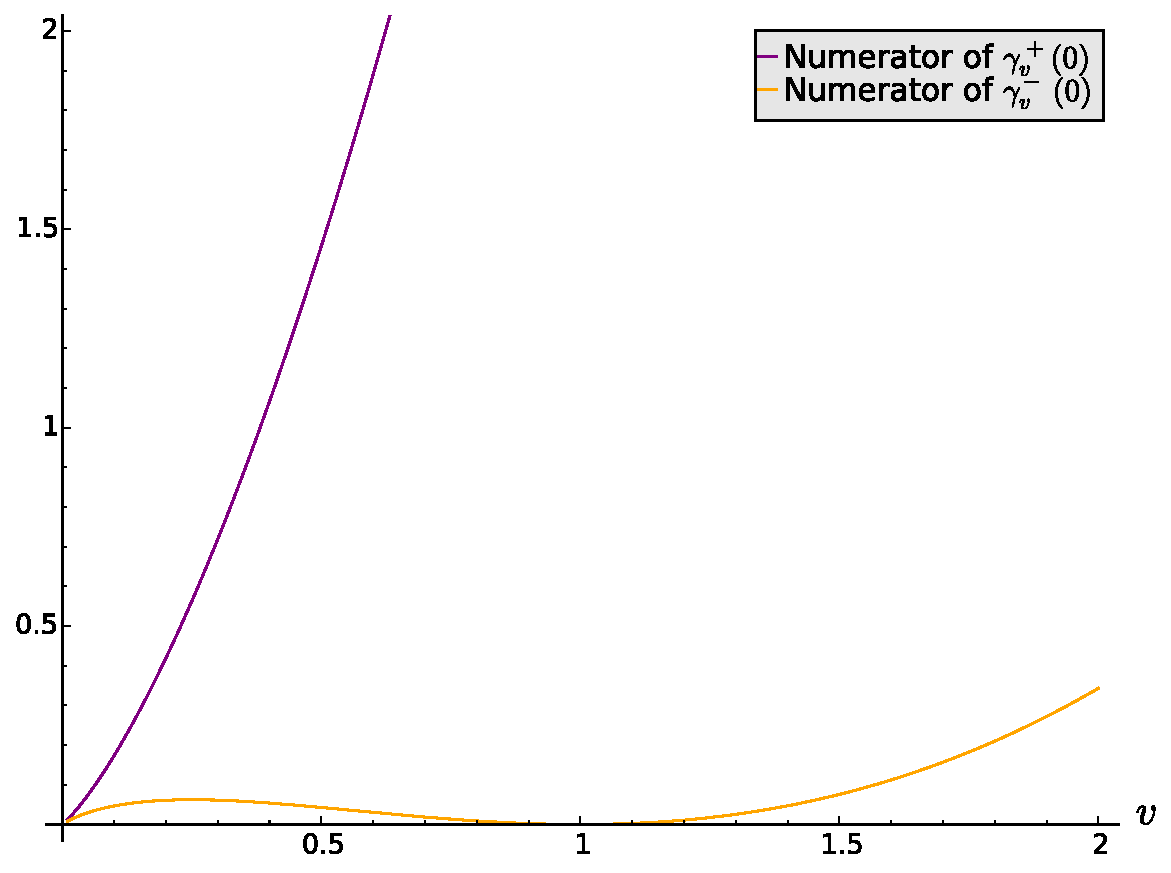
\includegraphics[width=0.75\textwidth]{plots/ch1_08_numerators.pdf}
\caption{Numerators of $\gamma_v^+$ and $\gamma_v^-$ for $x:=0$.\label{fig:numerators}}
\end{figure}
			
Thus, (ii) holds (we also checked it with Sage). The result for $v:=1$ in (ii) is not relevant here (see figure \ref{fig:limit}).
\begin{figure}[h]
\centering
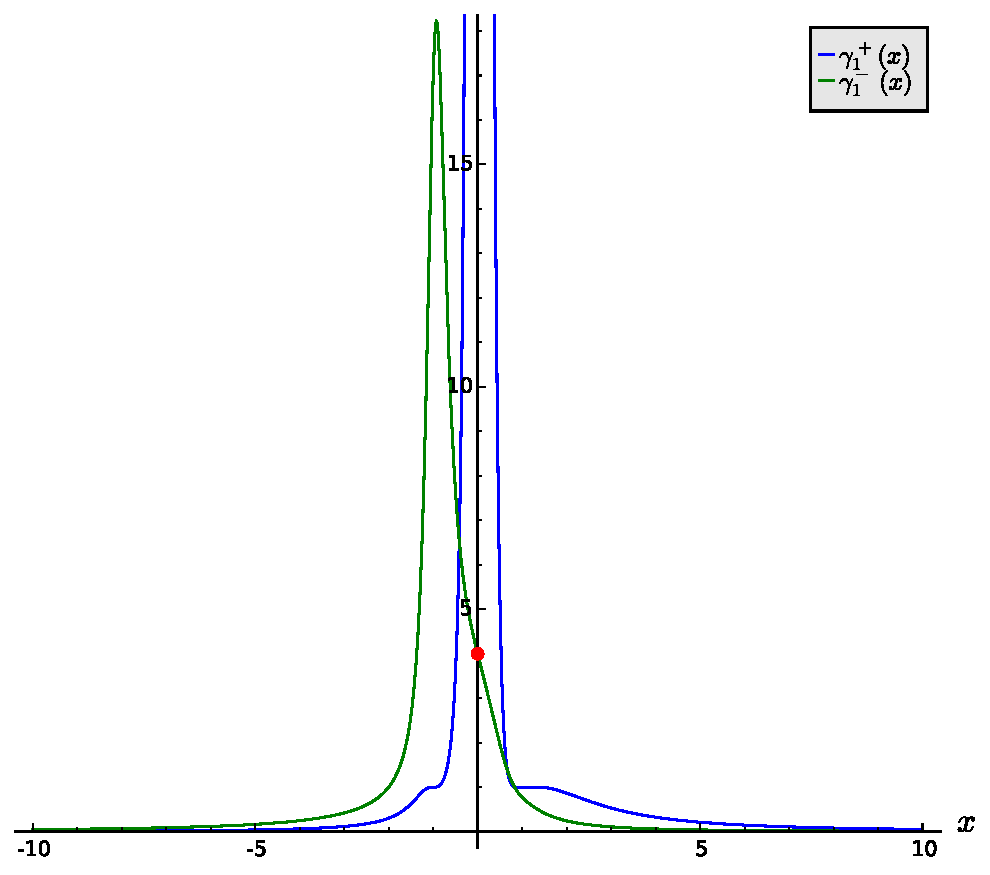
\includegraphics[width=1\textwidth]{plots/ch1_09_limit.pdf}
\caption{Notice the value of $\gamma_1^-(x)$ at $x=0$.\label{fig:limit}}
\end{figure}

\begin{center}
\fbox{\textbf{Step 3}} \emph{When $v\geq 0.28^2$ we have} $(0,+\infty)\subset\text{im}(\gamma_v^+)$.
\end{center}\label{step3}
In order to see whether $(0,+\infty)\subset\text{im}(\gamma_v^+)\cup\text{im}(\gamma_v^-)$ or not we are now going to study the domain $D_v$. To that end we need to study when $\Delta(x,v)=0$, so it seems convenient to define:
$$
v(x):=\frac{x^2(x+1)^2}{x^2+(x^3+1)^2},
$$
whose graph can be seen in figure \ref{fig:v(x)}. If $x\in(-\infty,0)$ we checked using Laguerre's method that the polynomial
\begin{figure}[h]\hspace{-0.2cm}
\begin{subfigure}{.5\linewidth}\centering
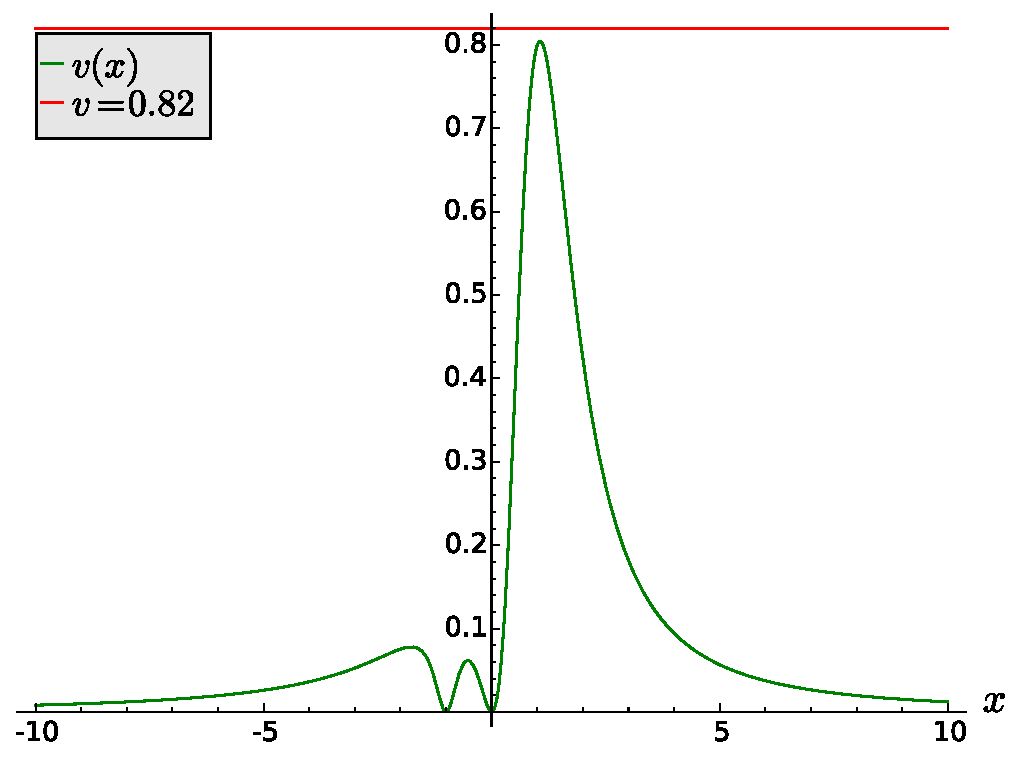
\includegraphics[width=1\textwidth]{plots/ch1_10_uve.pdf}
\caption{Plot of $v(x)$.\label{fig:uve}}
\end{subfigure}
\begin{subfigure}{.5\linewidth}\centering
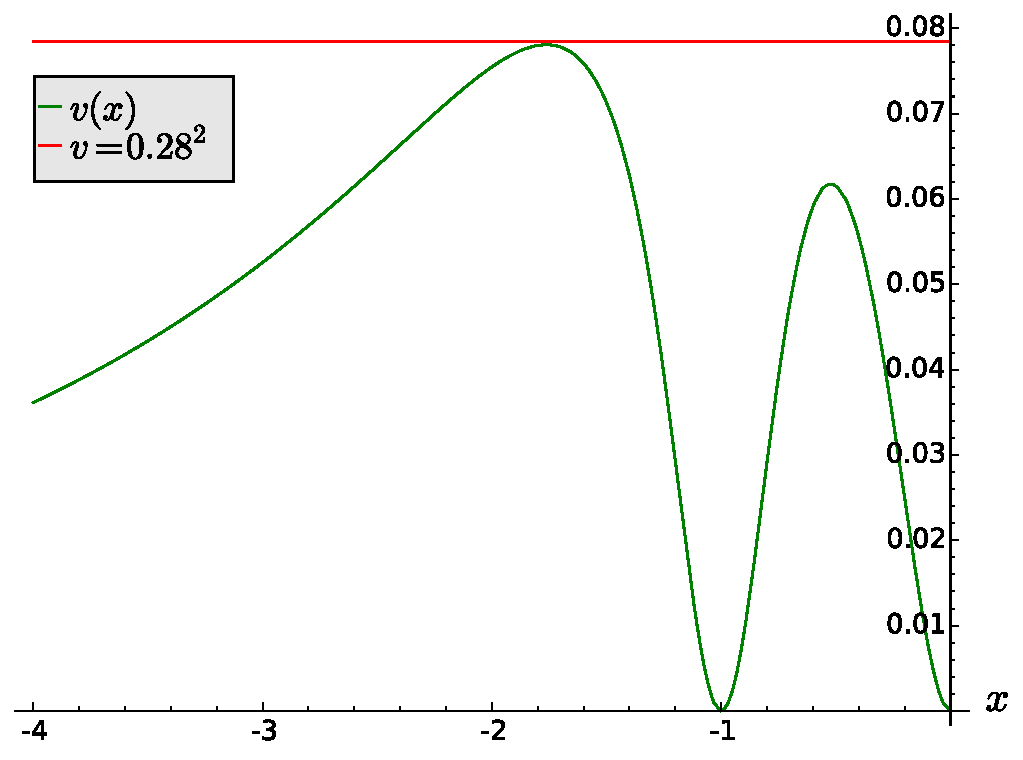
\includegraphics[width=1\textwidth]{plots/ch1_11_uve_detail.pdf}
\caption{Detail of the function when $x\in(-4,0)$.\label{fig:uveDetail}}
\end{subfigure}\\[1ex]
\caption{Plot of the univariate function $v(x)$.\label{fig:v(x)}}
\end{figure}
$$
\Delta(x,0.28^2)=0.0784\,x^{6}-x^{4}-1.8432\,x^{3}-0.9216\,x^{2}+0.0784
$$ 
has 4 complex roots and 2 real ones\footnote{The value $v_0:=0.28^2$ comes from a careful observation of the plot from figure \ref{fig:uveDetail}.}. These last are $\delta_0\approx 0.236$ and $\delta_1\approx 4.336$. Thus $\Delta({\tt x},v)$ has no negative roots for $v\ge 0.28^2$ and, in addition, it only attains positive values. Therefore $(-\infty,0)\subset D_v$. But then, as $\gamma_v^+$ is continuous and recalling the limits computed in \hyperref[step2]{Step 2}, we get  
$$
(0,+\infty)\subset\text{im}(\gamma_v^+)\subset\text{im}(\gamma_v^+)\cup\text{im}(\gamma_v^-).
$$
\begin{center}
\fbox{\textbf{Step 4}} \emph{When $0<v<0.28^2$ we have} $(0,+\infty)\subset\text{im}(\gamma_v^-)$.
\end{center}
\label{step4}
To prove that for $0<v<0.28^2$ the inclusion $(0,+\infty)\subset\text{im}(\gamma_v^-)$ holds it is enough to prove the existence of $N_v,\delta_v\in\R$ satisfying			
\begin{equation*}\qquad \quad
\qquad\quad\boxed{N_v<\delta_v,\ \ (-\infty,N_v]\cup[\delta_v,+\infty)\subset D_v\text{ and } \gamma_v^-(N_v)>\gamma_v^+(\delta_v)\\
}\qquad \qquad (\spadesuit)
\end{equation*}
\begin{figure}[h]
\centering
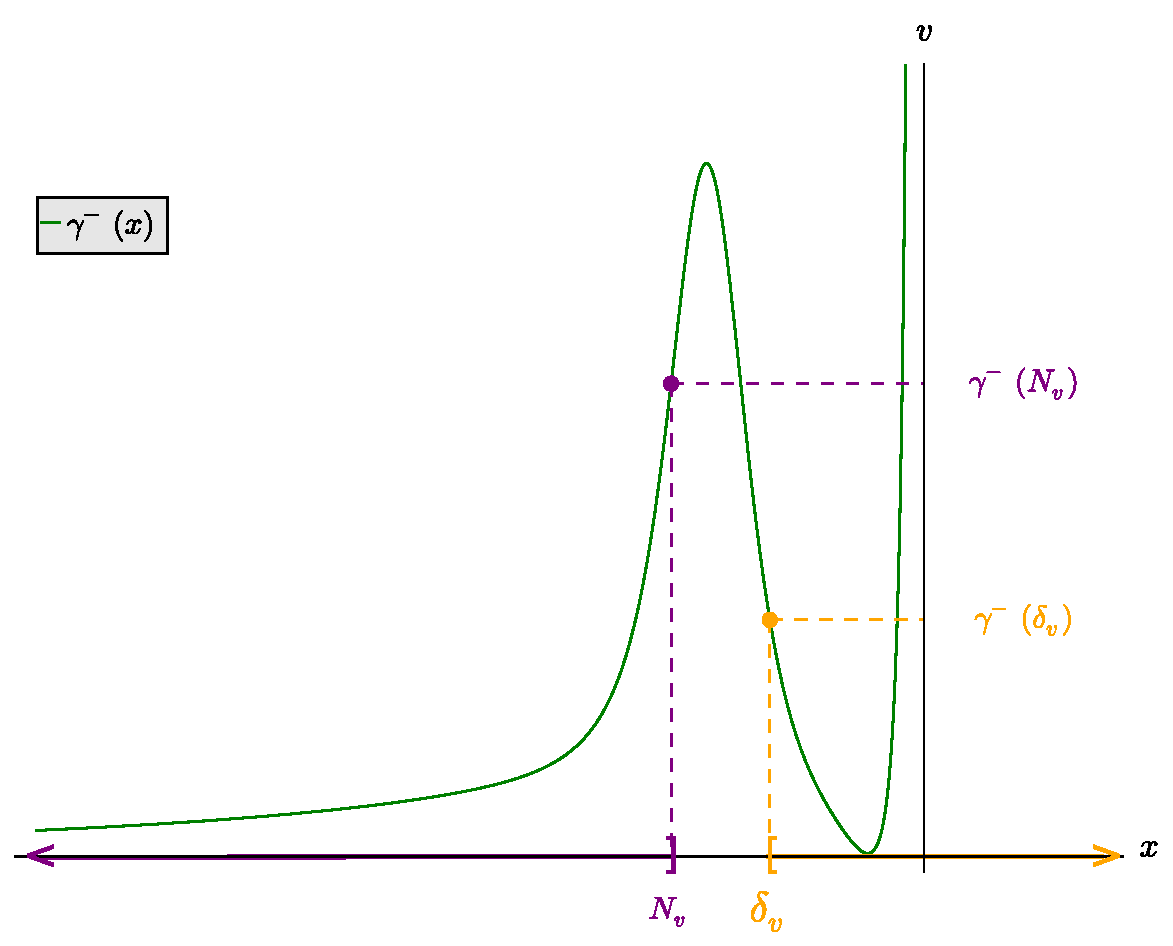
\includegraphics[width=1\textwidth]{plots/ch1_12_idea.pdf}
\caption{Idea of what we are saying with $(\spadesuit)$. Here $v:=0.1$.\label{fig:idea}}
\end{figure}
See figure \ref{fig:idea} to get an idea of what we are saying here. 

To prove the existence of such $N_v$ and $\delta_v$, we must compute the roots of $\Delta_v({\tt x})$ in an algebraic closure of the field of rational functions $\R(v)$. Such an algebraic closure is the field of Puiseux series $\C\left(\set{v^*}\right)$, see \ref{puiseux}. These roots are power series in $\C\left(\set{w^*}\right)$ with $w:=\sqrt{v}$, and we consider the largest and the smallest negative roots $\eta_v,\xi_v\in\R\left(\set{v^*}\right)$ of $\Delta_v$ with respect to the unique ordering in $\R\left(\set{v^*}\right)$ that makes $v$ positive and infinitesimal with respect to $\R$. These roots are:
			
\begin{equation*}\left\{\begin{split}
\eta_v:=&-\frac{1}{w}+1+w+w^2+\frac{5}{2}w^3+\cdots\\
\xi_v:=&-w-w^2-\frac{5}{2}w^3-6w^4+\cdots
\end{split}\right.
\end{equation*}
Notice that, by the definition of the ordering in $\R\left(\set{v^*}\right)$, the first coefficient of a series is the ``most meaningful orderwise". In particular $\eta_v<\xi_v$. To perform calculations, we handle suitable truncations of the involved series. Here the word suitable means ``as short as possible but order preserving"; in other words, we look for $N_v$ and $\delta_v$ with $N_v<\eta_v<\xi_v<\delta_v$, and in fact we choose
\begin{equation*}\left\{
\begin{split}
N_v:=&-\frac{1}{w}+1+w+w^2=\eta_v-\Big(\frac{5}{2}w^3+\cdots\Big)<\eta_v\\
\delta_v:=&-w-w^2-\frac{5}{2}w^3=\xi_v-(-6w^4+\cdots)>\xi_v
\end{split}\right.
\end{equation*}
We checked with Sage that $-\infty<N_v<\delta_v<0$ for $v\in (0,0.28^2)$ that is, for $w\in(0,0.28)$, see Figure \ref{fig:comp}. Now we can focus on proving $(\spadesuit)$. Since $\Delta(N_{w^2},w^2)$ and $\Delta(\delta_{w^2},w^2)$ are positive (see Figure \ref{fig:positive}) for $w\in (0,0.28)$, we get that $N_v, \delta_v\in D_v$.
\begin{figure}[h]\hspace{-0.25cm}
\begin{subfigure}{.50\linewidth}\centering
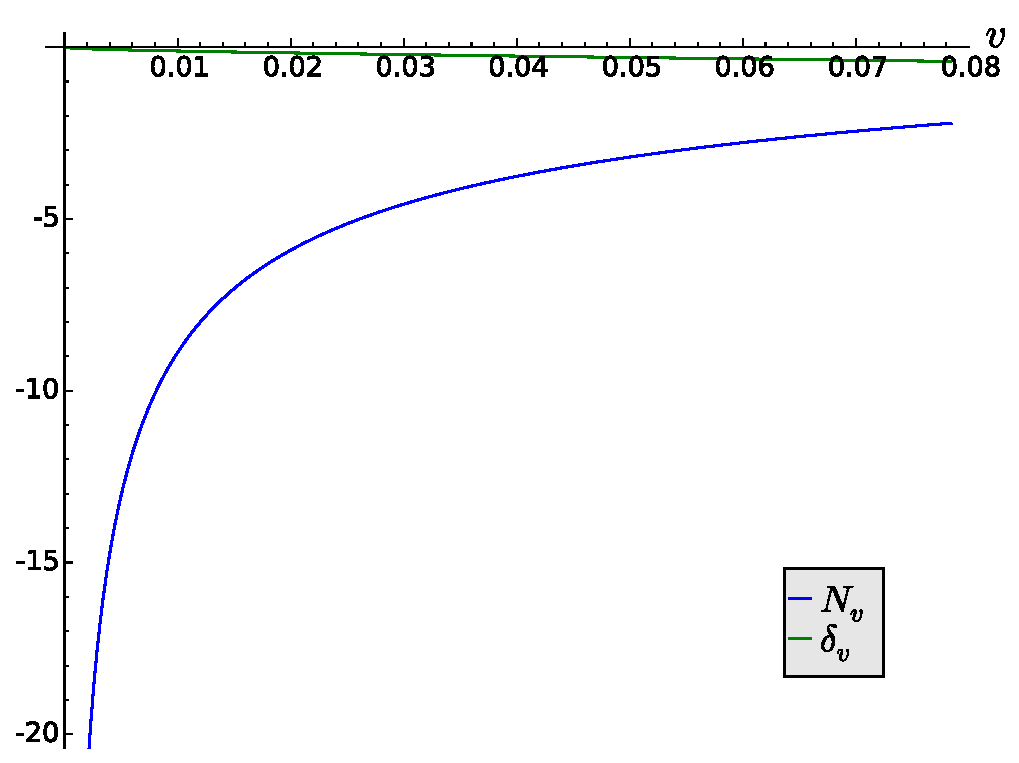
\includegraphics[width=1\textwidth]{plots/ch1_13_comp.pdf}
\caption{$-\infty<N_v<\delta_v<0$.\label{fig:comp}}
\end{subfigure}
\begin{subfigure}{.50\linewidth}\centering
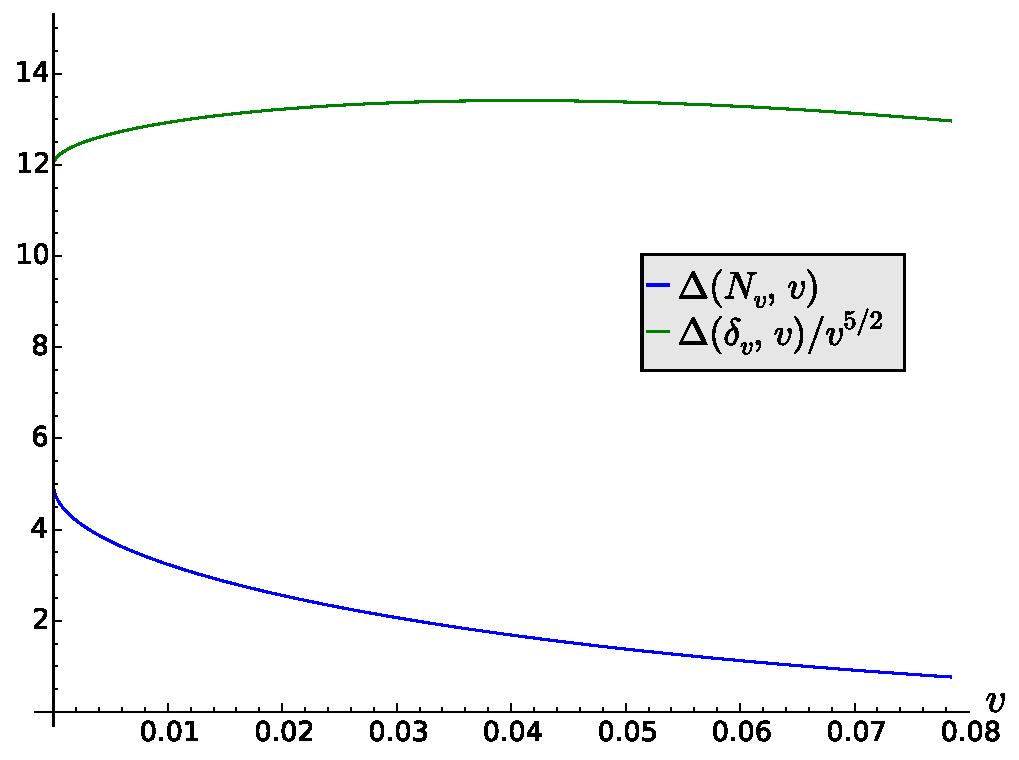
\includegraphics[width=1\textwidth]{plots/ch1_14_positive.pdf}
\caption{$\Delta(N_{v}, v), \Delta(\delta_{v},v) > 0$.\label{fig:positive}}
\end{subfigure}\\[1ex]
\caption{Plots of $N_v,\delta_v<0$ and $\Delta(N_{v},v),\ \Delta(\delta_{v},v)>0$ for $v\in(0, 0.28^2)$.\label{fig:N_delta}}
\end{figure} For the first part, let 
$$
D:=\bigcup_{v>0}D_v=\bigcup_{v>0}\set{x\in\R:\Delta(x,v)\geq 0,\,x\neq 0},
$$ 
whose boundary is the union of the axis $\{x=0\}\subset\R^2$ and the curve given by the equation $\Delta(x,v)=0$, that is, the graph of the regular function
$$
v(x)=\frac{x^2(x+1)^2}{x^2+(x^3+1)^2}.
$$
This graph is above the axis $\{v=0\}\subset R^2$. Then, $(-\infty,N_v]$ and $[\delta_v,0)$ are contained in the interior of $D_v$ for $v\in (0, 0.28^2)$, because the curves 
$$
\set{(\delta_v,v):0<v<0.28^2}\, \, \, \text{and}\, \, \, \set{(N_v,v):0<v<0.28^2}
$$ 
are contained in $D$, they are graphs above the vertical axis $\{x=0\}\subset R^2$, and $\delta_v<\xi_v$ and $N_v<\eta_v$ as we saw before. Look at figure \ref{fig:nice_plot}.

\begin{figure}[h]
\centering
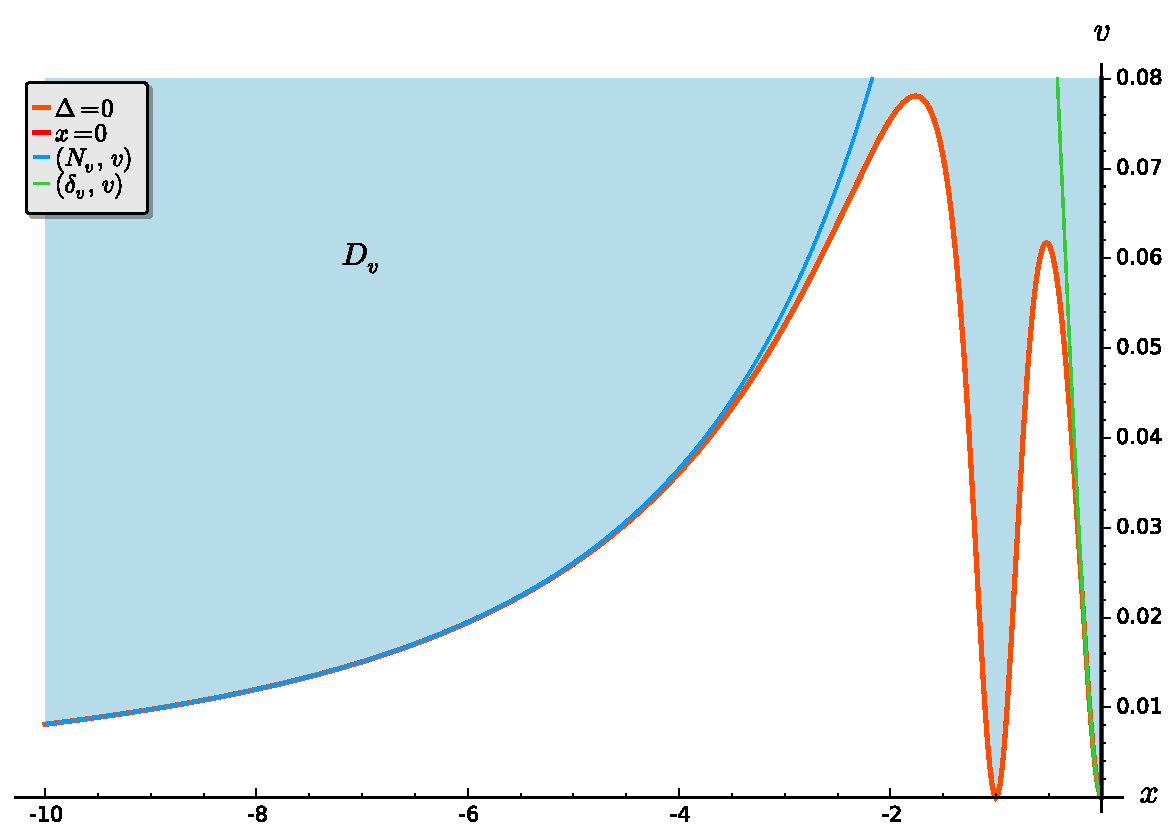
\includegraphics[width=1\textwidth]{plots/ch1_15_nice_plot.pdf}
\caption{Plot of $\set{(N_v,v)}, \set{(\delta_v,v)}\subset D_v$, for $0<v<0.28^2$.\label{fig:nice_plot}}
\end{figure}

\vspace{1mm}

So the only thing left to do is checking that $\gamma_v^-(N_v)>\gamma_v^-(\delta_v)$. Recall that 
$$
\gamma_v^-({\tt x})=\dfrac{A_2({\tt x},v)+B_2({\tt x},v)\sqrt{\Delta({\tt x},v)}}{C({\tt x})},
$$
with $\text{deg}_{\tt x}(A_2)=24,\, \, \text{deg}_{\tt x}(B_2)=21,\, \, \text{deg}_{\tt x}(\Delta)=6\, \, \text{ and }\text{deg}_{\tt x}(C)=26$. Consider:
$$
\arraycolsep=2pt\def\arraystretch{1.5}
\begin{array}{rclcrcl}
\cdot\ f_1(w)&=&A_2(N_{w^2},w^2)\cdot w^{24}& \qquad &\cdot\ f_2(w)&=& A_2(\delta_{w^2},w^2)\\
\cdot\ g_1(w)&=&B_2(N_{w^2},w^2)\cdot w^{21}& \qquad &\cdot\ g_2(w)&=&B_2(\delta_{w^2},w^2)\\
\cdot\ q_1(w)&=&\Delta(N_{w^2},w^2)& \qquad &\cdot\ q_2(w)&=&\Delta(\delta_{w^2},w^2)\\
\cdot\ h_1(w)&=&C(N_{w^2})\cdot w^{26}& \qquad &\cdot\ h_2(w)&=&C(\delta_{w^2}).
\end{array}
$$
Thus, we need to prove that for $w\in(0,0.28)$:
$$
\frac{f_1\cdot(w^{24})^{-1}+g_1\cdot (w^{21})^{-1}\sqrt{q_1}}{h_1\cdot(w^{26})^{-1}}>\frac{f_2+g_2\sqrt{q_2}}{h_2} \iff
$$
$$
\frac{w^2h_2f_1-f_2h_1}{h_1h_2}+\frac{w^5g_1\sqrt{q_1}}{h_1}-\frac{g_2\sqrt{q_2}}{h_2}>0,
$$
and we are going to prove that 
$$
\Lambda_1:= \frac{w^2h_2f_1-f_2h_1}{h_1h_2},\, \, \, \Lambda_2:=\frac{w^5g_1\sqrt{q_1}}{h_1} \, \text{ and } \Lambda_3 := -\frac{g_2\sqrt{q_2}}{h_2}
$$
are positive in the given interval, which only contains positive values. As $q_1,q_2$ are positive, we can clear away $w^5$ and $\sqrt{q_1}$ from $\Lambda_2$, and $\sqrt{q_2}$ from $\Lambda_3$. Furthermore, the polynomial $C({\tt x})={\tt x}^2({\tt x}^2+({\tt x}^3+1)^2)^4>0$, so we can also remove $h_1$ and $h_2$ from $\Lambda_1,\Lambda_2, \Lambda_3$. Thus it suffices to see that
$$
L:=\frac{w^2h_2f_1-f_2h_1}{w^4},\quad g_1,\quad K:=-\frac{g_2}{w^3}
$$ 
are positive for $w\in(0,0.28)$.

\vspace{2cm}

As we see in the figures they indeed are. This has been also checked with Sturm algorithm and numerically with Sage. Thus, $(\spadesuit)$ holds and the result is proved.

\begin{center}
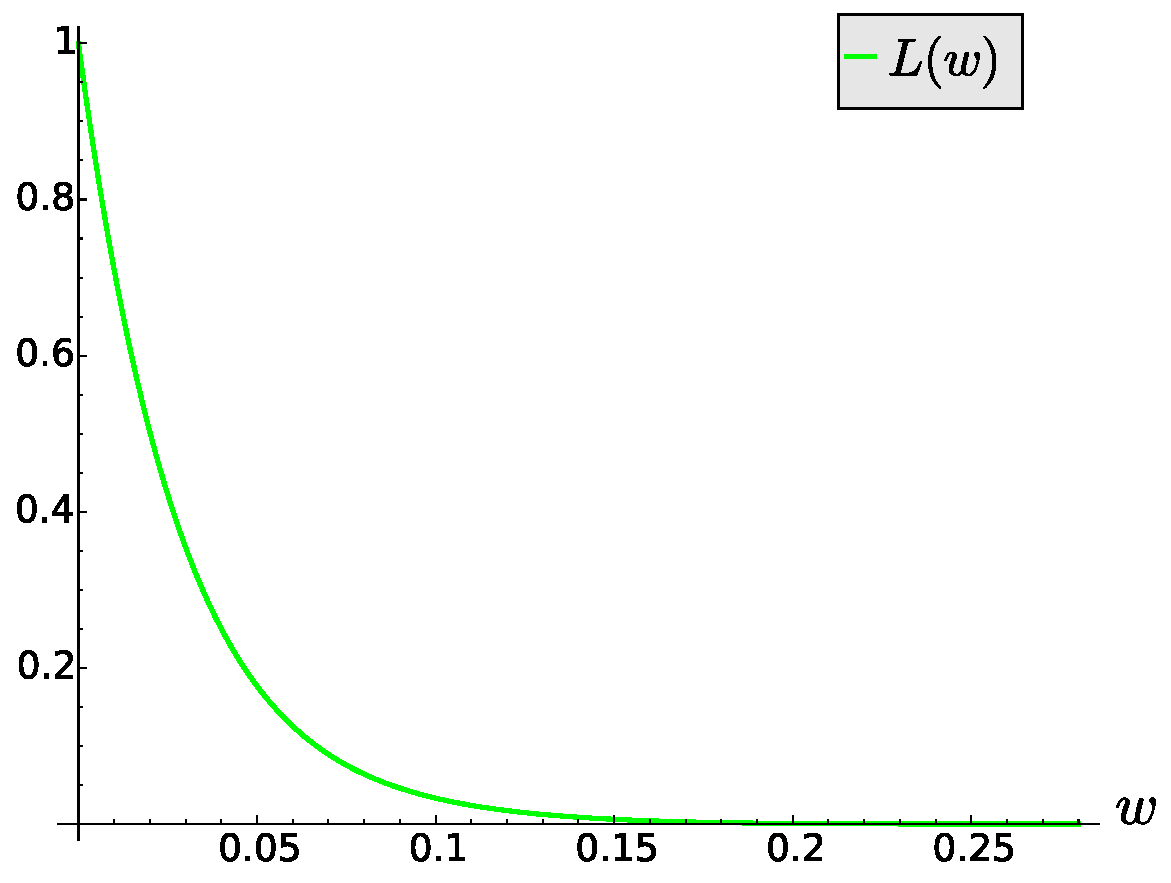
\includegraphics[width=0.45\linewidth]{plots/ch1_16_L.pdf}
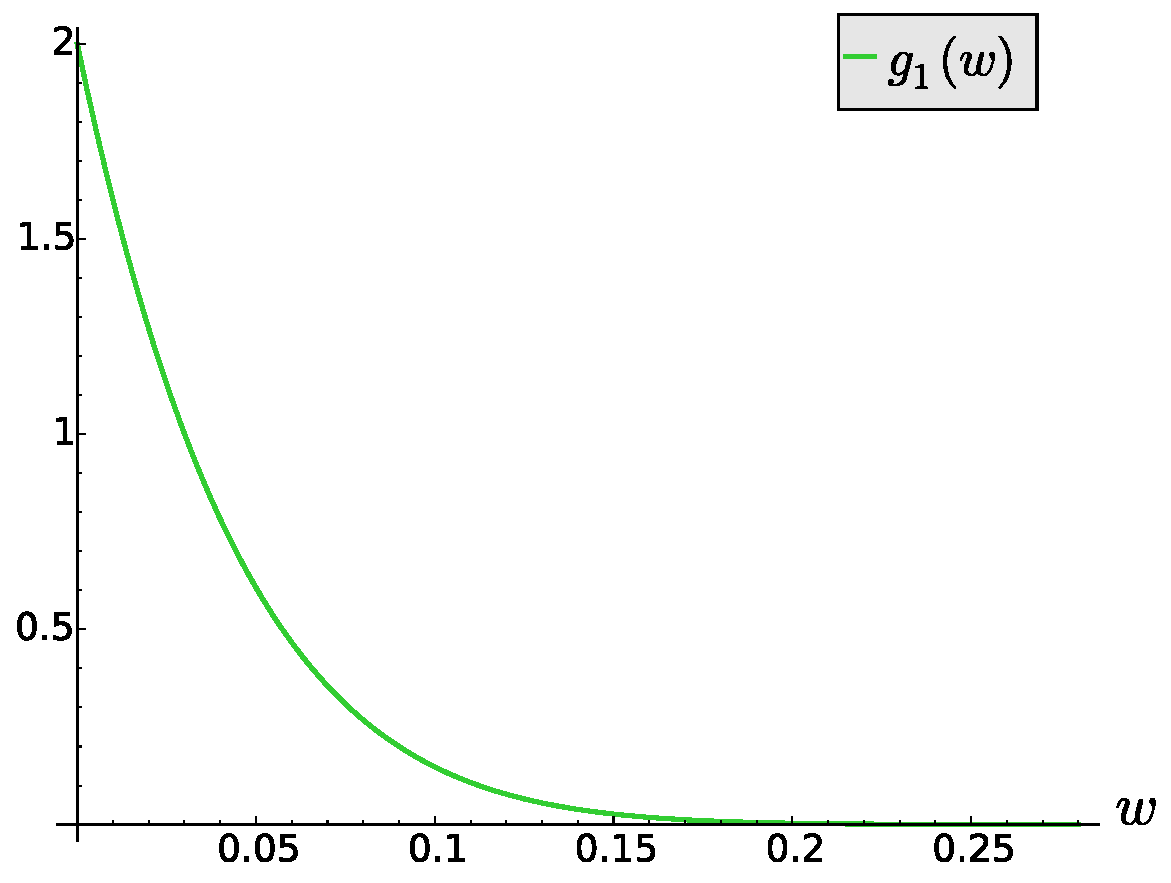
\includegraphics[width=0.45\linewidth]{plots/ch1_17_g_1.pdf} \\
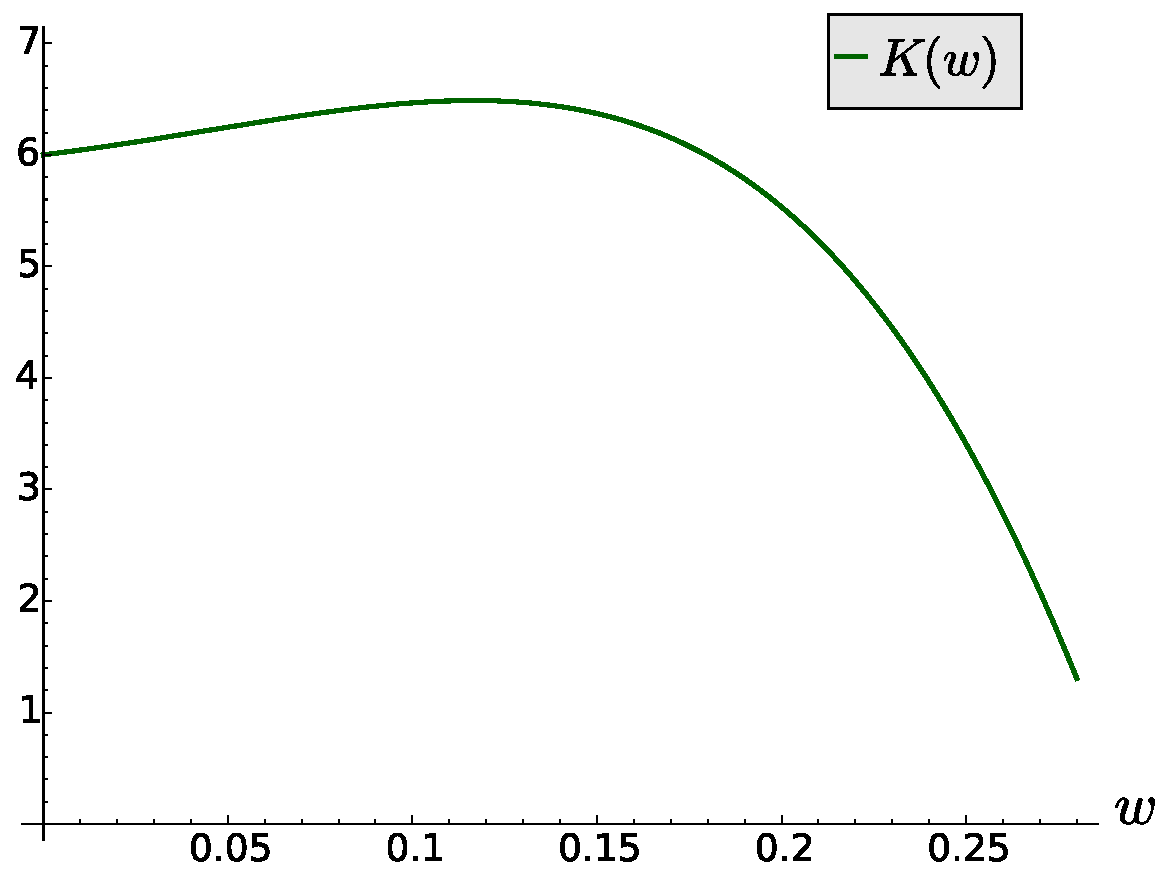
\includegraphics[width=0.45\linewidth]{plots/ch1_18_K.pdf}		
\end{center}
\qed
\end{section}
\end{chapter}

\begin{chapter}{A short proof for the open quadrant $\Qu$ problem}
\begin{section}{A new approach}
In the previous chapter, we proved that $\Qu$ is the image of $\R^2$ under the polynomial map $\P:=(\F,\G)$. This fact alongside Theorem \ref{finSetTh} were key for proving Theorem \ref{openQuadGen}. To achieve Theorem \ref{openQuad}, we needed the aid of a computer in order to check that certain polynomials do not have roots on particular intervals or that they are positive on them. Although legit, this procedure is controversial, and the authors kept on working on the problem of characterizing which semialgebraic subsets $\mathscr{S} \subset \R^m$ are polynomial images of $\R^n$ and wrote a new paper (\cite{fu}) with a much simpler proof.

In this third chapter we present a new approach to the open quadrant problem. We will show that $\Qu$ is the image of the composition of three simple polynomial maps: $\FF,\, \GG \text{ and } \HH$. The proof of Theorem \ref{openQuad} will be conducted by inspecting at the images of the aforementioned polynomials, albeit the lack of precise tools to determine the image of a polynomial map.

\begin{subsection}{The new polynomial maps}
In this subsection we introduce new polynomial maps that satisfy the requirements to prove Theorem \ref{openQuad} in a different way. To be more precise, we define 
$$
f:=\HH\circ\GG\circ\FF:\R^2\longrightarrow \R^2,
$$
where
\begin{equation*}
\boxed{
\begin{aligned}
\FF:\R^2\longrightarrow \R^2,\ (x,y)&\longmapsto((xy-1)^2+x^2,\ (xy-1)^2+y^2), \\
\GG:\R^2\longrightarrow \R^2,\ (x,y)&\longmapsto(x,\ y(xy-2)^2+x(xy-1)^2), \\
\HH:\R^2\longrightarrow \R^2,\ (x,y)&\longmapsto(x(xy-2)^2+\tfrac{1}{2}xy^2,\ y). \\
\end{aligned}
}
\end{equation*}
We can see how the graphs of the components of these maps look like in figure \ref{fig:ch2Maps}, and appreciate the symmetry between the $x$ and $y$ variables while the transformation is performed.

\vspace{1mm}

In the next section we proceed to develop the proof, which splits into three lemmas.

\begin{figure}
\hspace{-0.1cm}
\begin{subfigure}{.49\linewidth}\centering
\begin{tikzpicture}
\node[anchor=south west,inner sep=0] (img)at (0,0) {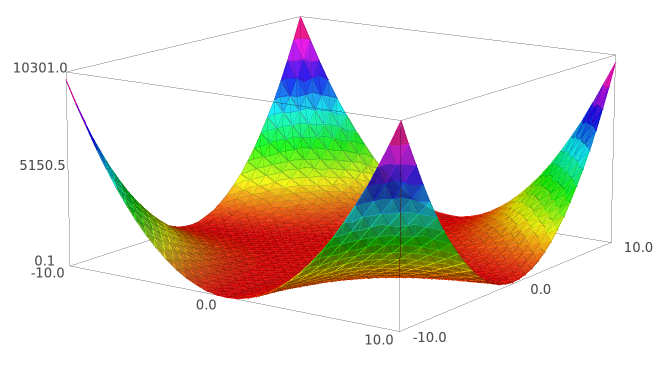
\includegraphics[width=1\textwidth]{plots/ch2_01_F_1.png}};
\path ($(img.north west)!0.28!(img.north east)$)|-coordinate(c1)($(img.south east)!0.1!(img.north east)$);
\path ($(img.north west)!0.85!(img.north east)$)|-coordinate(c2)($(img.south east)!0.15!(img.north east)$);
\draw (c1) node {$x$};
\draw (c2) node {$y$};
\end{tikzpicture}
\vspace{0.15cm}\caption{$\FF_1({\tt x},{\tt y})=({\tt x}{\tt y}-1)^2+{\tt x}^2$.\label{fig:FF_1}}
\end{subfigure}
\begin{subfigure}{.49\linewidth}\centering
\begin{tikzpicture}
\node[anchor=south west,inner sep=0] (img)at (0,0){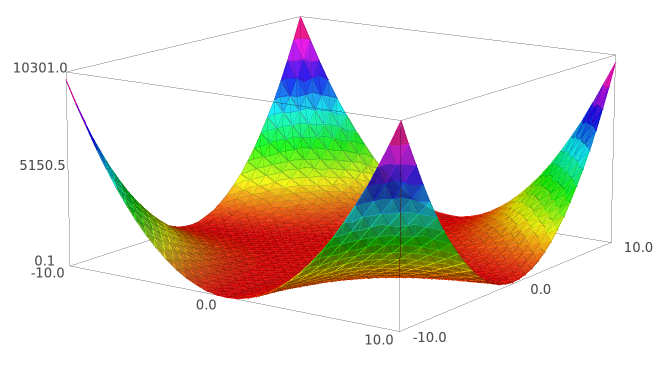
\includegraphics[width=1\textwidth]{plots/ch2_02_F_2.png}};
\path ($(img.north west)!0.28!(img.north east)$)|-coordinate(c1)($(img.south east)!0.1!(img.north east)$);
\path ($(img.north west)!0.85!(img.north east)$)|-coordinate(c2)($(img.south east)!0.15!(img.north east)$);
\draw (c1) node {$x$};
\draw (c2) node {$y$};
\end{tikzpicture}
\vspace{0.15cm}\caption{$\FF_2({\tt x},{\tt y})=({\tt x}{\tt y}-1)^2+{\tt y}^2$.\label{fig:FF_2}}
\end{subfigure}\\[1ex]
\vspace{0.4cm}
	
\hspace{-0.1cm}
\begin{subfigure}{.49\linewidth}\centering
\begin{tikzpicture}
\node[anchor=south west,inner sep=0] (img)at (0,0) {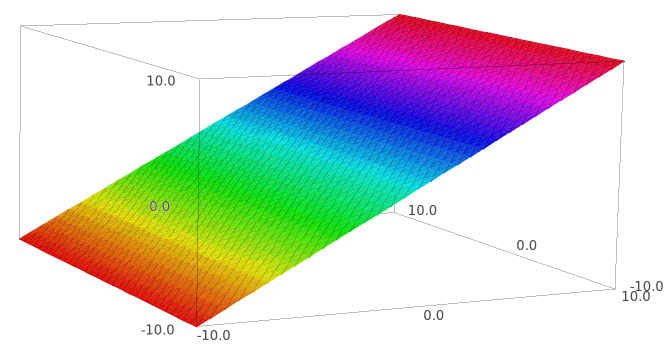
\includegraphics[width=1\textwidth]{plots/ch2_03_G_1.png}};
\path ($(img.north west)!0.67!(img.north east)$)|-coordinate(c1)($(img.south east)!0.055!(img.north east)$);
\path ($(img.north west)!0.72!(img.north east)$)|-coordinate(c2)($(img.south east)!0.26!(img.north east)$);
\draw (c1) node {$x$};
\draw (c2) node {$y$};
\end{tikzpicture}
\vspace{0.15cm}\caption{$\GG_1({\tt x}, {\tt y}) = {\tt x}$.\label{fig:GG_1}}
\end{subfigure}
\begin{subfigure}{.49\linewidth}\centering
\begin{tikzpicture}
\node[anchor=south west,inner sep=0] (img)at (0,0) {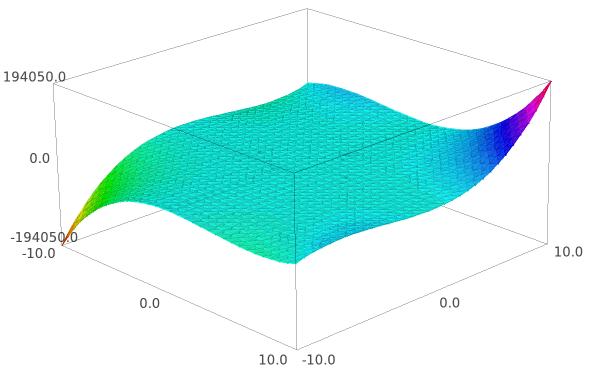
\includegraphics[width=1\textwidth]{plots/ch2_04_G_2.png}};
\path ($(img.north west)!0.2!(img.north east)$)|-coordinate(c1)($(img.south east)!0.15!(img.north east)$);
\path ($(img.north west)!0.81!(img.north east)$)|-coordinate(c2)($(img.south east)!0.14!(img.north east)$);
\draw (c1) node {$x$};
\draw (c2) node {$y$};
\end{tikzpicture}
\vspace{0.15cm}\caption{$\GG_2({\tt x},{\tt y})={\tt y}({\tt x}{\tt y}-2)^2+{\tt x}({\tt x}{\tt y}-1)^2$.\label{fig:GG_2}}
\end{subfigure}\\[1ex]
\vspace{0.4cm}

\hspace{-0.1cm}
\begin{subfigure}{.49\linewidth}\centering
\begin{tikzpicture}
\node[anchor=south west,inner sep=0] (img)at (0,0) {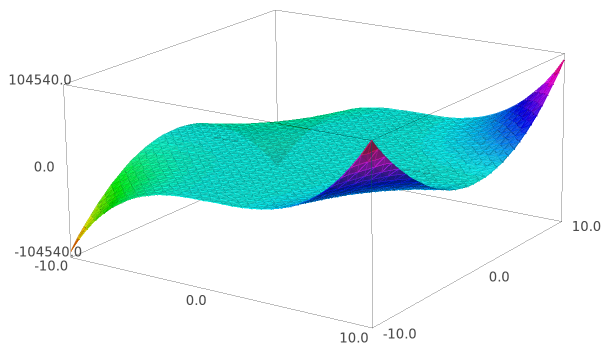
\includegraphics[width=1\textwidth]{plots/ch2_05_H_1.png}};
\path ($(img.north west)!0.29!(img.north east)$)|-coordinate(c1)($(img.south east)!0.08!(img.north east)$);
\path ($(img.north west)!0.85!(img.north east)$)|-coordinate(c2)($(img.south east)!0.14!(img.north east)$);
\draw (c1) node {$x$};
\draw (c2) node {$y$};
\end{tikzpicture}
\vspace{0.15cm}\caption{$\HH_1({\tt x},{\tt y})={\tt x}({\tt x}{\tt y}-2)^2+\tfrac{1}{2}{\tt x}{\tt y}^2$.\label{fig:HH_1}}
\end{subfigure}
\begin{subfigure}{.49\linewidth}\centering
\begin{tikzpicture}
\node[anchor=south west,inner sep=0] (img)at (0,0) {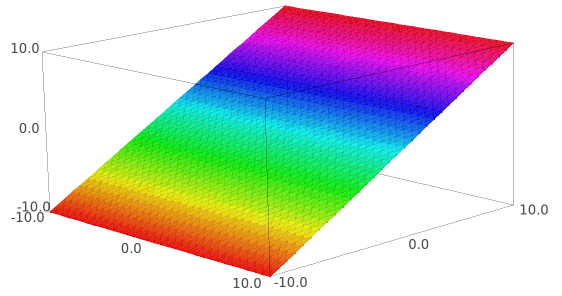
\includegraphics[width=1\textwidth]{plots/ch2_06_H_2.png}};
\path ($(img.north west)!0.2!(img.north east)$)|-coordinate(c1)($(img.south east)!0.1!(img.north east)$);
\path ($(img.north west)!0.78!(img.north east)$)|-coordinate(c2)($(img.south east)!0.11!(img.north east)$);
\draw (c1) node {$x$};
\draw (c2) node {$y$};
\end{tikzpicture}
\vspace{0.15cm}\caption{$\HH_2({\tt x},{\tt y})={\tt y}$.\label{fig:HH_2}}
\end{subfigure}
\vspace{0.7cm}\caption{The polynomial maps from the second proof: $(\HH\circ\GG\circ\FF)(\R^2)=\Qu$.\label{fig:ch2Maps}}
\end{figure}
\end{subsection}
\end{section}

\begin{section}{The new proof for the open quadrant problem}
As we have anticipated before, $\Qu$ is the image of the composition $\HH\circ\GG\circ \FF$, but before proving this fact we need three auxiliar lemmas in order to shed some light on the properties that the images of $\FF,\,\GG\text { and }\HH$ enjoy.

\begin{subsection}{The first lemma}
\begin{lemma}\label{lemma1} \em Let $\mathscr{A}:=\set{xy\ge1}\ \cap\, \Qu$. Then the image of the map
$$
\FF:=(\FF_1,\FF_2):\R^2\to\R^2,(x,y)\mapsto((xy-1)^2+x^2,(xy-1)^2+y^2)
$$
satisfies that $\mathscr{A}\subset\FF(\R^2)\subset\Qu$. \em 
\begin{Proof}
Since $\FF_1$ and $\FF_2$ are positive on $\R^2$, the inclusion $\FF(\R^2) \subset \Qu$ is evident. To prove the other inclusion, we must show that for $(a,b)\in\mathscr{A}$ the system of polynomial equations
\begin{equation}\label{eq:systemF}
\left\{
\begin{aligned}
({\tt x}{\tt y}-1)^2+{\tt x}^2=a\\
({\tt x}{\tt y}-1)^2+{\tt y}^2=b\\
\end{aligned}
\right.
\end{equation}
has a solution $(x_0,y_0)\in\R^2$. Set ${\tt z}:={\tt x}{\tt y}-1$ in order to rewrite the system \ref{eq:systemF} in terms of ${\tt x}$ and ${\tt z}$. Since ${\tt y}=\frac{{\tt z}+1}{{\tt x}}$ we get:
\begin{equation}\label{eq:system2F}
\left\{
\begin{aligned}
&{\tt z}^2+{\tt x}^2&=a\\
&{\tt z}^2+\frac{({\tt z}+1)^2}{{\tt x}^2}&=b&.\\
\end{aligned}
\right.
\end{equation}
By eliminating ${\tt x}$ on the system \ref{eq:system2F} we deduce that ${\tt z}$ must be a root of the polynomial
$$
P({\tt z}):={\tt z}^4-(a+b+1){\tt z}^2-2{\tt z}+(ab-1)=0.
$$
Taking into account that $(a,b)\in\mathscr{A}$ satisfy that $a,b>0$ and $ab\ge1$, we notice that $P$ is a monic polynomial of even degree satisfying
$$
P(0)=ab-1\ge0\quad\text{ and }\quad P(\sqrt{a})=-2\sqrt{a}-a-1<0.
$$
Thus, $P$ has a real root $z_0$ such that $0\le z_0<\sqrt{a}$, so we set:
$$
x_0:=\sqrt{a-z_0^2}\quad \text{ and } \quad y_0:= \frac{z_0+1}{x_0}.
$$
Then $F(x_0,y_0)=(a,b)$ and $\mathscr{A}\subset\FF(\R^2)$, as required.
\qed
\end{Proof}
\end{lemma}
\end{subsection}

\begin{figure}[h]
\begin{subfigure}{.5\linewidth}\centering
\begin{tikzpicture}
\node[anchor=south west,inner sep=0] (img)at (0,0) {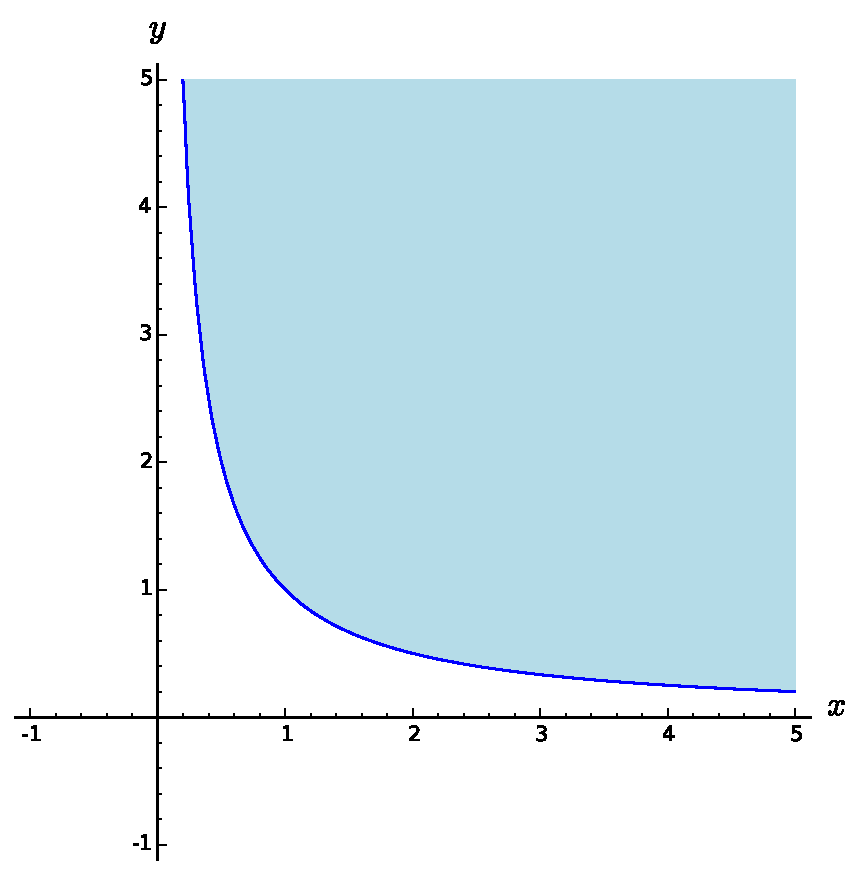
\includegraphics[width=1\textwidth]{plots/ch2_07_A.pdf}};
\path ($(img.north west)!0.6!(img.north east)$)|-coordinate(c1)($(img.south east)!0.7!(img.north east)$);% c1: lugar donde poner \mathscr{A}
\draw (c1) node {\huge{$\mathscr{A}$}};
\end{tikzpicture}
\caption{$\mathscr{A}=\set{xy\ge 1}\ \cap\, \Qu$.\label{fig:setA}}
\end{subfigure}
\hspace{-0.2cm}
\begin{subfigure}{.5\linewidth}\centering
\begin{tikzpicture}
\node[anchor=south west,inner sep=0] (img)at (0,0) {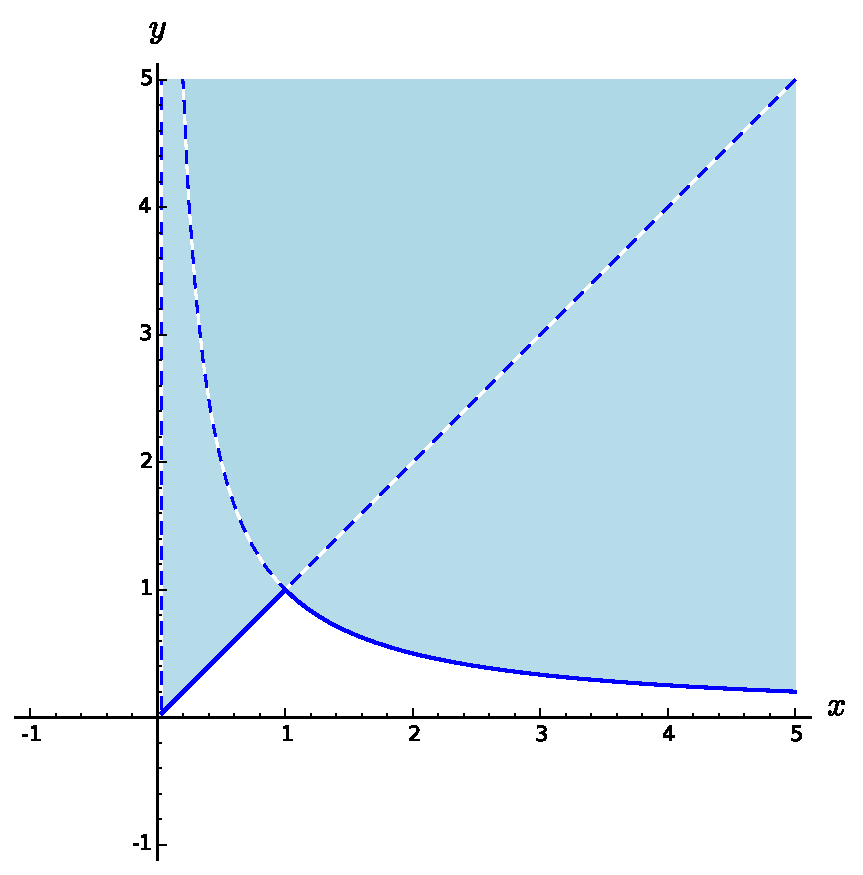
\includegraphics[width=1\textwidth]{plots/ch2_08_B.pdf}};
\path ($(img.north west)!0.6!(img.north east)$)|-coordinate(c1)($(img.south east)!0.7!(img.north east)$);% c1: lugar donde poner \mathscr{B}
\draw (c1) node {\huge{$\mathscr{B}$}};
\end{tikzpicture}
\caption{$\mathscr{B}=\mathscr{A}\cup\set{y\ge x>0}$.\label{fig:setB}}
\end{subfigure}
\caption{Relevant sets for Lemmas \ref{lemma1}, \ref{lemma2} and \ref{lemma3}.\label{fig:setsAB}}
\end{figure}

\begin{subsection}{The second lemma}
\begin{lemma}\label{lemma2} \em Let $\mathscr{B}:=\mathscr{A}\cup\set{y\ge x>0}$. Then, the map
$$
\GG:=(\GG_1,\GG_2):\R^2\to\R^2,(x,y)\mapsto (x,\ y(xy-2)^2+x(xy-1)^2)
$$
satisfies that $\mathscr{B}\subset\GG(\mathscr{A})\subset\GG(\Qu)\subset\Qu$. \em 
\begin{Proof}
The inclusion $\GG(\mathscr{A}) \subset \GG(\Qu)$ is trivial because $\mathscr{A}\subset\Qu$. The last inclusion $\GG(\Qu) \subset\Qu$ also holds since $\GG_1$ and $\GG_2$ are strictly positive on $\Qu$: if $x_0,y_0>0$ then $\GG_1(x_0,y_0)=x_0> 0$ and $\GG_2(x_0,y_0)=y_0(x_0y_0-2)^2+x_0(x_0y_0-1)^2>0$. Notice that $\GG_2(x_0,y_0)\ne0$. Otherwise there would exists a solution of the system of equations
\begin{equation*}
\left\{
\begin{aligned}
&{\tt x}{\tt y}-1=0\\
&{\tt x}{\tt y}-2=0,\\
\end{aligned}
\right.
\end{equation*}
which is not possible.

\vspace{1mm}

Now we can focus on proving $\mathscr{B} \subset \GG(\mathscr{A})$. First of all, notice that we can express the set $\mathscr{B}$ as a union of closed half-lines. Precisely, for each $x>0$ let $\mathscr{B}_x:=[y_x,+\infty)$, where $y_x:=\text{min}\set{x,1/x}$ and notice that
$$
\mathscr{B}=\bigsqcup_{x>0}(\set{x}\times\mathscr{B}_x).
$$
That is, we are ``slicing'' the set $\mathscr{B}$ vertically, depending on $x$. Now look at the definition of the polynomial $\GG_2$ and consider for each $x>0$ the polynomial $\phi_x\in\R[{\tt y}]$ (dependent on the variable ${\tt y})$:
$$
\phi_x({\tt y}):={\tt y}(x{\tt y}-2)^2+x(x{\tt y}-1)^2=x^2{\tt y}^3+(x^3-4x){\tt y}^2+(4-2x^2){\tt y}+x.
$$
The polynomials $\phi_x({\tt y})$ have odd degree and positive leading coefficient since $x > 0$. Now notice that if we fix $x_0 > 0$ then we get the following sequence of inclusions:
\begin{equation*}
\begin{aligned}
\phi_{x_0}(&[1/x_0,+\infty))\ \supset ^1 \ \phi_{x_0}([2/x_0,+\infty))\\
&\quad \quad \ \rotatebox[origin=c]{90}{$\subset$}\,^2 \hspace{3cm} \rotatebox[origin=c]{90}{$\subset$}\,^3\\
&[1/x_0,+\infty) \hspace{1.9cm}[x_0, +\infty) \\
\end{aligned}
\end{equation*}
Inclusion $^1$ follows from the fact that $[1/x_0, +\infty) \supset [2/x_0, +\infty)$ (notice that for $x>0$ the graph of the map $2/x$ is ``above'' the one of $1/x$). Inclusion $^2$ and $^3$ follow from the fact that $\phi_{x_0}({\tt y})$ has positive leading coefficient and the computation of the images of $1/x_0$ and $2/x_0$ through $\phi_{x_0}({\tt y})$:
\begin{equation*}
\begin{aligned}
\phi_{x_0}\left(\frac{1}{x_0}\right)&=\frac{1}{x_0}+\left((x_0^3-4x_0)\frac{1}{x_0^2}+(4-2x_0^2)\frac{1}{x_0}+x_0\right)= \frac{1}{x_0}\\
\phi_{x_0}\left(\frac{2}{x_0}\right)&=\left(\frac{8}{x_0}+(x_0^3-4x_0)\frac{4}{x_0^2}+(4-2x_0^2)\frac{2}{x_0}\right)+x_0= x_0.\\
\end{aligned}
\end{equation*}
Now it is clear that:
$$
\mathscr{B}_x=[y_x,+\infty)\subset\phi_x([1/x, +\infty)).
$$
Then we can prove the desired inclusion in this way:
$$
\mathscr{B}=\bigsqcup_{x>0}\big(\set{x}\times\mathscr{B}_x\big)\subset\bigsqcup_{x>0}\big(\set{x}\times\phi_x([1/x,+\infty))\big)=\bigsqcup_{x>0}\GG\big(\set{x}\times[1/x,+\infty)\big)=\GG(\mathscr{A}),
$$
which concludes the proof.
\qed
\end{Proof}
\end{lemma}
\end{subsection}

\begin{center}
\begin{figure}[h]
\begin{subfigure}{.49\linewidth}\centering
\begin{tikzpicture}
\node[anchor=south west,inner sep=0] (img)at (0,0) {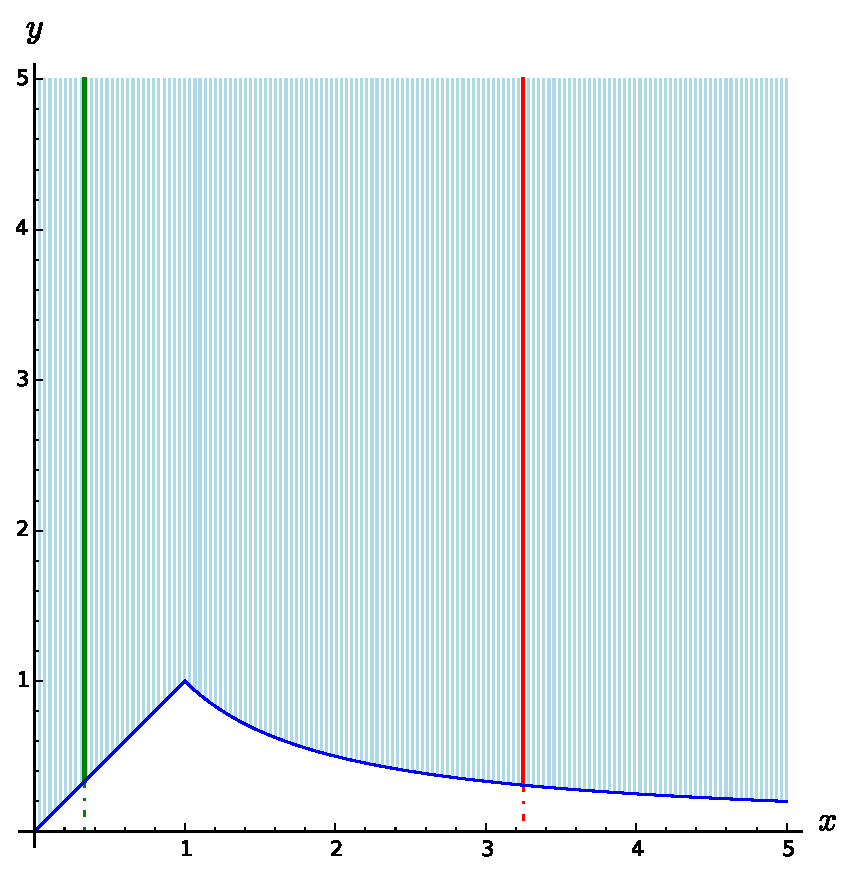
\includegraphics[width=1\textwidth]{plots/ch2_09_B_vert.pdf}};
\path ($(img.north west)!0.8!(img.north east)$)|-coordinate(c1)($(img.south east)!0.8!(img.north east)$); % Para \mathscr{B}
\path ($(img.north west)!0.1!(img.north east)$)|-coordinate(c2)($(img.south east)!0.89!(img.north east)$); % Para la flecha de x_0
\path ($(img.north west)!0.613!(img.north east)$)|-coordinate(c3)($(img.south east)!0.89!(img.north east)$); % Para la flecha de x_1
\path ($(img.north west)!0.1!(img.north east)$)|-coordinate(c4)($(img.south east)!0.105!(img.north east)$); % Para [
\path ($(img.north west)!0.613!(img.north east)$)|-coordinate(c5)($(img.south east)!0.101!(img.north east)$); % Para [
\path ($(img.north west)!0.1!(img.north east)$)|-coordinate(c6)($(img.south east)!0.01!(img.north east)$); % Para x_0
\path ($(img.north west)!0.613!(img.north east)$)|-coordinate(c7)($(img.south east)!0.01!(img.north east)$); % Para x_1
\path ($(img.north west)!0.26!(img.north east)$)|-coordinate(c8)($(img.south east)!0.55!(img.north east)$); % Para B_{x_0}
\path ($(img.north west)!0.77!(img.north east)$)|-coordinate(c9)($(img.south east)!0.35!(img.north east)$); % Para B_{x_1}
\draw (c1) node {\huge{$\mathscr{B}$}};
\draw (c2) node {\Large{\color[rgb]{0,0.392157,0}{$\uparrow$}}};
\draw (c3) node {\Large{\color[rgb]{1,0,0}{$\uparrow$}}};
\draw (c4) node {\large{\color[rgb]{0,0.392157,0}{\rotatebox[origin=c]{90}{[}}}};
\draw (c5) node {\large{\color[rgb]{1,0,0}{\rotatebox[origin=c]{90}{[}}}};
\draw (c6) node {\large{\color[rgb]{0,0.392157,0}{$x_0$}}};
\draw (c7) node {\large{\color[rgb]{1,0,0}{$x_1$}}};
\draw (c8) node {\large{\color[rgb]{0,0.392157,0}{$\set{x_0} \times \mathscr{B}_{x_0}$}}};
\draw (c9) node {\large{\color[rgb]{1,0,0}{$\set{x_1} \times \mathscr{B}_{x_1}$}}};
\end{tikzpicture}
\caption{$\mathscr{B} = \bigsqcup_{x>0}(\set{x} \times \mathscr{B}_{x})$.\label{fig:Bvert}}
\end{subfigure}
\begin{subfigure}{.49\linewidth}\centering
\begin{tikzpicture}
\node[anchor=south west,inner sep=0] (img)at (0,0) {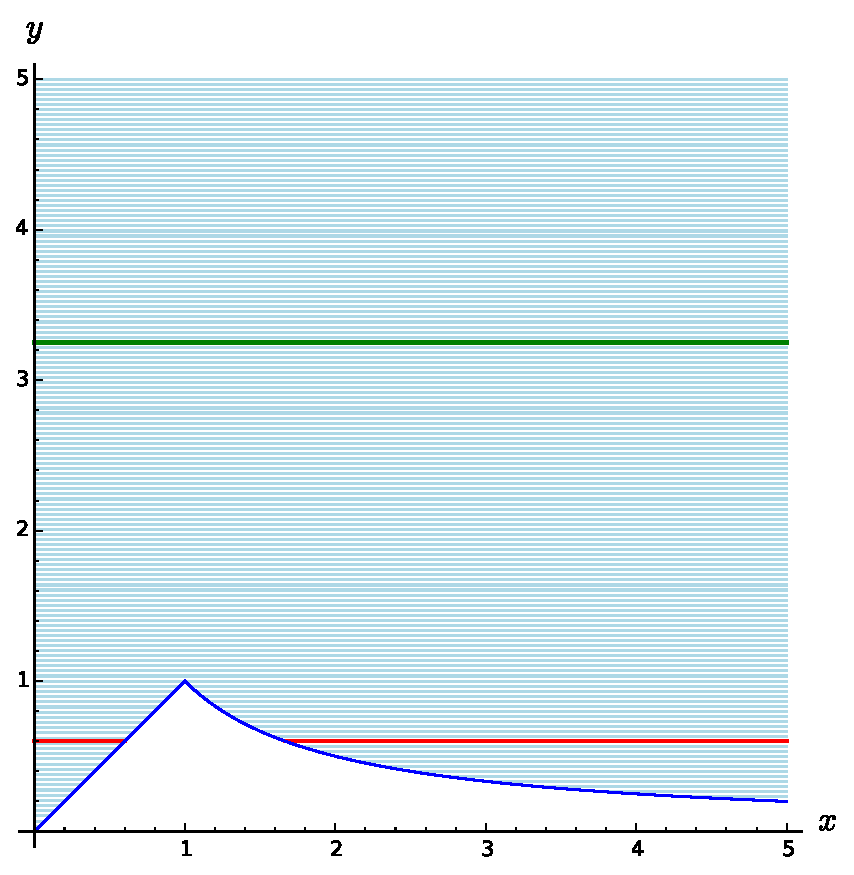
\includegraphics[width=1\textwidth]{plots/ch2_10_B_hor.pdf}};
\path ($(img.north west)!0.6!(img.north east)$)|-coordinate(c1)($(img.south east)!0.7!(img.north east)$);% c1: lugar donde poner \mathscr{B}
\path ($(img.north west)!0.8!(img.north east)$)|-coordinate(c1)($(img.south east)!0.8!(img.north east)$); % Para \mathscr{B}
\path ($(img.north west)!0.9!(img.north east)$)|-coordinate(c2)($(img.south east)!0.604!(img.north east)$); % Para la flecha de y_0
\path ($(img.north west)!0.9!(img.north east)$)|-coordinate(c3)($(img.south east)!0.1492!(img.north east)$); % Para la flecha de y_1
\path ($(img.north west)!0.045!(img.north east)$)|-coordinate(c4)($(img.south east)!0.61!(img.north east)$); % Para (
\path ($(img.north west)!0.045!(img.north east)$)|-coordinate(c5)($(img.south east)!0.154!(img.north east)$); % Para (
\path ($(img.north west)!0.146!(img.north east)$)|-coordinate(c10)($(img.south east)!0.154!(img.north east)$); % Para ]
\path ($(img.north west)!0.335!(img.north east)$)|-coordinate(c11)($(img.south east)!0.154!(img.north east)$); % Para [
\path ($(img.north west)!0.008!(img.north east)$)|-coordinate(c6)($(img.south east)!0.61!(img.north east)$); % Para y_0
\path ($(img.north west)!0.008!(img.north east)$)|-coordinate(c7)($(img.south east)!0.154!(img.north east)$); % Para y_1
\path ($(img.north west)!0.25!(img.north east)$)|-coordinate(c8)($(img.south east)!0.66!(img.north east)$); % Para B_{y_0}
\path ($(img.north west)!0.65!(img.north east)$)|-coordinate(c9)($(img.south east)!0.2!(img.north east)$); % Para B_{y_1}
\draw (c1) node {\huge{$\mathscr{B}$}};
\draw (c2) node {\Large{\color[rgb]{0,0.392157,0}{$\rightarrow$}}};
\draw (c3) node {\Large{\color[rgb]{1,0,0}{$\rightarrow$}}};
\draw (c4) node {\large{\color[rgb]{0,0.392157,0}{(}}};
\draw (c5) node {\large{\color[rgb]{1,0,0}{(}}};
\draw (c10) node {\large{\color[rgb]{1,0,0}{]}}};
\draw (c11) node {\large{\color[rgb]{1,0,0}{[}}};
\draw (c6) node {\large{\color[rgb]{0,0.392157,0}{$y_0$}}};
\draw (c7) node {\large{\color[rgb]{1,0,0}{$y_1$}}};
\draw (c8) node {\large{\color[rgb]{0,0.392157,0}{$\mathscr{C}_{y_0} \times \set{y_0}$}}};
\draw (c9) node {\large{\color[rgb]{1,0,0}{$\mathscr{C}_{y_1} \times \set{y_1}$}}};
\end{tikzpicture}
\caption{$\mathscr{B}=\bigsqcup_{y>0}(\mathscr{C}_{y}\times\set{y})$.\label{fig:Bhor}}
\end{subfigure}
\caption{Idea of how we represent the set $\mathscr{B}$ in Lemmas \ref{lemma2} and \ref{lemma3}.\label{fig:sliceB}}
\end{figure}
\end{center}

\begin{subsection}{The third lemma}
\begin{lemma}\label{lemma3} \em The polynomial map 
$$
\HH:=(\HH_1,\HH_2):\R^2\to\R^2,(x,y)\mapsto(x(xy-2)^2+\tfrac{1}{2}xy^2,\ y)
$$
satisfies $\HH(\mathscr{B})=\HH(\Qu)=\Qu$. \em 
\begin{Proof}
The inclusion $\HH(\mathscr{B})\subset\HH(\Qu)$ is trivial because $\mathscr{B}\subset\Qu$. As for $\HH(\Qu)\subset\Qu$, since $\HH_1$ and $\HH_2$ are strictly positive on $\Qu$ the inclusion holds.

\vspace{1mm}

We proceed now to prove that $\Qu\subset\HH(\mathscr{B})$ and therefore get $\Qu\subset\HH(\mathscr{B})\subset\HH(\Qu) \subset\Qu$, which implies that $\HH(\mathscr{B})=\HH(\Qu)=\Qu$.

Firstly, notice that the set $\mathscr{B}$ can be expressed as follows:
$$
\mathscr{B}=\bigsqcup_{y>0}(\mathscr{C}_y\times\set{y}),\quad\text{ where } \mathscr{C}_y:= 
\left\{
\begin{array}{ll}
(0,+\infty)&\text{ if } y \ge 1,\\
(0,y]\cup[1/y,+\infty) & \text { if } 0<y<1.
\end{array}
\right.
$$
Intuitively, we are ``slicing'' the set $\mathscr{B}$ horizontally, depending on $y$. Looking at the definition of $\HH_1$ we define for each $y>0$ the polynomial $\psi_y$ dependent on the variable ${\tt x}$:
$$
\psi_y({\tt x}):={\tt x}(y{\tt x}-2)^2+\tfrac{1}{2}y^2{\tt x}=y^2{\tt x}^3-4y{\tt x}^2+(4+\tfrac{1}{2}y^2){\tt x}.
$$
Notice first that $\psi_y({\tt x})$ has odd degree, positive leading coefficient and the following properties:
$$
\begin{array}{llcll}
\text{(i)}&\lim_{x\rightarrow+\infty}\psi_y(x)=+\infty. & &
\text{(iii)}&\psi_y(y)=y((y^2-2)^2+\tfrac{1}{2}y^2)>y\text{ for } 0<y<1.\\
\text{(ii)}&\psi_y(0)=0. & &
\text{(iv)}&\psi_y\left(\tfrac{2}{y}\right)=y.\\
\end{array}
$$
Property (iii) holds because $(y^2-2)^2+\tfrac{1}{2}y^2>1$ when $0<y<1$. Next, we are going to show that:
$$
\!\psi_y(\mathscr{C}_y) \!=\!
\left\{ \def\arraystretch{1.5}
\begin{array}{ll} 
\! \! \psi_y((0,+\infty))=^1(0,+\infty) & \!\!\! \text{ if } y \ge 1,\\
\! \! \psi_y\big((0,y]\cup \big[\frac{1}{y}, +\infty\big)\big) \supset^2 (0, \psi_y(y)] \cup \big[\psi_y\big(\tfrac{2}{y}\big),+\infty\big)=^3(0,+\infty)& \!\!\! \text{ if } 0<y<1.
\end{array}
\right.
$$
Equality $^1$ holds because of (i), (ii) and the fact that $\psi_y$ is strictly positive on $(0, +\infty)$. Inclusion $^2$  follows from the fact that $[1/y_0,+\infty)\supset[2/y_0,+\infty)$ for each fixed $y_0$. Finally, equality $^3$ holds because of (iii) and (iv): $\psi_y(y) > y = \psi_y\big(\tfrac{2}{y}\big)$.

Then we can write:
$$
\Qu=\bigsqcup_{y>0}\big((0,+\infty)\times\set{y}\big)\subset \bigsqcup_{y>0}\big(\psi_y(\mathscr{C}_y)\times\set{y}\big)= \bigsqcup_{y>0}\HH\big(\mathscr{C}_y\times\set{y}\big)=\HH(\mathscr{C}_y),
$$
which concludes the proof.
\qed
\end{Proof}
\end{lemma}
\end{subsection}

\begin{subsection}{The second proof for the open quadrant problem}
To wrap up this chapter, we can now write the proof of Theorem \ref{openQuad} relying on Lemmas \ref{lemma1}, \ref{lemma2} and \ref{lemma3}:

\vspace{1mm}

[Proof of Theorem \ref{openQuad}] Applying the lemmas, we deduce that
$$
\Qu \overset{\ref{lemma3}}{=}\HH(\mathscr{B})\overset{\ref{lemma2}}{\subset}(\HH\circ\GG)(\mathscr{A}) \overset{\ref{lemma1}}{\subset}(\HH\circ\GG\circ\FF)(\R^2)\overset{\ref{lemma1}}{\subset}(\HH\circ\GG)(\Qu) \overset{\ref{lemma2}}{\subset}\HH(\Qu)\overset{\ref{lemma3}}{=}\Qu,
$$
which means 
$$
(\HH\circ\GG\circ\FF)(\R^2)=\Qu,
$$
as required.
\qed
\end{subsection}


%%Ejemplo de como introducir texto con TikZ, con una rejilla de ayuda
%--------------------------------------------------------------------%
%\begin{figure}[h]
%\begin{tikzpicture}
%\node[anchor=south west,inner sep=0] (img)at (0,0) {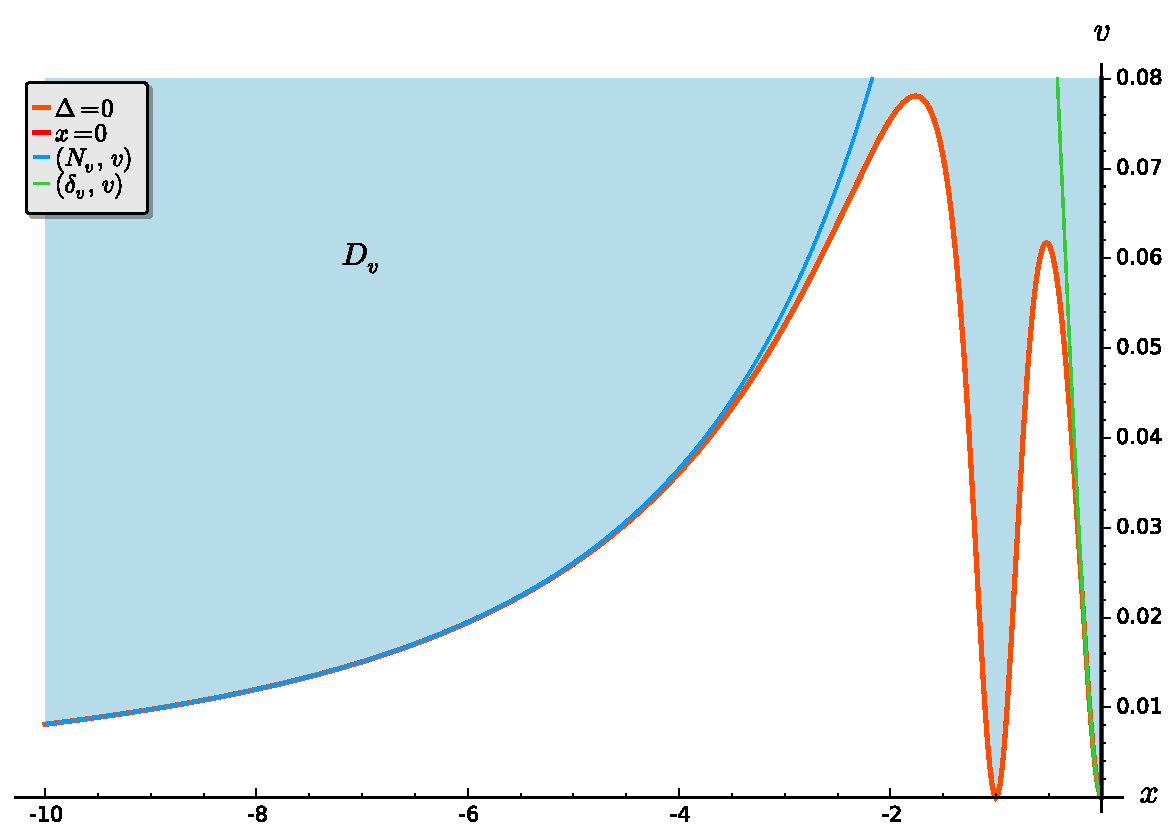
\includegraphics[width=\textwidth]{plots/ch1_15_nice_plot.pdf}};
%\foreach \xx in {0,1,2,...,9}{
%\draw[dashed] ($(img.north west)!0.\xx!(img.north east)$)node[above]{0.\xx} --  ($(img.south west)!0.\xx!(img.south east)$);
%\draw[dashed] ($(img.south east)!0.\xx!(img.north east)$)node[right]{0.\xx} --  ($(img.south west)!0.\xx!(img.north west)$);
%}
%\path ($(img.north west)!0.1!(img.north east)$)|-coordinate(c1)($(img.south east)!0.3!(img.north east)$);% c1: first corner
%\path ($(img.north west)!0.82!(img.north east)$)|-coordinate(c2)($(img.south east)!0.77!(img.north east)$);   %c2 : second corner
%\draw[red,ultra thick,rounded corners] (c1)         rectangle (c2);
%\draw (c1) node {\huge{$\mathscr{A}$}};
%\draw (c2) node[below] {\huge{$\mathscr{B}$}};
%\end{tikzpicture}
%\caption{M1} \label{fig:M1}
%\end{figure}
%--------------------------------------------------------------------%

\end{section}
\end{chapter}

\begin{chapter}{A topological proof for the open quadrant $\Qu$ problem}
\begin{section}{A topological perspective}
%Modificad cualquier cosa que no os convenza o que no sea totalmente cierta de esta introduccion:
Although Fernando, Gamboa and Ueno proved that the open quadrant $\Qu$ is the image of $\R^2$ under two distinct polynomial maps using very different techniques, they developed quite recently in \cite{fgu} a completely new proof that relies on algebraic topology methods applied to a new polynomial map $\FFF: \R^2 \longrightarrow \R^2$. The genesis of this third proof appears in Ueno's Ph.D. \cite{u} written under the supervision of Fernando. 

In this chapter we will build up the topological machinery necessary to prove theorem \ref{openQuad} in a very geometrical way, and completely avoiding the aid of computer calculations.
\begin{subsection}{The new polynomial map}
Without further ado, the polynomial map we are going to work with is denoted $\FFF$ and it is defined as:
\begin{equation*}
\boxed{
\FFF({\tt x}, {\tt y}) := \big(({\tt x}^2{\tt y}^4+{\tt x}^4{\tt y}^2-{\tt y}^2-1)^2+{\tt x}^6{\tt y}^4,\ ({\tt x}^6{\tt y}^2+{\tt x}^2{\tt y}^2-{\tt x}^2-1)^2+{\tt x}^6{\tt y}^4\big).
}
\end{equation*}

As we announced before, in Section \ref{TTT} we will introduce some definitions and prove some facts about a family of topological subspaces of $\R^3$ homeomorphic to a closed disc, and paths that go through them.

\vspace{1mm}

Afterwards, after factorizing $\FFF=f_2\circ f_1$ with $f_2=h\circ g$, it will be clear that the proof is reduced to check that the boundaries of two certain topological subspaces of $\R^3$ homeomorphic to a closed disc meet $g(\overline{\Qu})$, where $\overline{\Qu}:=\set{x\ge 0,y\ge 0}$ is the closed quadrant.
\end{subsection}
\end{section}
\begin{section}{Topological tools}\label{TTT}
\begin{subsection}{Some definitions}\label{topDefs}
We begin by defining the key topological manifolds we are going to work with.
\begin{definitions}
(i) Let ${\mathbb D}_A:=\set{(x,y):x^2+y^2\le A^2}\subset\R^2$ be the closed disc of center the origin and radius $A>0$. A \textit{warped disc} is a subset 
$$
\D_{A,\xi}:=\set{(x,y,z):x^2+y^2\le A^2,\ z=\xi(x,y)}\subset\R^3$$
where $\xi:\R^2\longrightarrow\R$ is a continuous function. Let $\zeta$ be the homeomorphism
$$
\zeta:\R^3\longrightarrow\R^3,\ (x,y,z)\longmapsto\big(x,\, y,\, z-\xi(x,y)\big).
$$
Clearly $\zeta(\D_{A,\xi})={\mathbb D}_A\times\{0\}$ is the projection or ``flattening'' of the warped disc $\D_{A,\xi}$ onto the plane $\{z=0\}\subset\R^3$. We will also call a warped disc the image of $\D_{A,\xi}$ under a permutation of the variables of $\R^3$; namely
\begin{equation*}
\begin{aligned}
\D_{A,\xi}:=\set{(x,y,z): y^2+z^2\le A^2,\ x=\xi(y,z)}& \ \text{ or } \\
\D_{A,\xi}:=\set{(x,y,z): x^2+z^2\le A^2,\ y=\xi(x,z)}&,
\end{aligned}
\end{equation*}
with $\xi$ defined as above.

\vspace{1mm}

(ii) For each $\eps>0$ let us define the following  open neighbourhood of ${\mathbb D}_A$: 
$$
{\mathbb D}_A(\eps):=\set{(x,y):x^2+y^2<(A+\eps)^2}\times(-\eps,\eps)\subset\R^3.
$$ 
As $\zeta$ is a homeomorphism, $\D_{A,\xi}(\eps):=\zeta^{-1}\big({\mathbb D}_A(\eps)\big)\subset\R^3$ is an open neighbourhood of the warped disc $\D_{A,\xi}$. 
\end{definitions}

Next, we recall the notions of \emph{path} and \emph{path concatenation}. Also, we will recall the concept of  \emph{fundamental group} of a (path connected) topological space.

\vspace{1mm}

\begin{definitions}\label{pathDefs}
(i) Let $X$ be a topological space. A continuous map $\alpha:[a,b]\to X$, where $[a,b]\subset\R$ is a closed interval is a \emph{path} in $X$. If $\alpha(a)=\alpha(b)=x_0\in X$, we say that $\alpha$ is a \emph{loop} with base point $x_0$. In such a case, $\alpha$ may be viewed as a map whose domain is the quotient space $[a,b]/\!\sim$ obtained by identifying the end points of $[a,b]$. Notice that $[a,b]/\!\sim$ is homeomorphic to the circumference $\mathbb{S}^1:=\set{(x,y):x^2+y^2=1}\subset\R^2$. After a linear change of variables we may assume, if necessary, that $[a,b]=[0,1]$.

\vspace{1mm}

(ii) Given two paths $\alpha:[0,1]\to X$ and $\beta:[0,1]\to X$ such that  $\alpha(1)=\beta(0)$ the \em concatenation \em (also called \em product \em) of $\alpha$ and $\beta$ is defined as follows:
$$
\alpha*\beta:[0,1]\longrightarrow X,\ t\longmapsto
\left\{\begin{array}{ll}
\alpha(2t) &\text{ if } 0\leq t\leq\tfrac{1}{2},\\
\beta(2t-1) &\text{ if } \tfrac{1}{2}\leq t\leq1.
\end{array}
\right.
$$
The idea under this definition is clear. We use $\alpha$ in the "first part of the path", but the speed must be double of the original one to reach the point $\alpha(1)$ at $t:=\tfrac{1}{2}$. This explains the definition of the first part of the new path. We must use $\beta$ for the second part. Necessarily $(\alpha*\beta)\big(\tfrac{1}{2}\big)=\beta(0)$ and $(\alpha*\beta)(1)=\beta(1)$. To do that, we use the line that joints the points $p:=\big(\tfrac{1}{2},0\big)$ and $q:=(1,1)$, that is $\gamma(t):=2t-1$. Of course this is not at all the only way to construct a path joining $p$ and $q$, but seems to be the simplest one.

It is easily checked that the concatenation of loops enjoys the associative property. Besides, fixed $x_0\in X$, the constant loop $e_{x_0}:[0,1]\to X,\, t\mapsto x_0$ satisfies the equality $e_{x_0}*\alpha=\alpha=\alpha*e_{x_0}$ for every loop $\alpha$ in $X$ of basis $x_0$. In addition, given a loop $\alpha$ in $X$ the loop $\alpha^{-1}:[0,1]\to X, \, t\mapsto\alpha(1-t)$ that travels the same curve as $\alpha$ but in the opposite direction satisfies $\alpha*\alpha^{-1}=\alpha^{-1}*\alpha=e_{x_0}$.

\vspace{1mm}

(iii) Let $I:=[0,1]\subset\R$ and let $X,Y$ be two path-connected topological spaces. A \emph{homotopy} is a continuous map $H: X\times I\longrightarrow Y$. We associate to $H$ the family of continuous maps $\{H_s:X\to Y,\ x\mapsto H(x,s)\}_{s\in I}$, and it is said that the maps $H_0:X\to Y$ and $g:=H_1:X\to Y$ are \em homotopic. \em We denote this with $f\overset{H}{\simeq}g$. If, in addition, $g$ is constant we say that $f$ is \emph{null-homotopic}.

\vspace{1mm} 

(iv) Given a path-connected topological space $X$ and a point $x_0\in X$ we define the \emph{fundamental group of $X$ at the base point $x_0$} as the quotient space of loops of base $x_0$ modulo the ``homotopy relation'', and we denote it with $\pi_1(X,x_0)$. If $\alpha$ is a loop with base point $x_0$, then it represents an element of $\pi_1(X,x_0)$ denoted with $[\alpha]$. The concatenation of loops is compatible with the homotopy relation and endows $\pi_1(X,x_0)$ with an structure of group.

\vspace{1mm}

(v) We impose $X$ to be path connected to be sure that the fundamental groups $\pi_1(X,x_0)$ and $\pi_1(X,x_1)$ corresponding to two distinct points $x_0$ and $x_1$ in $X$ are isomorphic. Indeed, if $\gamma$ is a path in $X$ that connects $x_0$ and $x_1$ we associate to each loop $\alpha$ with base $x_0$ the loop of base $x_1$ defined as the product $\gamma\cdot\alpha\cdot\gamma^{-1}$. This construction is compatible with the homotopy relation, so it induces a homomorphism $\pi_1(X,x_0)\to\pi_1(X,x_1)$. This is in fact an isomorphism because we can associate to every loop $\beta$ with base $x_1$ the loop of base $x_0$ defined as the product $\gamma^{-1}\cdot\beta\cdot\gamma$. This is why it is usual to denote $\pi_1(X)$ the fundamental group of $X$ without any reference to the base point $x_0$. 
\end{definitions}

\vspace{1mm}

(vi) A path connected space $X$ is said to be \em simply connected \em if its fundamental group is trivial, that is, all loops are null-homotopic. Intuitively this means that all loops in $X$ are contractible to a point.

\vspace{1mm}

Next we explain the meaning of \emph{meeting transversally once a warped disc}, which is just a formalization of our intuition.

\begin{definitions} \label{pathDefs1}

(i) A path $\alpha:[a,b]\to\R^3$\emph{meets transversally once the warped disc $\D_{A,\xi}$} if there exist $s_0\in(a,b)$ and $\eps>0$ such that
$$
J:=\alpha^{-1}(\D_{A,\xi}(\eps))=(s_0-\eps,s_0+\eps)
$$
is an open subinterval of $[a,b]$ and 
$$
(\zeta\circ\alpha)|_J(t)=(0,0,t-s_0),
$$
where obviously $(\zeta\circ\alpha)|_J(t)\subset\mathbb{D}_A(\eps)$ because $\alpha|_J(t)\in\zeta^{-1}\big(\mathbb{D}_A(\eps)\big) = \D_{A,\xi}(\eps)$.

\vspace{1mm}

(ii) Let $C$ be a topological space homeomorphic to a closed disc and let $\phi:C\to\R^3$ be a continuous map. The restriction $\partial\phi:=\phi|_{\partial C}$ is called the \textit{boundary map} of $\phi$. We say that the boundary map $\partial\phi$ \emph{meets transversally once a warped disc} $\D_{A,\xi}\subset\R^3$ if there exists a parameterization $\beta:[a,b]\to\partial C\cong\mathbb{S}^1$ such that the path $\alpha:=\phi\circ\beta:[a,b]\to\R^3$ meets transversally once the warped disc $\D_{A,\xi}$.
\end{definitions}


\begin{remark}\label{remPath}
If the path $\alpha:[a,b]\to\R^3$ meets transversally once the warped disc $\D_{A,\xi}$, then $\alpha\big([a,b]\big)\cap\partial\D_{A,\xi}=\varnothing$. This will be helpful in the proof of Proposition \ref{propTop}.
\end{remark}
\end{subsection}

\begin{subsection}{Auxiliary results}
We proceed now to prove some facts that will be helpful later on to prove Theorem \ref{openQuad}. Firstly, we prove in Lemma \ref{lemmaFundGr} that if a loop meets transversaly once a warped disc, then the topological space $\R^3$ minus the border of the warped disc has $\Z$ as fundamental group. Figure \ref{fig:disc} helps to visualize the idea of the proof.

\begin{lemma}\label{lemmaFundGr} \em Let $\D_{A,\xi}\subset\R^3$ be a warped disc and let $X:=\R^3\setminus\partial\D_{A,\xi}$. Let $\alpha:[a,b]\to X$ be a loop with base point $x_0\in X$ that meets transversally once $\D_{A,\xi}$. Then $[\alpha]$ is a generator of $\pi_1(X,x_0)\cong{\mathbb Z}$. \em 
\begin{Proof} 
Using the notation introduced in Definitions \ref{pathDefs} and \ref{pathDefs1}, let $s_0\in(a,b)$ and $\eps>0$ be such that 
$$
J:=\alpha^{-1}\big(\D_{A,\xi}(\eps)\big)=(s_0-\eps,s_0+\eps)\subset[a,b]
$$ 
and $(\zeta\circ\alpha)|_J(t)=(0,0,t-s_0)$. We can assume $s_0=0$ after a reparameterization of $\alpha$; so $J=(-\eps,\eps)$ and $(\zeta\circ\alpha)|_J(t)=(0,0,t)$. Note that we can write the interval $[a,b]$ as $[a,-\eps]\cup(-\eps,\eps)\cup[\eps,b]$.

\vspace{1mm}

Since $\zeta$ is a homeomorphism of $\R^3$, instead of working in the warped disc we will prove the statement for ${\mathbb D}_A$ where $\beta:=\zeta\circ\alpha$, $Y:=\R^3\setminus\partial{\mathbb D}_A$ and the new base point is $y_0:=\beta(-\eps)=(0,0,-\eps)$. Consider the path $\gamma:[0,1]\to\R^3$ (see Figure \ref{fig:disc}) defined in the following way:
$$
\gamma(t):=
\begin{cases}
\big(3(A+\eps)t,\,0,\,\eps\big)&\text{if $0\le t\le\frac{1}{3}$,}\\
\big(A+\eps,\, 0,\, \eps-\big(t-\frac{1}{3}\big)6\eps\big)&\text{if $\frac{1}{3}<t\le \frac{2}{3}$,}\\
\big(A+\eps-3(A+\eps)\big(t-\frac{2}{3}\big),\, 0,\, -\eps\big)&\text{if $\frac{2}{3}<t\le 1$}.
\end{cases}
$$
Let $\beta_0:=\beta|_{J}=\beta|_{(-\eps,\eps)}$ and $\beta_1:=\beta|_{[\eps,b]}\ast\beta|_{[a,-\eps]}$. Using the properties of path concatenation we get:
$$
\quad[\beta]=[\beta_0\ast\beta_1]=\big[\beta_0\ast\big(\gamma\ast\gamma^{-1}\big)\ast\beta_1\big]=[\beta_0\ast\gamma]\,\cdot\,[\gamma^{-1}\ast\beta_1].
$$
We claim that $[\beta_0\ast\gamma]=g$ and $[\gamma^{-1}\ast\beta_1]=e$, where $g$ and $e$ are, respectively, a generator of $\pi_1(Y,y_0)\cong{\mathbb Z}$ and the identity element.

\begin{figure}[ht!]
\begin{center}
\begin{tikzpicture}[scale=0.8,line join=round,decoration={
    markings,
    mark=at position 0.5 with {\arrow[black!80,opacity=0.6]{>}}}]
\tikzstyle{estiloejes} = [line width=1pt]
\tikzstyle{estilodiscos} = [shading=radial]
\tikzstyle{estiloborde1} = [line width=2pt, draw=gray!70, rounded corners=8pt]
\tikzstyle{estiloborde2} = [line width=2pt, decorate]
%Mio
\tikzstyle{estiloborde3} = [line width=2pt, draw=red!70, rounded corners=8pt]
\tikzstyle{estiloborde4} = [line width=2pt, draw=black!50!blue, rounded corners=8pt]
\tikzstyle{estiloborde5} = [line width=2pt, draw=blue!70, rounded corners=8pt]
%------
\tikzstyle{estiloborde} = [line width=2pt]
\draw[estiloejes](-1.164,1.416)--(-1.947,2.368);
\filldraw[fill=gray!50,fill opacity=0.4,draw=none](-.677,.688)--(-.677,2.214)--(-.203,2.248)--(-.203,.722)--cycle;
\filldraw[fill=gray!50,fill opacity=0.4,draw=none](-.203,.722)--(-.203,2.248)--(.277,2.245)--(.277,.719)--cycle;
\draw[estiloejes](0,-3.816)--(0,3.8);
\filldraw[fill=gray!50,fill opacity=0.4,draw=black, dashed](-2.839,-1.316)--(-2.982,-1.093)--(-3.051,-.862)--(-3.045,-.628)--(-2.964,-.398)--(-2.81,-.177)--(-2.587,.03)--(-2.301,.217)--(-1.957,.38)--(-1.566,.515)--(-1.136,.618)--(-.677,.688)--(-.203,.722)--(.277,.719)--(.75,.679)--(1.204,.605)--(1.629,.496)--(2.014,.356)--(2.349,.189)--(2.626,-.001)--(2.839,-.211)--(2.982,-.433)--(3.051,-.665)--(3.045,-.898)--(2.964,-1.128)--(2.81,-1.349)--(2.587,-1.556)--(2.301,-1.743)--(1.957,-1.906)--(1.566,-2.041)--(1.136,-2.145)--(.677,-2.214)--(.203,-2.248)--(-.277,-2.245)--(-.75,-2.206)--(-1.204,-2.131)--(-1.629,-2.022)--(-2.014,-1.883)--(-2.349,-1.716)--(-2.626,-1.525)--cycle;
\filldraw[fill=gray!50,fill opacity=0.4,draw=none](.277,.719)--(.277,2.245)--(.75,2.206)--(.75,.679)--cycle;
\filldraw[fill=gray!50,fill opacity=0.4,draw=none](-1.136,.618)--(-1.136,2.145)--(-.677,2.214)--(-.677,.688)--cycle;
\filldraw[fill=gray!50,fill opacity=0.4,draw=none](.75,.679)--(.75,2.206)--(1.204,2.131)--(1.204,.605)--cycle;
\draw[estiloejes](-1.136,1.382)--(-1.164,1.416);
\filldraw[fill=gray!50,fill opacity=0.4,draw=none](-1.566,.515)--(-1.566,2.041)--(-1.136,2.145)--(-1.136,.618)--cycle;
\filldraw[fill=gray!50,fill opacity=0.4,draw=none](1.204,.605)--(1.204,2.131)--(1.629,2.022)--(1.629,.496)--cycle;
\filldraw[fill=gray!50,fill opacity=0.4,draw=none](-1.957,.38)--(-1.957,1.906)--(-1.566,2.041)--(-1.566,.515)--cycle;
\filldraw[fill=gray!50,fill opacity=0.4,draw=none](1.629,.496)--(1.629,2.022)--(2.014,1.883)--(2.014,.356)--cycle;
\draw[estiloejes](1.136,-1.382)--(-1.136,1.382);
\filldraw[fill=gray!50,fill opacity=0.4,draw=none](-2.301,.217)--(-2.301,1.743)--(-1.957,1.906)--(-1.957,.38)--cycle;
\filldraw[fill=gray!50,fill opacity=0.4,draw=none](2.014,.356)--(2.014,1.883)--(2.349,1.716)--(2.349,.189)--cycle;
\filldraw[fill=gray!50,fill opacity=0.4,draw=none](-2.587,.03)--(-2.587,1.556)--(-2.301,1.743)--(-2.301,.217)--cycle;
\filldraw[fill=gray!50,fill opacity=0.4,draw=none](2.349,.189)--(2.349,1.716)--(2.626,1.525)--(2.626,-.001)--cycle;
\filldraw[fill=gray!50,fill opacity=0.4,draw=none](-2.81,-.177)--(-2.81,1.349)--(-2.587,1.556)--(-2.587,.03)--cycle;
\filldraw[fill=gray!50,fill opacity=0.4,draw=none](2.626,-.001)--(2.626,1.525)--(2.839,1.316)--(2.839,-.211)--cycle;
\filldraw[fill=gray!50,fill opacity=0.4,draw=none](-3.045,-.628)--(-3.045,.898)--(-2.964,1.128)--(-2.964,-.398)--cycle;
\filldraw[fill=gray!50,fill opacity=0.4,draw=none](-3.051,-.862)--(-3.051,.665)--(-3.045,.898)--(-3.045,-.628)--cycle;
\draw[estiloejes](2.839,.553)--(-2.839,-.553);
\draw[estiloejes](0,-.763)--(0,.038);
\filldraw[fill=gray!50,fill opacity=0.4,draw=black,dashed](-2.626,.001)--(-2.349,-.189)--(-2.014,-.356)--(-1.629,-.496)--(-1.204,-.605)--(-.75,-.679)--(-.277,-.719)--(.203,-.722)--(.677,-.688)--(1.136,-.618)--(1.566,-.515)--(1.957,-.38)--(2.301,-.217)--(2.587,-.03)--(2.81,.177)--(2.964,.398)--(3.045,.628)--(3.051,.862)--(2.982,1.093)--(2.839,1.316)--(2.626,1.525)--(2.349,1.716)--(2.014,1.883)--(1.629,2.022)--(1.204,2.131)--(.75,2.206)--(.277,2.245)--(-.203,2.248)--(-.677,2.214)--(-1.136,2.145)--(-1.566,2.041)--(-1.957,1.906)--(-2.301,1.743)--(-2.587,1.556)--(-2.81,1.349)--(-2.964,1.128)--(-3.045,.898)--(-3.051,.665)--(-2.982,.433)--(-2.839,.211)--cycle;
\draw[estiloborde5,decorate,decoration={
    markings,
    mark=at position 0.5 with {\arrow[blue!60,opacity=0.6]{>}}}](-2.839,-.514)--(-2.839,-1.316)--(-.081,-.779);
\draw[estiloborde,draw=blue!60](-2.839,-.514)--(-2.839,-1.316)--(-.081,-.779);
%beta_1 (clarito):
\draw[estiloborde3, opacity=1](-3.9,-.789)--(-3.893,-1.521)--(-3.731,-2.253)--(-3.244,-2.921)--(-2.433,-2.763)--(-1.622,-3.368)--(-.811,-3.211)--(0,-3.053)--(0,-1.526)--(0,-.763)--(0,.238)--(0,.763)--(0,1.526)--(-.811,2.132)--(-2.433,1.816)--(-3.244,2.421)--(-4.056,1.5)--(-4.056,.737)--cycle;
%Mi beta_0 (clarito):
\draw[estiloborde,draw=black!20!blue,opacity=1](-0,0)--(-0,-0.8);
%Disco naranja:
\filldraw[fill opacity=0.5,orange!90,line width=1pt,estilodiscos](-.973,1.222)--(-1.342,1.134)--(-1.678,1.018)--(-1.972,.878)--(-2.218,.718)--(-2.409,.541)--(-2.541,.351)--(-2.61,.154)--(-2.615,-.046)--(-2.556,-.244)--(-2.433,-.436)--(-2.251,-.615)--(-2.013,-.778)--(-1.726,-.922)--(-1.396,-1.041)--(-1.032,-1.134)--(-.643,-1.198)--(-.237,-1.232)--(.174,-1.234)--(.581,-1.206)--(.973,-1.146)--(1.342,-1.057)--(1.678,-.942)--(1.972,-.802)--(2.218,-.641)--(2.409,-.464)--(2.541,-.275)--(2.61,-.077)--(2.615,.123)--(2.556,.321)--(2.433,.512)--(2.251,.691)--(2.013,.855)--(1.726,.998)--(1.396,1.117)--(1.032,1.21)--(.643,1.275)--(.237,1.308)--(-.174,1.311)--(-.581,1.282)--cycle;
\draw[estiloejes,->](0,0)--(0,3.8);
%Mi beta_0 (oscuro):
\draw[estiloborde,draw=black!30!blue,opacity=0.9](-0,1.1)--(-0,0.01);
%beta_1 (oscuro):
\draw[estiloborde3,opacity=0.9](-3.9,-.789)--(-3.893,-1.521)--(-3.731,-2.253)--(-3.244,-2.921)--(-2.433,-2.763)--(-1.622,-3.368)--(-.811,-3.211)--(0,-3.053)--(0,-1.526)(0,.77)--(0,.663)--(0,1.526)--(-.811,2.132)--(-2.433,1.816)--(-3.244,2.421)--(-4.056,1.5)--(-4.056,.737);
\draw[estiloborde3,decorate,decoration={
    markings,
    mark=at position 0.5 with {\arrow[red!80,opacity=0.7]{>}}}]
(-3.98,1.)--(-4.056,-0.5);
\draw[estiloborde3,decorate,decoration={
    markings,
    mark=at position 0.5 with {\arrow[red!80,opacity=0.7]{>}}}]
(-1.622,-3.368)--(-.811,-3.211);
%Mi flecha
\draw[estiloborde4,decorate,decoration={
    markings,
    mark=at position 0.5 with {\arrow[black!30!blue,opacity=0.65]{>}}}]
(0,-0.5)--(0,1.25);
\filldraw[fill=gray!50,fill opacity=0.4,draw=none](-2.964,-.398)--(-2.964,1.128)--(-2.81,1.349)--(-2.81,-.177)--cycle;
\draw[estiloejes](3.319,.646)--(2.911,.567);
\draw[estiloejes](2.911,.567)--(2.839,.553);
\filldraw[fill=gray!50,fill opacity=0.4,draw=none](2.839,-.211)--(2.839,1.316)--(2.982,1.093)--(2.982,-.433)--cycle;
\filldraw[fill=gray!50,fill opacity=0.4,draw=none](2.982,-.433)--(2.982,1.093)--(3.051,.862)--(3.051,-.665)--cycle;
\draw[estiloborde,draw=blue!70](-.081,.747)--(-2.839,.211)--(-2.839,-.514);
\draw[estiloborde5,decorate,decoration={
    markings,
    mark=at position 0.5 with {\arrow[blue!60,opacity=0.6]{>}}}](-.081,.747)--(-2.839,.211)--(-2.839,-.514);
\draw[fill=black, draw=none, fill opacity=0.5] (0,.747) circle (0.1cm);
\draw[fill=black, draw=none, fill opacity=0.3] (0,-.77) circle (0.1cm);
\draw[estiloejes](4.867,.947)--(3.319,.646);
\filldraw[fill=gray!50,fill opacity=0.4,draw=none](3.051,-.665)--(3.051,.862)--(3.045,.628)--(3.045,-.898)--cycle;
\filldraw[fill=gray!50,fill opacity=0.4,draw=none](-2.982,-1.093)--(-2.982,.433)--(-3.051,.665)--(-3.051,-.862)--cycle;
\filldraw[fill=gray!50,fill opacity=0.4,draw=none](3.045,-.898)--(3.045,.628)--(2.964,.398)--(2.964,-1.128)--cycle;
\filldraw[fill=gray!50,fill opacity=0.4,draw=none](-2.839,-1.316)--(-2.839,.211)--(-2.982,.433)--(-2.982,-1.093)--cycle;
\filldraw[fill=gray!50,fill opacity=0.4,draw=none](2.964,-1.128)--(2.964,.398)--(2.81,.177)--(2.81,-1.349)--cycle;
\filldraw[fill=gray!50,fill opacity=0.4,draw=none](-2.626,-1.525)--(-2.626,.001)--(-2.839,.211)--(-2.839,-1.316)--cycle;
\filldraw[fill=gray!50,fill opacity=0.4,draw=none](2.81,-1.349)--(2.81,.177)--(2.587,-.03)--(2.587,-1.556)--cycle;
\filldraw[fill=gray!50,fill opacity=0.4,draw=none](-2.349,-1.716)--(-2.349,-.189)--(-2.626,.001)--(-2.626,-1.525)--cycle;
\draw[estiloejes](-2.839,-.553)--(-2.911,-.567);
\filldraw[fill=gray!50,fill opacity=0.4,draw=none](2.587,-1.556)--(2.587,-.03)--(2.301,-.217)--(2.301,-1.743)--cycle;
\draw[estiloejes](-2.911,-.567)--(-3.063,-.596);
\draw[estiloejes](-3.063,-.596)--(-3.319,-.646);
\draw[estiloejes,->](-3.319,-.646)--(-4.867,-.947);
\filldraw[fill=gray!50,fill opacity=0.4,draw=none](-2.014,-1.883)--(-2.014,-.356)--(-2.349,-.189)--(-2.349,-1.716)--cycle;
\filldraw[fill=gray!50,fill opacity=0.4,draw=none](2.301,-1.743)--(2.301,-.217)--(1.957,-.38)--(1.957,-1.906)--cycle;
\filldraw[fill=gray!50,fill opacity=0.4,draw=none](-1.629,-2.022)--(-1.629,-.496)--(-2.014,-.356)--(-2.014,-1.883)--cycle;
\filldraw[fill=gray!50,fill opacity=0.4,draw=none](1.957,-1.906)--(1.957,-.38)--(1.566,-.515)--(1.566,-2.041)--cycle;
\filldraw[fill=gray!50,fill opacity=0.4,draw=none](-1.204,-2.131)--(-1.204,-.605)--(-1.629,-.496)--(-1.629,-2.022)--cycle;
\filldraw[fill=gray!50,fill opacity=0.4,draw=none](1.566,-2.041)--(1.566,-.515)--(1.136,-.618)--(1.136,-2.145)--cycle;
\filldraw[fill=gray!50,fill opacity=0.4,draw=none](-.75,-2.206)--(-.75,-.679)--(-1.204,-.605)--(-1.204,-2.131)--cycle;
\filldraw[fill=gray!50,fill opacity=0.4,draw=none](1.136,-2.145)--(1.136,-.618)--(.677,-.688)--(.677,-2.214)--cycle;
\filldraw[fill=gray!50,fill opacity=0.4,draw=none](-.277,-2.245)--(-.277,-.719)--(-.75,-.679)--(-.75,-2.206)--cycle;
\filldraw[fill=gray!50,fill opacity=0.4,draw=none](.677,-2.214)--(.677,-.688)--(.203,-.722)--(.203,-2.248)--cycle;
\filldraw[fill=gray!50,fill opacity=0.4,draw=none](.203,-2.248)--(.203,-.722)--(-.277,-.719)--(-.277,-2.245)--cycle;
\draw[estiloejes](1.164,-1.416)--(1.136,-1.382);
\draw[estiloejes,<-](1.947,-2.368)--(1.164,-1.416);
\path (2.271,-2.763) node[left]{$y$} (-5.5,-1.2) node[above right]{$x$} (0,4.4) node[below]{$z$};\path (1.45,0) node[right]{${\mathbb D}_A$} (-0.1,-1.02) node[right]{$y_0$};
\path (0,0.85) node[right]{$y_1$};
\path [black!50!blue] (0.1,-0.1) node[right]{$\beta_0$};
\path (2.5,1.468) node[above right]{${\mathbb D}_A(\eps)$};
\path [red] (-4.3,-1.5) node[below]{$\beta_1$};
\path [blue!90] (-1.1,1.15) node[below]{$\gamma$};
\end{tikzpicture}
\caption{The loop $\beta=\beta_0\ast\beta_1$ meets transversally once the disk ${\mathbb D}_A$. Here $y_0:=\beta(-\eps)$ and $y_1:=\beta(\eps)$, so the path $\beta_0$ goes from $y_0$ to $y_1$ (in purple), $\gamma$ goes from $y_1$ to $y_0$ (in blue) and $\beta_1$ goes from $y_1$ to $y_0$ (in red).}\label{fig:disc}
\end{center}
\end{figure}
Firstly, the loop $\gamma^{-1}\ast\beta_1$ with base point $y_0$ is contained in $\R^3\setminus{\mathbb D}_A$, which is a simply connected space. Thus the loop $\gamma^{-1}*\beta_1$ is null-homotopic and $[\gamma^{-1}*\beta_1]=e \in \pi_1(Y,y_0)$.

\vspace{1mm}

On the other hand, the class $[\beta_0\ast\gamma]$ generates $\pi_1(Y,y_0)$. Indeed, $Y$ has as deformation retract the set $Z:=\partial{\mathbb D}_A(\eps)\cup I_\eps$ where $\partial{\mathbb D}_A(\eps)$ is the boundary of ${\mathbb D}_A(\eps)$ and we denote $I_\eps:=\set{(0,0,z):-\eps\le z\le\eps}$. Finally, since $Z$ is homeomorphic to the union of a sphere and one of its diameters we deduce from Lemma \ref{lemmaZ} that $[\beta_0\ast\gamma]$ is a generator of $\pi_1(Z,y_0)\cong\pi_1(Y,y_0)\cong{\mathbb Z}$, as required.
\qed 
\end{Proof}
\end{lemma}

\vspace{1mm}

\begin{lemma}\label{lemmaZ} \em Let $S:=\set{(x,y,z):x^2+y^2+z^2=A^2}\subset\R^3$ be the sphere of center the origin and radius $A> 0$, let $D$ be one of its diameters and let $M := S\cup D$. If $x_0\in M$ then $\pi_1(M,x_0)\cong\Z$. \em 

\begin{Proof}
Let $x_0\in S\setminus D$ and let $U := M\setminus\set{x_0}$. Also, let $V$ be an small enough  neighbourhood of $x_0$ homeomorphic to a closed disc such that it does not meet the diameter $D$. It is clear that $M\cong U\cup V$. Consider  the group homomorphism
$$
\varphi:\pi_1(U\cap V,x_0)\to\pi_1(U,x_0)
$$
induced by the inclusion map ${\tt j}: (U\cap V)\hookrightarrow U$. As $V$ is a simply connected space, we deduce from the Theorem of Seifert and Van Kampen \cite[Chapter IV: $\mathsection$4, page 95]{m} that 
$$
\pi_1(M,x_0)=\bigslant{\pi_1(U,x_0)}{\text{im}(\varphi)}.
$$
Next, notice that $U$ is homeomorphic to the union of a closed disc with an arc that joints two points of the disc and that doesn't touch its border. Thus, $U$ has $\mathbb{S}^1$ as deformation retract and $\pi_1(U, x_0)\cong \Z$. In addition, as $U\cap V\cong V\setminus\set{x_0}$ the set $U\cap V$ is homeomorphic to a punctured disc, so $\pi_1(U\cap V, x_0)\cong \pi_1(\mathbb{S}^1,x_0) \cong \Z$, and notice that a generator of this fundamental group is a loop contained  in $S\setminus\set{x_0}\subset U$. As $S\setminus\set{x_0}$ is contractible, $\varphi(\pi_1(U\cap V, x_0))=0$, hence $\pi_1(M, x_0) = \pi_1(U, x_0)$ is generated by the class of a loop $\alpha$ as in Figure \ref{fig:sphereZ}. Consequently, $\pi_1(M, x_0)=\Z$ as required.
\qed
\end{Proof}
\end{lemma}

\begin{figure}[h]
\begin{center}
\begin{tikzpicture}
\draw[dashed] (-5,0) arc (180:0:5cm and 1.25cm);
\draw[dashed] (0,5) arc (90:-90:1.5cm and 5cm);
\draw (-3,4)--(0,0)--(3,-4);
\draw [line width=2pt, draw=blue!65, opacity=0.8,rounded corners=8pt] (-3,4)--(0,0)--(3,-4);
\draw (0,0) circle (5cm);
\shade[ball color=blue!10!white,opacity=0.30] (0,0) circle (5cm);
\draw (-5,0) arc (180:360:5cm and 1.25cm);
\draw (0,5) arc (90:270:1.5cm and 5cm);
\draw [line width=2pt, draw=blue!65, rounded corners=8pt] (-3,4) arc (120:-38:4.65cm and 5.4cm);
\draw[line width=2.5pt,rotate=180,decorate,decoration={
markings,
mark=at position 0.5 with {\arrow[black!30!blue,opacity=0.65]{>}}}]
(-4.2,0)--(-2.3,-4.5);
\draw[line width=2.5pt,rotate=218,decorate,decoration={
markings,
mark=at position 0.5 with {\arrow[black!10!blue,opacity=0.45]{>}}}]
(0,-1)--(0,1.45);
\path (-4.1,-4.1) node[right]{\Large{$S$}};
\path (-2.7,2.2) node[right]{\Large{$D$}};
\path [blue!85] (3,3) node[right]{\Large{$\alpha$}};
\end{tikzpicture}
\caption{The set $M:=S\cup D$ and a generator $\alpha$ of $\pi_1(M,x_0)$ from Lemma \ref{lemmaZ}.}\label{fig:sphereZ}
\end{center}
\end{figure}

\begin{lemma}\label{lemmaId} \em Let $C$ be a topological space homeomorphic to a closed disc and let $z_0\in\partial C$. Let $\phi:C\longrightarrow X$ be a continuous map and consider a parameterization $\beta:[a,b]\to\partial C$ such that $\beta(a)=z_0=\beta(b)$. Then $[\phi\circ\beta]$ is the identity element of $\pi_1\big(X,\phi(z_0)\big)$.\em
\begin{Proof} 
Let $\psi:C\to\{x^2+y^2\leq 1\}$ be a homeomorphism. Let $H$ be the continuous map
$$
H:[0,1]\times[a,b]\to X,\ (\rho,t)\mapsto\big(\phi\circ\psi^{-1}\big)\big(\rho\cdot(\psi\circ\beta)(t)+(1-\rho)\cdot\psi(z_0))\big).
$$
Notice that $H(0,t)=\phi(z_0)$ and that $H(1,t)=\phi\big(\beta(t)\big)$. Thus $H$ is a homotopy map between $\phi\circ\beta$ and the constant path, as required.
\qed
\end{Proof}
\end{lemma}

\begin{proposition}\label{propTop}
Let $C$ be a topological space homeomorphic to a closed disc and let $\phi:C\longrightarrow\R^3$ be a continuous map. If the boundary map $\partial\phi$ of $\phi$ meets transversally once a warped disc $\D\subset\R^3$, then $\partial\D\cap\phi\big(\overset{\circ}{C}\big)\neq\varnothing$.
\begin{Proof}
Suppose instead that $\partial\D\cap\phi\big(\overset{\circ}{C}\big)=\varnothing$. Since $\partial\phi$ meets transversally once $\D$ it follows from Remark \ref{remPath} that the image of $\partial C$ under the map $\phi$ does not intersect $\partial\D$. This alongside our initial asumption gives us that $\phi(C)\subset X:=\R^3\setminus\partial\D$.

\vspace{1mm}

Let $\beta:[a,b]\to\partial C$ be a parameterization such that $\beta(a)=z_0=\beta(b)$ for some point $z_0\in\partial C$ such that $\phi\circ\beta$ meets transversally once $\D$. By Lemma \ref{lemmaId} the class $[\phi\circ\beta]$ is the identity element of $\pi_1\big(X,\phi(z_0)\big)$. However $[\phi\circ\beta]$ generates, by Lemma \ref{lemmaFundGr}, the group $\pi_1\big(X,\phi(z_0)\big)\cong\Z$, which leads to a contradiction. Thus, $\partial\D\cap\phi\big(\overset{\circ}{C}\big)\neq\varnothing$, as desired.
\qed
\end{Proof}
\end{proposition}
\end{subsection}
\end{section}

\begin{section}{The topological proof for the open quadrant problem}

\begin{subsection}{Factorizing $\FFF$}
The authors observed in \cite[Section 3]{fgu} that the map $\FFF$ can be factorized as $\FFF=f_2\circ f_1$, where the polynomial maps $f_1, f_2$ are defined as follows:
\begin{align*}
&f_1:\R^2\longrightarrow\R^2,\quad (x,y)\longmapsto\big(x^2,\,y^2\big),\\
&f_2:\R^2\longrightarrow\R^2,\quad (x,y)\longmapsto\big((xy^2+x^2y-y-1)^2+x^3y^2,\,(x^3y+xy-x-1)^2+x^3y^2\big).
\end{align*}
Since $f_1\big(\R^2\big)=\overline{\Qu}$ it is then clear that we just need to prove that
\begin{equation}
f_2\big(\overline{\Qu}\big)=\Qu.
\end{equation}
Note that both components of $f_2$ are strictly positive on $\overline{\Qu}$ so the inclusion $f_2(\overline{\Qu})\subset\Qu$ holds. We need to prove the converse inclusion:
\begin{equation}\label{mainTop}
\Qu\subset f_2\big(\overline{\Qu}\big).
\end{equation}
Indeed $f_2=h\circ g$, where the continuous semialgebraic maps $g, h$ are defined as:
$$
\arraycolsep=2pt\def\arraystretch{1.2}
\begin{array}{crlcl}
g:&\overline{\Qu}\longrightarrow\R^3,&\ (x,y)&\longmapsto&\big(xy^2+x^2y-y-1,\,x^{3/2}y,\,x^3y+xy-x-1\big),\\
h:&\R^3\longrightarrow\R^2,&\ (x,y,z)&\longmapsto&\big(x^2+y^2,\,y^2+z^2\big).\\
\end{array}
$$
In this way we can reduce the proof to show that for each pair of positive real numbers $(A^2,B^2)\in\Qu$ there exists a point $(x_0,y_0)\in\overline{\Qu}$ such that $(h\circ g)(x_0,y_0)=(A^2,B^2)$. This is equivalent to check that
\begin{equation*}
\boxed{
\forall\, \,  (A^2,B^2)\in\Qu:\ h^{-1}\big(\set[\big]{(A^2,B^2)}\big)\ \bigcap\ g\big(\overline{\Qu}\big)\ne\varnothing.
}
\end{equation*}

Let $\Ss:=g\big(\overline{\Qu}\big)$ and fix values $B\ge A>0$. By the definition of $h$ we know that
\begin{align*}
&h^{-1}\big(\set{(A^2,B^2)}\big)=\set[\big]{(x,y): x^2+y^2=A^2,\,y^2+z^2=B^2}\subset\R^2 \, \, \text{ and}\\
&h^{-1}\big(\set{(B^2,A^2)}\big)=\set[\big]{(x,y): y^2+z^2=A^2,\,x^2+y^2=B^2}\subset\R^2.
\end{align*} 
Both of them are the intersection of two orthogonal cylinders. Besides, these sets contain, respectively, the boundaries of the warped discs
\begin{align}
&\D_1:= \set{(x,y,z): x^2+y^2\le A^2,\,z=\xi_1(x,y)} \, \, \text{ and}\label{d1}\\
&\D_2:= \set{(x,y,z): y^2+z^2\le A^2,\,x=\xi_2(y,z)},\label{d2}
\end{align}
for the continuous and semialgebraic functions
\begin{align}
&\xi_1:\R^2\longrightarrow\R,\ (x,y)\longmapsto\sqrt{B^2-\min\{y^2,B^2\}},\label{xi1}\\
&\xi_2:\R^2\longrightarrow\R,\ (y,z)\longmapsto\sqrt{B^2-\min\{y^2,B^2\}},\label{xi2}
\end{align}
see Figure \ref{fig:homeo}.

%% IMAGEN COMENTADA
\begin{comment}
\begin{figure}[!ht]
\begin{center}
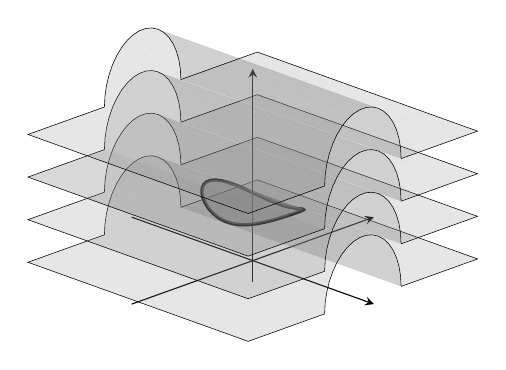
\begin{tikzpicture}
\pgfplotsset{ticks=none}
\begin{axis}[view={45}{30}, scale=1.8, axis lines=middle, footnotesize,xlabel=$$,ylabel=$$,
xmin=-5.5,xmax=5.5,ymin=-9.5,ymax=9.5,zmin=-1,
zmax=9, unit vector ratio=]
\addplot3[opacity=0.0, fill opacity=0.2, surf, gray, samples=5,
variable=\u, variable y=\v,
domain=-5:5, y domain=-9:-3]
({u}, {v}, {0});
\addplot3[opacity=0.0, fill opacity=0.2, surf, gray, samples=5,
variable=\u, variable y=\v,
domain=-5:5, y domain=3:9]
({u}, {v}, {0});
\addplot3[opacity=0.0, fill opacity=0.2, surf, gray, samples=20,
variable=\u, variable y=\v,
domain=-5:5, y domain=0:180]
({u}, {3*cos(v)}, {3*sin(v)});
\addplot3[very thin,mark=,black] plot coordinates {
          (-5,-3,0)
          (-5,-9,0)
          (5,-9,0)
          (5,-3,0)};
\addplot3[very thin,mark=,black] plot coordinates {
          (-5,3,0)
          (-5,9,0)
          (5,9,0)
          (5,3,0)};
\addplot3[very thin,domain=0:pi,samples=20,samples y=0]
({-5},
{3*cos(deg(x))},
{3*sin(deg(x))});
\addplot3[very thin,domain=0:pi,samples=20,samples y=0]
({5},
{3*cos(deg(x))},
{3*sin(deg(x))});
%------
\addplot3[very thick,domain=0:2*pi,samples=40,samples y=0]
({2*cos(deg(x))},
{2*sin(deg(x))},
{sqrt(9-4*(sin(deg(x)))^2)});
\addplot3[opacity=0, fill opacity=0.5, surf,samples=40,gray,
variable=\u, variable y=\v,
domain=0:2, y domain=0:360]
({u*cos(v)},{u*sin(v)},{sqrt(9-u^2*(sin(v))^2)});
%------
\addplot3[opacity=0.0, fill opacity=0.2, surf,gray,samples=5,
variable=\u, variable y=\v,
domain=-5:5, y domain=-9:-3]
({u}, {v}, {2});
\addplot3[opacity=0.0, fill opacity=0.2, surf, gray,samples=5,
variable=\u, variable y=\v,
domain=-5:5, y domain=3:9]
({u}, {v}, {2});
\addplot3[opacity=0.0, fill opacity=0.2, surf, gray, samples=20,
variable=\u, variable y=\v,
domain=-5:5, y domain=0:180]
({u}, {3*cos(v)}, {2+3*sin(v)});
\addplot3[very thin,domain=0:pi,samples=20,samples y=0]
({-5},
{3*cos(deg(x))},
{2+3*sin(deg(x))});
\addplot3[very thin,domain=0:pi,samples=20,samples y=0]
({5},
{3*cos(deg(x))},
{2+3*sin(deg(x))});
\addplot3[very thin,mark=,black] plot coordinates {
          (-5,-3,2)
          (-5,-9,2)
          (5,-9,2)
          (5,-3,2)};
\addplot3[very thin,mark=,black] plot coordinates {
          (-5,3,2)
          (-5,9,2)
          (5,9,2)
          (5,3,2)};
%----
\addplot3[opacity=0.0, fill opacity=0.3, surf,gray,samples=5,
variable=\u, variable y=\v,
domain=-5:5, y domain=-9:-3]
({u}, {v}, {4});
\addplot3[opacity=0.0, fill opacity=0.2, surf, gray,samples=5,
variable=\u, variable y=\v,
domain=-5:5, y domain=3:9]
({u}, {v}, {4});
\addplot3[opacity=0.0, fill opacity=0.2, surf, gray, samples=20,
variable=\u, variable y=\v,
domain=-5:5, y domain=0:180]
({u}, {3*cos(v)}, {4+3*sin(v)});
\addplot3[very thin,domain=0:pi,samples=20,samples y=0]
({-5},
{3*cos(deg(x))},
{4+3*sin(deg(x))});
\addplot3[very thin,domain=0:pi,samples=20,samples y=0]
({5},
{3*cos(deg(x))},
{4+3*sin(deg(x))});
\addplot3[very thin,mark=,black] plot coordinates {
          (-5,-3,4)
          (-5,-9,4)
          (5,-9,4)
          (5,-3,4)};
\addplot3[very thin,mark=,black] plot coordinates {
          (-5,3,4)
          (-5,9,4)
          (5,9,4)
          (5,3,4)};
%----
\addplot3[opacity=0.0, fill opacity=0.2, surf,gray,samples=5,
variable=\u, variable y=\v,
domain=-5:5, y domain=-9:-3]
({u}, {v}, {6});
\addplot3[opacity=0.0, fill opacity=0.2, surf, gray,samples=5,
variable=\u, variable y=\v,
domain=-5:5, y domain=3:9]
({u}, {v}, {6});
\addplot3[opacity=0.0, fill opacity=0.2, surf, gray, samples=20,
variable=\u, variable y=\v,
domain=-5:5, y domain=0:180]
({u}, {3*cos(v)}, {6+3*sin(v)});
\addplot3[very thin,domain=0:pi,samples=20,samples y=0]
({-5},
{3*cos(deg(x))},
{6+3*sin(deg(x))});
\addplot3[very thin,domain=0:pi,samples=20,samples y=0]
({5},
{3*cos(deg(x))},
{6+3*sin(deg(x))});
\addplot3[very thin,mark=,black] plot coordinates {
          (-5,-3,6)
          (-5,-9,6)
          (5,-9,6)
          (5,-3,6)};
\addplot3[very thin,mark=,black] plot coordinates {
          (-5,3,6)
          (-5,9,6)
          (5,9,6)
          (5,3,6)};
%----
\end{axis}
\end{tikzpicture}

\vskip 0.3cm
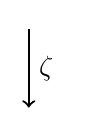
\begin{tikzpicture}
%\draw[white,->] (0,0)--(1,3);
\draw [thick, ->] (0,0)--(0,-0.5) node [right] {$\zeta$} -- (0,-1);
\end{tikzpicture}
\vskip 0.3cm

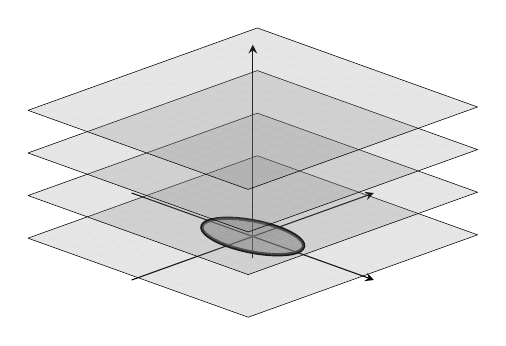
\begin{tikzpicture}
\pgfplotsset{ticks=none}
\begin{axis}[view={45}{30}, scale=1.8, axis lines=middle, footnotesize,xlabel=$$,ylabel=$$,
xmin=-5.5,xmax=5.5,ymin=-9.5,ymax=9.5,zmin=-1,
zmax=9, unit vector ratio=]
\addplot3[opacity=0.0, fill opacity=0.2, surf,gray,samples=20,colormap/hot,
variable=\u, variable y=\v,
domain=-5:5, y domain=-9:9]
({u}, {v}, {0});
\addplot3[very thin,mark=,black] plot coordinates {
          (-5,-9,0)
          (-5,9,0)
          (5,9,0)
          (5,-9,0)
          (-5,-9,0)};
%---
\addplot3[very thick,domain=0:2*pi,samples=40,samples y=0]
({2*cos(deg(x))},
{2*sin(deg(x))},
{0});
\addplot3[opacity=0, fill opacity=0.5, surf,samples=40,gray,
variable=\u, variable y=\v,
domain=0:2, y domain=0:360]
({u*cos(v)},{u*sin(v)},{0});
%---
\addplot3[opacity=0.0, fill opacity=0.2, surf,gray,samples=20,colormap/hot,
variable=\u, variable y=\v,
domain=-5:5, y domain=-9:9]
({u}, {v}, {2});
\addplot3[very thin,mark=,black] plot coordinates {
          (-5,-9,2)
          (-5,9,2)
          (5,9,2)
          (5,-9,2)
          (-5,-9,2)};
\addplot3[opacity=0.0, fill opacity=0.2, surf,gray,samples=20,colormap/hot,
variable=\u, variable y=\v,
domain=-5:5, y domain=-9:9]
({u}, {v}, {4});
\addplot3[very thin,mark=,black] plot coordinates {
          (-5,-9,4)
          (-5,9,4)
          (5,9,4)
          (5,-9,4)
          (-5,-9,4)};
\addplot3[opacity=0.0, fill opacity=0.2, surf,gray,samples=20,colormap/hot,
variable=\u, variable y=\v,
domain=-5:5, y domain=-9:9]
({u}, {v}, {6});
\addplot3[very thin,mark=,black] plot coordinates {
          (-5,-9,6)
          (-5,9,6)
          (5,9,6)
          (5,-9,6)
          (-5,-9,6)};
\end{axis}
\end{tikzpicture}
\caption{The homeomorphism $\zeta$ for $\xi_1(x,y):=\sqrt{B^2-\min(y^2,B^2)}$ acting on $\R^3$. Notice how it ``flattens'' the warped disc $\D_1$.}\label{fig:homeo}
\end{center}
\end{figure}
\end{comment}

Now it is clear that our aim is to prove the following fact:

\begin{center}
\fbox{\textit{For fixed values $B\ge A>0$ the intersections $\partial\D_1\cap\Ss$ and $\partial\D_2\cap\Ss$ are non-empty.}} ($\diamondsuit$)
\end{center}

\end{subsection}

\begin{subsection}{Proof of Claim ($\diamondsuit$)}\label{mainsubsectop}

In order to prove ($\diamondsuit$), we first introduce an auxiliary map $\phi$ and study some of its properties. Let $\phi:=(\phi_1,\phi_2,\phi_3):\R^2\longrightarrow\R^3$, whose components are defined as
$$
\arraycolsep=2pt\def\arraystretch{1.5}
\begin{array}{l}
\phi_1(\rho,\theta)\!:=\!\cos\theta\sin\theta(\cos\theta-
\sin\theta)^2\!+\!\rho(2\cos^4\theta\sin\theta\!+\!\cos\theta\sin^4\theta\!+\!\cos^5\theta)\!+\!\rho^2\cos^5\theta\sin\theta,\\
\phi_2(\rho,\theta)\!:=\!\sqrt{\cos\theta\sin\theta}(\cos\theta+\sin\theta+\rho\cos\theta\sin\theta),\\
\phi_3(\rho,\theta)\!:=\!\rho\sin\theta.
\end{array}
$$

Let also $\Rr:=\big[0,+\infty\big)\times\big(0,\tfrac{\pi}{2}\big)$ and let $\overline{\Rr}:=\big[0,+\infty\big)\times\big[0,\tfrac{\pi}{2}\big]$ be its closure.

\vspace{1mm}

\begin{lemma}\label{phiContainsS}
With the notation introduced above, $\phi(\Rr)\subset\Ss$.
\begin{Proof}
Let $\psi$ be the analytic map
$$
\psi:=(\psi_1,\psi_2):\Rr\to\Qu,\quad(\rho,\theta)\mapsto\left(\frac{\sin\theta}{\cos\theta},\frac{(\cos\theta+\sin\theta+\rho\cos\theta
\sin\theta)\cos^2\theta}{\sin\theta}\right).
$$
Note that $g\circ\psi=\phi|_{\Rr}$. If $\theta\in\big(0,\tfrac{\pi}{2}\big)$ then $\cos\theta,\sin\theta\in(0,1)$, so $\psi$ is well-defined. This together with the fact $\rho\in[0,+\infty)$ implies that $\psi_1,\psi_2$ just attain positive values, so $\psi(\Rr)\subset \Qu\subset \overline{\Qu}$. Thus, $\phi({\Rr})=g(\psi(\Rr))\subset g\big(\overline{\Qu}\big)=\Ss$.
\qed
\end{Proof}
\end{lemma}

\vspace{1mm}

\begin{lemma}\label{phidist}
For all $(\rho,\theta)\in\overline{\Rr}$ the inequality $\phi_1^2(\rho,\theta)+\phi_3^2(\rho,\theta)\ge\frac{\rho^2}{4}$ holds. Thus,
\begin{equation}\label{eq:ineqphi}
\forall (\rho,\theta)\in\overline{\Rr}:\  \text{dist}\big(\phi(\rho,\theta),0\big)\geq\frac{\rho}{2}.
\end{equation}

\begin{Proof}
Notice first that if the inequality $\phi_1^2(\rho,\theta)+\phi_3^2(\rho,\theta)\ge\frac{\rho^2}{4}$ holds, then
$$
\text{dist}\big(\phi(\rho,\theta),0\big)=\sqrt{\phi_1^2(\rho,\theta)+\phi_3^2(\rho,\theta) + \phi_2^2(\rho,\theta)}\ge\sqrt{\frac{\rho^2}{4} + \phi_2^2(\rho,\theta)}\ge\sqrt{\frac{\rho^2}{4}}\ge\frac{\rho}{2},
$$
so \ref{eq:ineqphi} holds. Now, for the first part, if $(\rho,\theta)\in\overline{\Rr}$ then $\cos\theta, \sin\theta \in[0,1]$ and $\rho\ge0$, so we have:
\begin{align*}
\phi_1(\rho,\theta)&\ge\,\rho(\cos\theta\sin^4\theta+\cos^5\theta)=\rho\cos\theta(\cos^4\theta+\sin^4\theta)\\
&=^1\rho\cos\theta(1-2\cos^2\theta\sin^2\theta)=^2\rho\cos\theta\left(1-\frac{\sin^2(2\theta)}{2}\right)
\ge^3 \frac{\rho}{2}\cos\theta.
\end{align*}
In the equality $^1$ we have used that $1^2=(\cos\theta^2+\sin\theta^2)^2=\cos\theta^4+\sin\theta^4+2\cos\theta^2\sin\theta^2$. Equality $^2$ holds because $2\cos\theta\sin\theta=\sin(2\theta)$. Also, as $\theta\in[0,\tfrac{\pi}{2}]$ we have $2\theta\in[0,\pi]$, so $\sin(2\theta)\in[0,1]$. Thus $\sin^2(2\theta)\in[0,1]$ and $\tfrac{\sin(2\theta)}{2}\in[0,\tfrac{1}{2}]$ and inequality $^3$ holds.

\vspace{1mm}

In addition, $\phi_3(\rho,\theta)=\rho\sin\theta\ge\frac{\rho}{2}\sin\theta$, so we obtain the desired inequality:
$$
\phi_1^2(\rho,\theta)+\phi_3^2(\rho,\theta)\ge \frac{\rho^2}{4}\cos^2\theta+\frac{\rho^2}{4}\sin^2\theta=\frac{\rho^2}{4}.
$$
\qed
\end{Proof}
\end{lemma}

\begin{constr}\label{quotConstr}
\em
Recall the elementary equalities
$$
\sin\theta=\cos\Big(\frac{\pi}{2}-\theta\Big)\text{ and } \cos\theta=\sin\Big(\frac{\pi}{2}-\theta\Big)\ \ \forall\theta\in\R.
$$
Thus $\phi(0,\theta)=\phi\big(0,\tfrac{\pi}{2}-\theta\big)$ for $\theta\in[0,\tfrac{\pi}{2}]$. This induces us to make an identification described as follows. Fix $M>0$ and consider the rectangle 
$$
\overline{\Rr}_M:=\big[0,M\big]\times\big[0,\tfrac{\pi}{2}\big]\subset\overline{\Rr}.
$$
Let $\phi_M=\phi|_{\overline{\Rr}_M}$. Now, identify the points $(0,\theta)$ and $(0,\frac{\pi}{2}-\theta)$ for $\theta\in[0,\tfrac{\pi}{2}]$ (see Figure \ref{fig:identify}) and endow the quotient space $\tilde{\overline{\Rr}}_M$ with the quotient topology. Observe that, as a topological manifold with boundary, the interior of $\tilde{\overline{\Rr}}_M$ is the quotient space $\tilde{\Rr}_M$ obtained identifying the points $(0,\theta)$ and $(0,\frac{\pi}{2}-\theta)$ of $\Rr_M:=\big[0,M\big)\times\big(0,\tfrac{\pi}{2}\big)$, where $\theta\in\big(0,\tfrac{\pi}{2}\big)$.

\begin{figure}[!ht]
\begin{center}
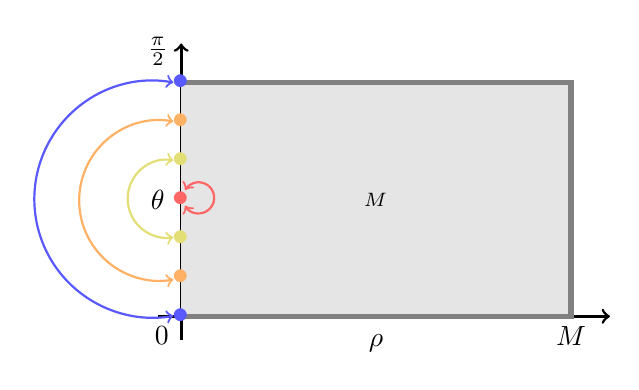
\begin{tikzpicture}[scale=0.99]
\draw[->, line width=1pt] (-0.3,0) -- (5.5,0);
\draw[->, line width=1pt] (0,-0.3) -- (0,3.5);
\draw[gray,line width=2pt,fill=gray!20] (0,3) to (5,3) to (5,0) to (0,0);
\draw (-0.25,-0.25) node{$0$};
\draw (-0.3,1.5) node{$\theta$};
\draw (-0.3,3.4) node{$\tfrac{\pi}{2}$};
\draw (2.5,-0.35) node{$\rho$};
\draw (5,-0.25) node{$M$};
\draw (0,0) node{{\color{blue!65}\large$\bullet$}};
\draw (0,3) node{{\color{blue!65}\large$\bullet$}};
\draw (0,1.5) node{{\color{red!60}\large$\bullet$}};
\draw (0,2.5) node{{\color{orange!60}\large$\bullet$}};
\draw (0,0.5) node{{\color{orange!60}\large$\bullet$}};
\draw (0,2) node{{\color{black!20!yellow!60}\large$\bullet$}};
\draw (0,1) node{{\color{black!20!yellow!60}\large$\bullet$}};
\draw (2.5,1.5) node{$\overline{\Rr}_M$};
\draw [line width=0.8pt, draw=blue!65, <->] (-0.1,3) arc (80:280:1.52cm);
\draw [line width=0.8pt, draw=red!60, <->] (0.05,1.42) arc (210:510:0.2cm);
\draw [line width=0.8pt, draw=orange!60, <->] (-0.1,2.5) arc (80:280:1.03cm);
\draw [line width=0.8pt, draw=black!20!yellow!60, <->] (-0.1,2) arc (80:280:0.5cm);
\end{tikzpicture}
\end{center}
\caption{Idea of the identification in Construction \ref{quotConstr}.}\label{fig:identify}
\end{figure}

Consider the canonical projection $\pi_M:\overline{\Rr}_M\longrightarrow\tilde{\overline{\Rr}}_M$, which is continuous. Since $\phi_M$ is compatible with $\pi_M$, there exists a continuous map $\tilde{\phi}_M:\tilde{\Rr}_M\longrightarrow\R^3$ such that the following diagram is commutative. 

\vspace{1mm}

In addition $\tilde{\phi}_M(\tilde{\Rr}_M)=\phi(\Rr_M)\subset\phi(\Rr)\subset\Ss$ because of Lemma \ref{phiContainsS} and the fact that $\Rr_M\subset\Rr$.
\begin{center}
\begin{tikzpicture}[scale=1.5]
\node (A0) at (0,1) {$\Rr_M$};
\node (A) at (1,1) {$\overline{\Rr}_M$};
\node (C0) at (0,0) {$\tilde{\Rr}_M$};
\node (C) at (1,0) {$\tilde{\overline{\Rr}}_M$};
\node (D) at (2,0) {$\R^3$};

\path[->,font=\scriptsize,>=angle 90]
(A) edge node[above right]{$\phi_M$} (D)
(A) edge node[left]{$\pi_M$} (C)
(A0) edge node[left]{$\pi_M|_{\Rr_M}$} (C0)
(C) edge node[below]{$\tilde{\phi}_M$} (D);

\path[right hook->,font=\scriptsize,>=angle 90]
(A0) edge node[left]{} (A)
(C0) edge node[left]{} (C);

\end{tikzpicture}
\end{center}

\em
\end{constr}

%%%% IMAGEN COMENTADA
\begin{comment}
\begin{figure}[!ht]
\begin{center}
\resizebox{6.2cm}{5cm}{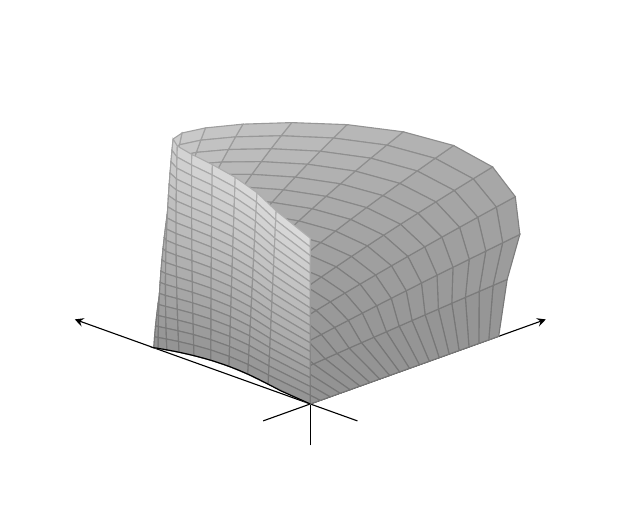
\begin{tikzpicture}%[background rectangle/.style=
%{double,draw=gray},show background rectangle]
\pgfplotsset{ticks=none}
\begin{axis}[point meta min=-4, point meta max=3,view={-45}{30}, scale=2.1, axis lines=middle, footnotesize,xlabel=$$,ylabel=$$,
xmin=-0.5,xmax=2.5,ymin=-0.3,ymax=1.5,zmin=-0.5,zmax=2.5,
unit vector ratio=]
\addplot3[opacity=1, fill opacity=1, surf,samples=20,colormap/blackwhite,
variable=\u, variable y=\v,
domain=0:2, y domain=0:90]
({min(cos(v)*sin(v)*(sin(v)-cos(v))^2+
u*(2*(cos(v))^4*sin(v)+cos(v)*(sin(v))^4+(cos(v))^5)
+u^2*(cos(v))^5*sin(v),10)}, {min(sqrt(sin(v)*cos(v))*(sin(v)+cos(v)
+u*cos(v)*sin(v)),10)}, {min(u*sin(v),10)});
\addplot3[opacity=0.0, fill opacity=0.0,surf,gray,z buffer=sort,samples=40,
variable=\u, variable y=\v,
domain=-1.5:2.5, y domain=0:360]
({3*cos(v)}, {3*sin(v)}, {u});
\addplot3[opacity=1, fill opacity=0.0,domain=0:90,samples=40,samples y=0]
({min(cos(x)*sin(x)*(sin(x)-cos(x))^2,2)}, {min(sqrt(sin(x)*cos(x))*(sin(x)+cos(x)),2)}, {0});
\end{axis}
\end{tikzpicture}}\hskip 0.2cm
\resizebox{6.2cm}{5cm}{
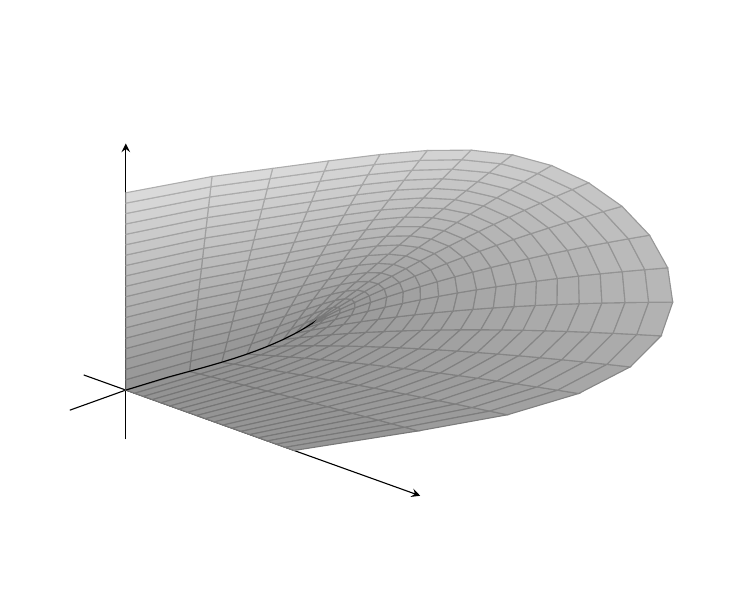
\begin{tikzpicture}
\pgfplotsset{ticks=none}
\begin{axis}[point meta min=-4, point meta max=3,view={45}{30}, scale=2.5, axis lines=middle, footnotesize,xlabel=$$,ylabel=$$,
xmin=-0.5,xmax=3.5,ymin=-0.3,ymax=1.5,zmin=-0.5,zmax=2.5,
unit vector ratio=]
\addplot3[opacity=1, fill opacity=1, surf,samples=20,colormap/blackwhite,
variable=\u, variable y=\v,
domain=0:2, y domain=0:90]
({min(cos(v)*sin(v)*(sin(v)-cos(v))^2+
u*(2*(cos(v))^4*sin(v)+cos(v)*(sin(v))^4+(cos(v))^5)
+u^2*(cos(v))^5*sin(v),10)}, {min(sqrt(sin(v)*cos(v))*(sin(v)+cos(v)
+u*cos(v)*sin(v)),10)}, {min(u*sin(v),10)});
\addplot3[opacity=0.0, fill opacity=0.0,surf,gray,z buffer=sort,samples=40,
variable=\u, variable y=\v,
domain=-1.5:2.5, y domain=0:360]
({3*cos(v)}, {3*sin(v)}, {u});
\addplot3[opacity=1, fill opacity=0.0,domain=0:90,samples=40,samples y=0]
({min(cos(x)*sin(x)*(sin(x)-cos(x))^2,2)}, {min(sqrt(sin(x)*cos(x))*(sin(x)+cos(x)),2)}, {0});
\end{axis}
\end{tikzpicture}%}
}
\caption{Left and right views of $\phi_M(\Rr_M)\subset\Ss$.}\label{pic:surface1}
\end{center}
\end{figure}
\end{comment}

\begin{lemma}\label{RMdisc}
The set $\tilde{\overline{\Rr}}_M$ is homeomorphic to a disc and its boundary is the set
$$
\pi_M\big(\{\rho=M\}\cup\{\theta=0\}\cup\{\theta=\tfrac{\pi}{2}\}\big).
$$
\begin{Proof} Identify $\R^2$ with $\C$ (interchanging the order of the variables $(\rho,\theta)\leadsto(\theta,\rho)$) and consider the continuous map defined as 
$$
\mu:\C\longrightarrow\C,\ z:=\theta+{\tt i}\rho\longmapsto w:=u+{\tt i}v=\big(\tfrac{4}{\pi}z-1\big)^2,
$$
where ${\tt i}$ is the imaginary unit $\sqrt{-1}$. The restriction $\mu|_{\{\rho>0\}}:\{\rho>0\}\to\C\setminus\big([0,+\infty)\times\{0\}\big)$ is a homeomorphism. Now observe that the image of $\overline{\Rr}_M\setminus\{\rho=0\}$ is
$$
\Tt_M:=\big\{(u,v)\in\R^2:\ \big(\tfrac{\pi v}{8M}\big)^2-\big(\tfrac{4M}{\pi}\big)^2\leq u\leq1-\big(\tfrac{v}{2}\big)^2\big\}\setminus\set[\big]{(u,0):u\in[0,1]}.
$$
The closure $\overline{\Tt}_M$ of $\Tt_M$ is a compact convex set because it is a closed bounded intersection of two convex sets, see Figure \ref{fig:Tm}. This implies, by \cite[Corolary 11.3.4]{b}, that $\overline{\Tt}_M$ is homeomorphic to a closed disc. In addition, the map
$$
\mu|_{\set{\rho=0}}:\{\rho=0\}\to\set[\big]{(u,0):u\in[0,+\infty)},\ \theta\mapsto\big(\tfrac{4}{\pi}\theta-1\big)^2
$$
maps the segment $[0,\tfrac{\pi}{2}]\times\set{0}$ onto the interval $[0,1]\times\set{0}$ and the fiber $(\mu|_{\set{\rho=0}})^{-1}(t_0)$ for $t_0\in[0,1]$ consists of two points, namely: 
$$
\set[\big]{\theta_1:=\tfrac{\pi}{4}\big(1+\sqrt{t_0}\big),\, \, \theta_2:=\tfrac{\pi}{4}\big(1-\sqrt{t_0}\big)},
$$
which makes sense considering the identification described in Construction \ref{quotConstr}.

\begin{figure}[!ht]
\begin{center}
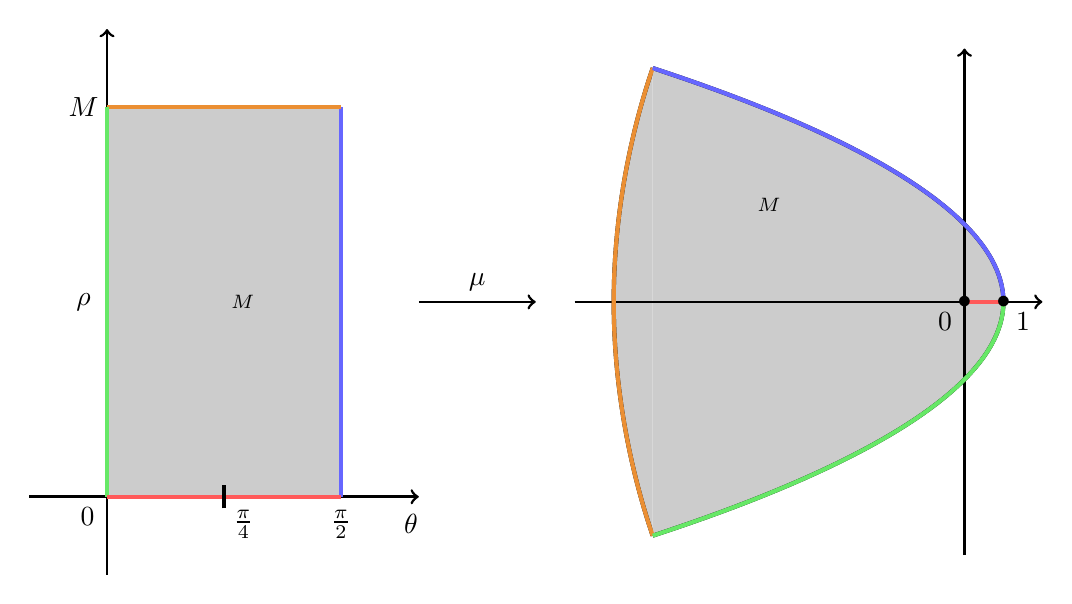
\begin{tikzpicture}[scale=0.99]
%\draw[style=help lines,step=0.5cm] (0,0) grid (12.5,5);
\begin{scope}[scale=0.5,xshift=4cm, yshift=5cm]
%\draw[line width=1.5pt,rotate=-90,draw,fill=gray!40] (6,11) parabola bend (0,20) (-6,11) parabola bend (0,10) (6,11);
%--------------- Mio
\draw[line width=1.5pt,rotate=-90,draw,fill=gray!40] (-6,11) parabola bend (0,10) (6,11);
\draw[line width=1.5pt,rotate=-90,draw,fill=gray!40] (6,11) parabola bend (0,20) (-6,11);
%---------------
\draw[->, line width=1pt] (9,0) -- (21,0);
\draw[->, line width=1pt] (19,-6.5) -- (19,6.5);
%--------------- Mio
\draw[draw=black!10!orange!80,line width=1.5pt,rotate=-90,draw] (-6,11) parabola bend (0,10) (6,11);
\draw[draw=blue!60,line width=1.5pt,rotate=-90,draw] (0,20) parabola bend (0,20) (-6,11);
\draw[draw=black!15!green!60,line width=1.5pt,rotate=-90,draw] (6,11) parabola bend (0,20) (0,20);
%---------------
\draw (20.5,-0.5) node{$1$};
\draw (18.5,-0.5) node{$0$};
\draw (14,2.5) node{$\overline{\Tt}_M$};
\draw[draw=red!65,line width=1.5pt] (19,0) -- (20,0);
\draw (19,0) node{$\bullet$};
\draw (20,0) node{$\bullet$};
\end{scope}
\draw[draw=none, fill=gray!40] (0.5,0) to (3.5,0) to (3.5,5) to (0.5,5) to (0.5,0);
%\draw[draw=blue!60,line width=1.5pt] (3.5,0) to (3.5,5) to (0.5,5) to (0.5,0);
\draw[->, line width=1pt] (-0.5,0) -- (4.5,0);
\draw[->, line width=1pt] (0.5,-1) -- (0.5,6);
%--------------- Mio
\draw[draw=blue!60,line width=1.5pt] (3.5,0) to (3.5,5);
\draw[draw=black!10!orange!80,line width=1.5pt] (3.5,5) to (0.5,5);
\draw[draw=black!15!green!60,line width=1.5pt] (0.5,5) to (0.5,0);
%---------------
\draw[draw=red!65,line width=1.5pt] (0.5,0) to (3.5,0);
\draw[line width=1.5pt] (2,-0.15) -- (2,0.15);
\draw [line width=1pt, ->] (4.5,2.5)--(5.25,2.5) node [above] {$\mu$} -- (6,2.5);
\draw (0.25,-0.25) node{$0$};
\draw (3.5,-0.35) node{$\tfrac{\pi}{2}$};
\draw (4.4,-0.35) node{$\theta$};
\draw (2.25,-0.35) node{$\tfrac{\pi}{4}$};
\draw (0.2,5) node{$M$};
\draw (2.25,2.5) node{$\overline{\Rr}_M$};
\draw (0.2,2.5) node{$\rho$};
\end{tikzpicture}
\end{center}
\caption{Behavior of the map $\mu:\overline{\Rr}_M\longrightarrow\overline{\Tt}_M$.}\label{fig:Tm}
\end{figure}

Following Construction \ref{quotConstr} and since $\theta_1=\tfrac{\pi}{2}-\theta_2$, the map $\lambda:=\mu|_{\overline{\Rr}_M}:\overline{\Rr}_M\to\overline{\Tt}_M$ factors through $\tilde{\overline{\Rr}}_M$ and there exists a continuous map $\tilde{\lambda}:\tilde{\overline{\Rr}}_M\to\overline{\Tt}_M$ such that the following diagram is commutative:
\begin{center}
\begin{tikzpicture}[scale=1.5]
\node (A0) at (0,1) {$\Rr_M$};
\node (A) at (1,1) {$\overline{\Rr}_M$};
\node (C0) at (0,0) {$\tilde{\Rr}_M$};
\node (C) at (1,0) {$\tilde{\overline{\Rr}}_M$};
\node (D) at (2,0) {$\Tt_M$};

\path[->,font=\scriptsize,>=angle 90]
(A) edge node[above right]{$\lambda$} (D)
(A) edge node[left]{$\pi_M$} (C)
(A0) edge node[left]{$\pi_M|_{\Rr_M}$} (C0)
(C) edge node[below]{$\tilde{\lambda}$} (D);

\path[right hook->,font=\scriptsize,>=angle 90]
(A0) edge node[left]{} (A)
(C0) edge node[left]{} (C);
\end{tikzpicture}
\end{center}
The map $\tilde{\lambda}$ is continuous and bijective and in fact it is a homeomorphism because $\tilde{\overline{\Rr}}_M$ is compact and $\overline{\Tt}_M$ is a Hausdorff space. Thus, $\tilde{\overline{\Rr}}_M$ is homeomorphic to a disc and its boundary is 
$$
\pi_M\big(\set{\rho=M}\cup\set{\theta=0}\cup\set{\theta=\tfrac{\pi}{2}}\big),
$$
which concludes the proof.
\qed
\end{Proof}
\end{lemma}

\vspace{1mm}

We are ready to prove  the main result of this section, which will be the key to prove Theorem \ref{openQuad}.

\vspace{1mm}

\begin{lemma}\label{mainlemmatop}
Fix $B\ge A>0$ and consider the warped discs $\D_1$ and $\D_2$ introduced in \eqref{d1} and \eqref{d2}. Then, there exists $M>0$ such that the boundary map $\partial\tilde{\phi}_M:\partial\tilde{\overline{\Rr}}_M\longrightarrow\R^3$ meets transversally once both discs $\D_1$ and $\D_2$.
\begin{Proof} First, since $\D_1$ and $\D_2$ are bounded, there exists $M_0>0$ such that 
$$
\D_1\cup\D_2\subset\set{(x,y,z):\norm{(x,y,z)}<M_0}\subset\R^3.
$$
Take $M:=4M_0$ and consider the set $\tilde{\overline{\Rr}}_M$ and the continuous map $\tilde{\phi}_M$ introduced in Construction \ref{quotConstr}.

\vspace{1mm}

We are going to prove that the boundary map $\partial\tilde{\phi}_M:\partial\tilde{\overline{\Rr}}_M\rightarrow\R^3$ meets transversally once $\D_1$.

\begin{figure}[!ht]
\begin{center}
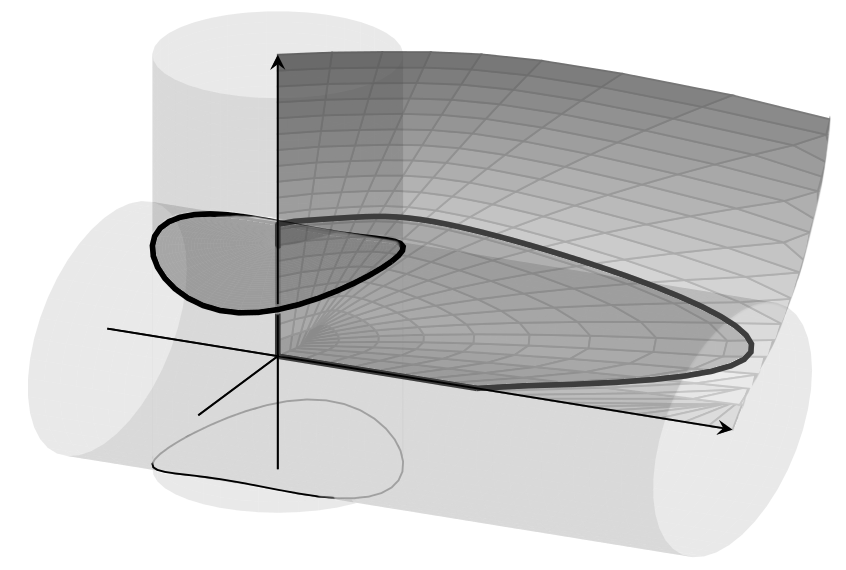
\includegraphics[height=6cm]{plots/ch3_02_B2.png}
\end{center}
\caption{The boundary map $\partial\tilde{\phi}_M:\partial\tilde{\overline{\Rr}}_M\rightarrow\R^3$ meets transversally once $\D_1$.}
\end{figure}

Consider the parameterization of $\partial\tilde{\overline{\Rr}}_M$ given by
$$
\beta_1(t):=
\begin{cases}
\pi_M\big(t,\frac{\pi}{2}\big) &\text{if $0\le t\le M$},\\
\pi_M\big(M,M+\frac{\pi}{2}-t\big) &\text{if $M<t\le M+\frac{\pi}{2}$},\\
\pi_M\big(2M+\frac{\pi}{2}-t,0\big) &\text{if $M+\frac{\pi}{2}<t\le 2M+\frac{\pi}{2}$}.
\end{cases}
$$ 

\begin{figure}[!ht]
\begin{center}
\begin{tikzpicture}[scale=0.99]
\draw[->, line width=1pt] (-0.5,0) -- (5.5,0);
\draw[->, line width=1pt] (0,-0.5) -- (0,3.5);
\draw[draw=blue!60,line width=2pt,fill=gray!20] (0,3) to (5,3) to (5,0) to (0,0);
\draw[draw=blue!60,line width=2pt,->,>=angle 45] (0,3) to (2.75,3);
\draw[draw=blue!60,line width=2pt,->,>=angle 45] (5,3) to (5,1.25);
\draw[draw=blue!60,line width=2pt,->,>=angle 45] (5,0) to (2.25,0);
\draw[->, line width=1pt] (6.5,0) -- (12.5,0);
\draw[->, line width=1pt] (7,-0.5) -- (7,3.5);
\draw[draw=red!65,line width=2pt,fill=gray!20] (7,3) to (12,3) to (12,0) to (7,0);
\draw[draw=red!65,line width=2pt,->,>=angle 45] (12,3) to (9.25,3);
\draw[draw=red!65,line width=2pt,->,>=angle 45] (12,0) to (12,1.75);
\draw[draw=red!65,line width=2pt,->,>=angle 45] (7,0) to (9.75,0);
\draw (-0.25,-0.25) node{$0$};
\draw (-0.3,1.5) node{$\theta$};
\draw (-0.3,3) node{$\tfrac{\pi}{2}$};
\draw (2.5,-0.35) node{$\rho$};
\draw (5,-0.25) node{$M$};
\draw (0,0) node{{\color{blue!60}\large$\bullet$}};
\draw (0,3) node{{\color{blue!60}\large$\bullet$}};
\draw (1.5,1.5) node{identified!};
\draw[->,thick] (1.25,1.75) -- (0.2,2.8);
\draw[->,thick] (1.25,1.25) -- (0.2,0.2);
\draw (2.5,3.5) node{$\beta_1(t)$};
\draw (6.75,-0.25) node{$0$};
\draw (6.7,1.5) node{$\theta$};
\draw (6.7,3) node{$\tfrac{\pi}{2}$};
\draw (9.5,-0.35) node{$\rho$};
\draw (12,-0.25) node{$M$};
\draw (7,0) node{{\color{red!65}\large$\bullet$}};
\draw (7,3) node{{\color{red!65}\large$\bullet$}};
\draw (8.5,1.5) node{identified!};
\draw[->,thick] (8.25,1.75) -- (7.2,2.8);
\draw[->,thick] (8.25,1.25) -- (7.2,0.2);
\draw (9.5,3.5) node{$\beta_2(t)$};
\end{tikzpicture}
\end{center}
\caption{Behavior of the paths $\beta_1$ and $\beta_2$, surrounding $\tilde{\overline{\Rr}}_M$.}\label{fig:betas}
\end{figure}

Let $\alpha_1(t):=\tilde{\phi}_M\circ\beta_1(t)$ defined as:
$$
\alpha_1(t)=\begin{cases}
\phi\big(t,\frac{\pi}{2}\big) &\text{if $0\le t\le M$},\\
\phi\big(M,M+\frac{\pi}{2}-t\big) &\text{if $M<t\le M+\frac{\pi}{2}$},\\
\phi\big(2M+\frac{\pi}{2}-t,0\big) &\text{if $M+\frac{\pi}{2}<t\le 2M+\frac{\pi}{2}$}.
\end{cases}
$$ 

Choose $\eps$ such that $0<\eps<\min\{B,M_0-B\}$ and consider the homeomorphism
$$
\zeta_1:\R^3\to\R^3,\ (x,y,z)\mapsto(x,y,z-\xi_1(x,y)),
$$
where $\xi_1$ is the continuous semialgebraic function introduced in \eqref{xi1}. Let us abbreviate $\D_1(\varepsilon):=\zeta_1^{-1}\big({\mathbb D}_A(\varepsilon)\big)$. As we have done in other proofs we can rely on ${\mathbb D}_A(\varepsilon)$ to conclude this part of the proof, so is enough to check the equality:
$$
\alpha_1^{-1}(\D_1(\varepsilon))=(B-\varepsilon,B+\varepsilon). 
$$

If $t_0\in[0,2M+\frac{\pi}{2}]$, pick $p_0:=\alpha_1(t_0)\in\text{im}(\alpha_1)$. The definition of $\alpha_1$ leads us to distinguish three cases:

\begin{enumerate}[(i)]
\item If $0\le t_0\le M$, then 
$$
\zeta_1(p_0)=\zeta_1(\alpha(t_0))=\zeta_1(\phi(t_0,0))=\zeta_1(\phi(t_0,\tfrac{\pi}{2}))=(0,0,t_0-B),
$$
where $\phi$ was introduced at the beginning of \ref{mainsubsectop}. Thus, $\zeta_1(p_0)\in{\mathbb D}_A(\varepsilon)$ if and only if $-B<-\varepsilon<t_0-B<\varepsilon<M-B$, that is, $0<B-\varepsilon<t_0<B+\varepsilon<M$. 

\item If $M<t_0\le M+\frac{\pi}{2}$ we have by \eqref{eq:ineqphi}, for every point $q\in\D_1(\varepsilon)$,  
$$
\text{dist}(p_0,0)=\text{dist}\big(\phi\big(M,M+\tfrac{\pi}{2}-t\big),0\big)\geq\tfrac{M}{2}=2M_0>\sqrt{2}M_0>\text{dist}(q,0).
$$ 
Therefore $p_0\notin\D_1(\varepsilon)$.

\item If $M+\frac{\pi}{2}<t_0\le 2M+\frac{\pi}{2}$, then 
$$
p_0=\alpha_1(t_0)=\phi\big(2M+\tfrac{\pi}{2}-t_0,0\big)=\big(2M+\tfrac{\pi}{2}-t_0,0,0\big),
$$ 
so $\zeta_1(p_0)=(2M+\tfrac{\pi}{2}-t_0,0,-B)$. As $\varepsilon<B$, we have $\zeta_1(p_0)\not\in{\mathbb D}_A(\varepsilon)$ and $p_0\not\in\D_1(\varepsilon)$.
\end{enumerate}

We conclude $\alpha_1^{-1}\big(\D_1(\varepsilon)\big)=\big(B-\varepsilon,B+\varepsilon\big)$, so $\alpha_1$ meets transversally once $\D_1$. 

Analogously one shows that the boundary map $\partial\tilde{\phi}_M:\partial\tilde{\overline{\Rr}}_M\longrightarrow\R^3$ meets transversally once $\D_2$.

\begin{figure}[!ht]
\begin{center}
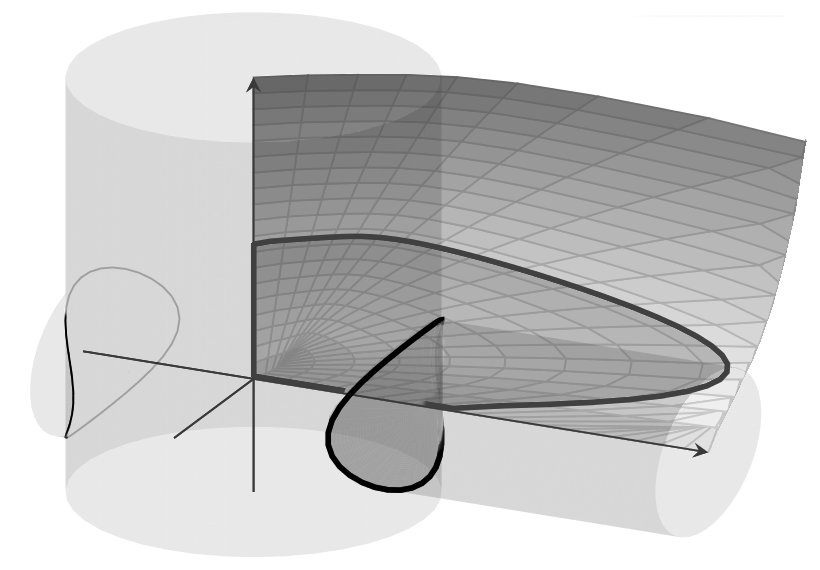
\includegraphics[height=6cm]{plots/ch3_01_A2.png}
\end{center}
\caption{The boundary map $\partial\tilde{\phi}_M:\partial\tilde{\overline{\Rr}}_M\rightarrow\R^3$ meets transversally once $\D_2$.}
\end{figure}

\vspace{1mm}

Consider in this case the parameterization of $\partial\tilde{\overline{\Rr}}_M$ given by
$$
\beta_2(t):=
\begin{cases}
\pi_M\big(t,0\big) &\text{if $0\le t\le M$},\\
\pi_M\big(M,t-M\big) &\text{if $M<t\le M+\frac{\pi}{2}$},\\
\pi_M\big(2M+\frac{\pi}{2}-t,\frac{\pi}{2}\big) &\text{if $M+\frac{\pi}{2}<t\le 2M+\frac{\pi}{2}$},
\end{cases}
$$ 
(see Figure \ref{fig:betas}). Then we define $\alpha_2(t):=\tilde{\phi}_M\circ\beta_2(t)$ as:
$$
\alpha_2(t) =
\begin{cases}
\phi\big(t,0\big) &\text{if $0\le t\le M$},\\
\phi\big(M,t-M\big) &\text{if $M<t\le M+\frac{\pi}{2}$},\\
\phi\big(2M+\frac{\pi}{2}-t,\frac{\pi}{2}\big) &\text{if $M+\frac{\pi}{2}<t\le 2M+\frac{\pi}{2}$}.
\end{cases}
$$ 

Proceed as above keeping the same values for $A$ and $\varepsilon$ and using in this case the homeomorphism
$$
\zeta_2:\R^3\to\R^3,\ (x,y,z)\longmapsto(z,y,x-\xi_2(z,y)),
$$
where $\xi_2$ is the continuous semialgebraic function introduced in \eqref{xi2}, to prove that $\alpha_2$ meets transversally once the warped disk $\D_2$. This concludes the proof.
\qed
\end{Proof}
\end{lemma}

Now we are ready to prove ($\diamondsuit$) and this way conclude the topological proof.

\vspace{2mm}		

[Proof of Theorem \ref{openQuad}] Note first that, by Lemma \ref{RMdisc}, $\overline{\Rr}_M$ is homeomorphic to a closed disc. By Proposition \ref{propTop} applied to the continuous map $\phi_M:\overline{\Rr}_M\to\R^3$ and Lemma \ref{mainlemmatop}, we deduce that the boundaries of both warped discs $\D_1$ and $\D_2$ meet $\phi_M({\Rr}_M)\subset\Ss$. Thus, ($\diamondsuit$) holds, and this concludes the proof.
\qed

\end{subsection}
\end{section}
\end{chapter}


%Pendiente: Añadir consecuencia ---> El interior y el complementario de un ángulo son imágenes polinómicas de R^2 (Tesis Ueno)
\appendix
\begin{chapter}{Auxiliary definitions and results}\label{AA}

\begin{section}{Real algebraic geometry basics}
In this section we give a basic insight into the required concepts, definitions and results from real algebraic geometry. They are mostly used on the first chapter.

We begin with some definitions like \emph{real closed field} and \emph{semialgebraic set}. The \emph{Transfer Principle} allows us to move our results from $\R$ to an arbitrary real closed field $R$. We also give an overview of the \emph{Zariski topology}, in order to talk about concepts like closure or \emph{reducibility} in this topology. Finally, after defining other notions as \emph{proper maps} and \emph{germ Nash half-branch curves}, we finish the section recalling \emph{Puiseux series}, since this is the nature of the solutions of the equation $\Delta_v(x)=0$ in the first proof of Theorem \ref{openQuad}.
\begin{definition}\label{realCField}
	A \em real closed field \em is an ordered field $R$ such that $R(\sqrt{-1})$ is an algebraically closed field. There exist many characterizations of real closed fields. A very enlightening one is the following: $R$ is a real closed field if it is an ordered field that shares with the field $\R$ of real numbers its properties of the first-order language of ordered fields. 
\end{definition}

Indeed, \hyperref[tarskiSeidenberg]{Tarski-Seidenberg Theorem} admits a useful formulation in model theory that explains accurately our last sentence.

\begin{definitions}\label{semialgSet} (i) Let $R$ be a real closed field. A subset $S\subset R^n$ is \em semialgebraic \em if it is defined as a finite union of sets defined by a conjunction of polynomial equalities and inequalities: 
	\begin{equation*}
	\left\{
	\begin{aligned}
		P_1({\tt x}_1,\, .\,&.\,.\,,{\tt x}_n)=0\\
		&\vdots\\
		P_r({\tt x}_1,\, .\,&.\,.\,,{\tt x}_n)=0\\
		Q_1({\tt x}_1,\, .\,&.\,.\,,{\tt x}_n)>0 \\
		&\vdots\\
		Q_{\ell}({\tt x}_1,\, .\,&.\,.\,,{\tt x}_n)>0\\
	\end{aligned}
	\right.
	\end{equation*}
It is easily seen that finite unions and intersections of semialgebraic sets are semialgebraic sets too. In addition, the complementary set of a semialgebraic set is also a semialgebraic set. The easy proof of these facts can be studied in \cite{bcr}, Ch.2.
	
	
(ii) A map $f:S\to T$ between semialgebraic subsets $S\subset R^n$ and $T\subset R^m$ is \em semialgebraic \em if its graph is a semialgebraic subset of $R^{m+n}$.  \end{definitions}


(iii) A \em semialgebraic homeomorphism \em between two semialgebraic subsets $S\subset R^n$ and $T\subset R^m$ is a continuous and bijective semialgebraic map $f:S\to T$. It is easily seen that in such a case its inverse $f^{-1}:T\to S$ is also semialgebraic.

\begin{theorem}[\em Transfer Principle\em]\label{TP} \em Let ${\mathcal L}(R)$ be the first-order language of ordered fields with parameters in the real closed field $R$ and let $\Phi$ be a formula of ${\mathcal L}(R)$. Then, there exists a quantifier-free formula $\Psi$ of ${\mathcal L}(R)$ with the same free variables ${\tt x}_1,\dots,{\tt x}_n$ as $\Phi$ such that, for every real closed field extension $K$ of $R$ and every $x\in K^n$, the sentence $\Phi(x)$ holds true if and only if $\Psi(x)$ holds true.\em

\end{theorem}

\begin{definition}[Zariski topology]\label{zariski} (i) Let $K$ be a field. A subset $X\subset K^n$ is \em algebraic \em if it is the set of common zeros of a finite family of polynomials $f_1,\dots,f_m\in K[{\tt x}_1,\dots,{\tt x}_n]$. 

(ii) The \em Zariski topology \em of an algebraic set $X\subset K^n$ is the topology whose closed sets are the algebraic subsets of $K^n$ contained in $X$. It is indeed a topology, that is, the arbitrary intersection of algebraic sets is also an algebraic set as an straightforward consequence of Hilbert's basis theorem.

(iii) An algebraic subset $X\subset K^n$ is said to be \em reducible \em if there exist algebraic subsets $Y\subsetneq X$ and  $Z\subsetneq X$ such that $X=Y\cup Z$. If $X$ is not reducible it is said to be  \em irreducible. \em 
\end{definition}

\begin{definition}\label{pureDim} (i) Let $S\subset\R^n$ be a semialgebraic set and $p\in S$. The \em local dimension of $S$ at $p$, \em denoted $\dim(S_p)$, is the largest non-negative integer $d$ such that for every open ball $B$ centered at $p$ the intersection $S\cap B$ contains a semialgebraic subset semialgebraically homeomorphic to the cube $[0,1]^d$.

	It is said that $S$ is \em pure dimensional \em if $\dim(S_p)=\dim(S_q)$ for every pair of points $p,q\in S$.
\end{definition}

\begin{definitions}\label{properMap}
	  (i) A continuous map $f:X\to Y$ between topological spaces $X$ and $Y$ is said to be \em proper \em if $f^{-1}(K)$ is a compact subspace of $X$ for every compact subspace $K$ of $Y$. 
	  
	  (ii) A semialgebraic map $f:S\to T$ between semialgebraic sets $S\subset R^n$ and $T\subset R^m$ is said to be \em semialgebraically proper \em if $f^{-1}(K)$ is bounded and closed in $S$ for every bounded and closed in $T$ subset $K$ of $T$.  
\end{definitions}

\begin{definition}\label{dominant}
	A polynomial map $f:X\to Y$ between algebraic sets $X$ and $Y$ is said to be \em dominant \em if its image $f(X)$ is a dense subset of $Y$ in its Zariski topology. 
\end{definition}

\begin{definitions}\label{curveGerms}
	(i) A function $f:U\to\R$ defined in an open semialgebraic subset $U\subset\R^n$ is a \em Nash function \em if it is analytic and semialgebraic. 
	
	(ii) A map $f:=(f_1,\dots,f_m):U\to\R^m$ is a \em Nash map \em if each coordinate $f_i:U\to\R$ is a Nash function. 
	
	(iii) Let $\Gamma\subset\R^n$ be an algebraic curve and $p\in\Gamma$. For every small enough $\eps>0$ the intersection $B_{\eps}\cap\Gamma\setminus\{a\}$, % Aqui no sería p en vez de a?
where $B_{\eps}\subset\R^n$ is the open ball of radius $\eps$ centered at the point $p$, has finitely many connected components $C_1,\dots,C_k$. Each $C_i$ is semialgebraically homeomorphic to the interval $(0,1]$ and in fact for $i=1,\dots,k$ there exists a Nash homeomorphism  $f_i:[0,1]\to C_i\cup\{p\}$, with $f_i(0)=p$.

Indeed, this result is a particular case of the local conic structure theorem of semialgebraic sets, \cite[IX.3.6]{bcr}. 
	
Observe that, by its very definition, it makes sense to define the germs $C_{i,p}$ of $C_i$ at the point $p$ for $i=1,\dots,k$ as they are independent of the radius $\eps$. These germs  $C_{i,p}$ are called the \em germ Nash half-banches \em of the curve $\Gamma$ centered at $p$. For more details see \cite[IX.5.2]{bcr}. 
\end{definitions}

\begin{definition} \label{puiseux} It is proved in \cite[pp. 98-102]{w} that given an algebraically closed field $K$ and an indeterminate ${\tt t}$ over $K$, the field $K\left(\set{{\tt t}^*}\right)$ of \em Puiseux series \em with coefficients in $K$ is algebraically closed. As it is an algebraic extension of the field $K\left({\tt t}\right)$ of rational functions over $K$, the field $K\left(\set{{\tt t}^*}\right)$ is an algebraic closure of the field $F({\tt t})$ for every subfield $F$ of $K$ such that the field extension $K|F$ is algebraic. In particular, for $F:=\R$ it follows that $\C\left(\set{{\tt t}^*}\right)$ is an algebraic closure of $\R({\tt t})$.
\end{definition}
\end{section}

\begin{section}{Root finding algorithms}
The first proof of Theorem \ref{openQuad} requires frequently to check whether a given polynomial $f$ has some root on a certain interval $I$. Sometimes we want to check that $f$ is positive or negative on $I$. To that end it suffices to evaluate it at an arbitrary point $a\in I$ and to check that $f$ has no root on $I$.

Sturm's method is used to compute the number of different real roots of a polynomial in a given interval. Note that it is an algebraic method that doesn't rely on approximations.

\begin{definitions}\label{sturmSeq} (i) Let $R$ be a real closed field and let $f\in\R[{\tt t}]$. The \emph{Sturm sequence} (or \emph{Sturm chain}) of $f$ is the finite sequence of polynomials $(f_0,f_1,\dots,f_k)$ defined as follows: 
\begin{equation*}
\begin{aligned}
f_0&:=f\\
f_1&:=f'\\
&\dots\\
f_i&:=f_{i-1}q_i-f_{i-2}, \text{ with }q_{i}\in R[{\tt x}] \text{ and } \text{deg}(f_{i})<\text{deg}(f_{i-1}) \text{ for } i=2\dots,k.\\
\end{aligned}
\end{equation*}
Then, by Euclid's Algorithm, there is an integer $k$ satisfying $f_k=\text{gcd}(f,f')$.
	
(ii) Given a sequence $(a_0, a_1, \dots, a_k)$ of elements of $R$ with $a_0 \ne 0$, we define the \emph{number of sign changes in the sequence} $(a_0, \dots, a_k)$ as follows: count one sign change every time $a_ia_{\ell} < 0$, with 
\begin{equation*}
\begin{aligned}
&\ell=i+1 \text{, or }\\
&\ell>i+1 \text{ and }a_j=0 \text{ for every } j \text{ satisfying  } i<j<\ell.\\ 
\end{aligned}
\end{equation*}

(iii) If $a\in R$ is not a root of $f$ and $(f_0,\dots,f_k)$ is the Sturm sequence of $f$, we define $v(f;a)$ to be the number of sign changes in $(f_0(a),\dots,f_k(a))$.
\end{definitions}
\begin{proposition}[Sturm's Theorem]\label{sturm} 
Let $R$ be a real closed field and $f\in R[{\tt t}]$. Let $a,b\in R$ be such that $a<b$ and neither $a$ nor $b$ are roots of $f$. Then the number of roots of $f$ in the interval $(a,b)$ equals $v(f;a)-v(f;b)$.

\em The proof of this proposition can be studied in \cite[1.2.10]{bcr}. \em
\end{proposition}

Laguerre's method differs from Sturm's method in that it is a numerical algorithm, rather than algebraic, to decide if a polynomial with real coefficients has a real root. It is remarkable that it converges to a root, with very few exceptions, from any initial value.

\begin{proposition}[Laguerre's method]\label{laguerre}
Let $f\in\R[{\tt x}]$ be a polynomial of degree $n$ and write it as
\begin{equation}\label{eq:lagPol}
f({\tt x})=({\tt x}-r)({\tt x}-q)^{n-1},
\end{equation}
where $r,q\in\C$ represent unknowns. Let 
$$
g({\tt x}):=\frac{f'({\tt x})}{f({\tt x})}=\frac{1}{{\tt x}-r}+\frac{n-1}{{\tt x}-q} \ \text{ and } \ h({\tt x}):=g^2({\tt x})-\frac{f''({\tt x})}{f({\tt x})}=\frac{1}{({\tt x}-r)^2}+\frac{n-1}{({\tt x}-q)^2}.
$$
If we solve for ${\tt x}-q$ in $g({\tt x})$ and substitute the result on $h({\tt x})$, we get a quadratic equation for ${\tt x}-r$, whose solution is named \em Laguerre's formula\em:
\begin{equation}\label{eq:lagEq}
{\tt x}-r=n\left(g({\tt x})\pm\sqrt{(n-1)(nh({\tt x})-g^2({\tt x}))}\right)^{-1}.
\end{equation}

Equation \em \ref{eq:lagEq} \em defines a numerical method by choosing on each step the sign that results in the larger magnitude of the denominator and taking the new root to be:
$$
x_{k+1}=x_k-n\left(g(x_k)\pm\sqrt{ (n-1)(nh(x_k)-g^2(x_k))}\right)^{-1}.
$$
\end{proposition}

%Furthermore, this iterative formula works with any polynomial, not just with the ones described by equation \em \ref{eq:lagPol}. \em 
%{\bf El algoritmo, tal y como se describe, parece fuertemente ligado al hecho de que $f$ tenga una ra\'iz, tal vez compleja, de multiplicidad $n-1$. Por eso no entiendo qu\'e significa que la f\'ormula funciona para polinomios cualesquiera!!!}

\end{section}
\end{chapter}

\begin{chapter}{Sage code}

\end{chapter}

\begin{chapter}{Python code}

\end{chapter}

\begin{thebibliography}{ABR}

\bibitem[ABR]{abr} C. Andradas, L. Br\"ocker, J.M. Ruiz: Constructible 
sets in real geometry. \em Ergeb. Math. \em{\bf 33}. Berlin, Heidelberg, 
New York: Springer Verlag, (1996).

\bibitem[BCR]{bcr} J. Bochnak, M. Coste, M.-F. Roy: G\'eom\'etrie
alg\'ebrique r\'eelle. \em Ergeb. Math. \em {\bf 12}, Springer-Verlag,
Berlin, Heidelberg, New York (1987).

\bibitem[B]{b} M. Berger: Geometry. I. \em Universitext\em. Springer-Verlag, Berlin: 1987.

\bibitem[FG]{fg} J.F. Fernando, J.M. Gamboa: Polynomial images of $R^n$.
\textit{Journal of Pure and Applied Algebra}, {\bf 179}, (2003), no. 3, 241-254.

\bibitem[FGU]{fgu} J.F. Fernando, J.M. Gamboa, C. Ueno: The open quadrant problem:
A topological proof.  A mathematical tribute to Professor Jos\'e Mar\'ia Montesinos. Departamento de Geometr\'ia y Topolog\'ia. Facultad de CC. Matem\'aticas UCM, pp. 337-350, (2016).

\bibitem[FU]{fu} J.F. Fernando, C. Ueno: A short proof for the open quadrant problem.
\textit{Preprint RAAG} (2014, submitted to MEGA 2015), 8 pages.

\bibitem[G]{g} J.M. Gamboa: Algebraic images of the real plane. \textit{Reelle algebraische Geometrie}, June,
$10^{\text{th}}-16^{\text{th}}$ (1990), Oberwolfach.

\bibitem[U]{u} C. Ueno: Im\'agenes polin\'omicas y regulares de espacios eucl\'\i deos. {\em Ph.D. Thesis UCM} (2012).

\bibitem[W]{w} R.J. Walker: \em Algebraic curves. \em Berlin, Heidelberg, 
New York: Springer Verlag, (1978).

\bibitem[M]{m} W. Massey: A Basic Course in Algebraic Topology, \emph{Graduate Texts in Mathematics}, \textbf{\text{127}}.
Springer-Verlag, New York: 1991.



\end{thebibliography}


\end{document}